\documentclass[british,titlepage]{ntnuthesis}


\newtheorem{definition}{Definition}

\title{Surveying Similarly Distance for Trajectory Data}
\shorttitle{Trajectory Similarity}
\author{Katrine Lie Holm}
\shortauthor{K. L. Holm}
\date{\today{}}
\addbibresource{thesis.bib}

% 
% From https://www.overleaf.com/learn/latex/Glossaries

% \makeglossaries % Prepare for adding glossary entries


% \newglossaryentry{latex}
% {
%         name=latex,
%         description={Is a mark up language specially suited for
% scientific documents}
% }

% \newglossaryentry{bibliography}
% {
%         name=bibliography,
%         plural=bibliographies,
%         description={A list of the books referred to in a scholarly work,
% typically printed as an appendix}
% }

% \newglossaryentry{maths}
% {
%     name=mathematics,
%     description={Mathematics is what mathematicians do}
% }


% --------------------
% ----- Acronyms -----
% --------------------

% \newacronym{phd}{PhD}{philosophiae doctor}
% \newacronym{CoPCSE}{CoPCSE@NTNU}{Community of Practice in Computer ScienceEducation at NTNU}
% \newacronym{gcd}{GCD}{Greatest Common Divisor}
 % add glossary and acronym lists before document

\begin{document}

\chapter*{Abstract}

In tandem with an increase in devices that can detect and store motion data, the interest in analyzing this type of data has grown.
Computing similarity distance is crucial for all types of analysis, and for trajectory data, there are several algorithms that compute it.  

In this thesis, we theoretically and experimentally investigate seven different similarity distance measures.
The theoretical part of the thesis examines different notions of trajectory similarly and relates it back to the trajectory data format. 
The experimental part of the thesis is focused on how the theory unfolds in practice.
We analyze a data set of arbitrary trajectories. 
The analysis emphasizes how the different algorithms use different notions of similarity.

\chapter*{Sammendrag}

I takt med en økning av enheter som kan registrere og lagre bevegelsesdata har interessen for å analysere denne dataen vokst. 
Å begrene likhetsavstand mellom observasjoner er avgjørende for å kunne gjennomføre all type analyse. 
For tidsrekkedata finnes det mange ulike algoritmer som måler deres likhetsavstand 

Denne oppgaven består av teoretiske og eksperimentelle undersøkelser av syv likhetsavstandsmål.
Den teoretiske delen greier ut om ulike mål av sporlikhet, og hvordan disse er inspirert av dataformatet til tidsrekker.
Den eksperimentelle delen av oppgaven handler om  hvordan teorien utspiller seg i praksis.
Vi analyserer et datasett bestående  av tilnærmet vilkårlige spor. Analysen tydeliggjør hvordan de ulike algoritmene bruker forskjellige definisjoner av likhet.

\chapter*{Preface}

This thesis was written during the fall of 2021 and completed at the beginning of 2022 as part of the M.Sc. degree in Computer Science at the Norwegian University of Science and Technology (NTNU) in Trondheim. 

I would like to my supervisor Professor Svein Erik Bratsberg for his guidance, advice, and patience. The feedback and suggestions he provided have been indispensable for the development and completion of this project. 

I would also like to thank my friends for supporting me through many late nights and stress-filled days as the thesis deadline crept closer. 


\tableofcontents
\listoffigures
\listoftables

\chapter{Introduction}
\label{ch:1}

\section{Motivation}
% With the rapid development of technology that can be used to record and store location data, the interest of examining this data has grown in tandem. The [places] where location data is interesting are vast, anything that moves is subject to trajectory analysis. We have seen this technology being put to use in everything from large scale projects such as vessels (sailing) across the globe to the [tinier] movement or mapping mobility at individual intersections. 

% By convention, the mobility data is represented as timestamped sequences of locations, and  are referred to as trajectories. A fundamental operator in trajectory analysis is the similarity operator. The subfield trajectory mining is fully reliant on being able to numerically quantify how similar two trajectories are [69].


Several modern devices can collect location data which is usually stored as trajectories.
With the rise of available data, the interest in analyzing it has been increasing as well. 
In order to achieve a meaningful analysis, we depend on the similarity operator, but challenges arise when narrowing now what it means for trajectories to be similar. 

In computer vision, object outlines can be mapped as trajectories and thus their shape similarity becomes essential for recognition. 
Furthermore, the ability to determine the similarity between trajectories is essential to trajectory database management. Pattern mining, classification, outlier detection, observational uncertainty, and forecasts are examples of queries that depend on a similarity measure\cite{31-ShapebasedSimilarity,80-TrajectoryData,92-TrajectoryIndexing,51-HausdorffDistance}.

Trajectories have a compound data format; they are a series of observations that vary over time and location. The location data may itself be multi-dimensional. Complex geometric shapes do not have a simple notion of shortest distance. This gives rise to different interpretations of how to quantify trajectory similarity and in turn the development of different algorithms. 

In this thesis, seven different similarity measures are used to perform a comparative study. 
In contrast to the majority of existing work, we do not seek an ordered ranking of the most efficient or accurate measures. 
Rather, the aim is to accurately describe the properties of the selected measures discussed and guide someone to pick the most appropriate measure of them for their applications. 


% With the aim of visualizing which trajectory features any of the selected measures emphasize, we run two clustering tasks. 
% We underline that the clustered generated by the measures is meant to be illustrative. Trajectory clustering, while being closely related to trajectory similarity, is a separate area of research. 




% Problem Statement and

\clearpage
\section{Research Objectives} \label{1_ro}
Given the purpose of this thesis, we formulate the research objectives as the following:   



\textbf{Research Objective 1: }
Describe qualities and traits of both conventional and newer similarity measures.

\textbf{Research Objective 2: }
Determine how different similarity algorithms treat trajectory features and display these contrasts visually.

\textbf{Research Objective 3: }
Shed light on how similarity algorithm selection matters for a specific application.



% Examine how the notion trajectory similarity changes with different algorithms
% % from said results and  discuss possible reasons behind the end result. 

% \textbf{Research Objective 3: }
% Examine what kinds of experiments have been done previously to compare similarity measures.

% \textbf{RO 4: }
% (Numerically and graphically portray results from similarity measure analysis.) 

% \textbf{RO 4: }
% Reason similarity measures from said results and  discuss possible reasons behind the end result. 

% \subsection*{Scope Limitation}
% Due to time limitations, we have constrains that scope of this theis in the following ways:

% \begin{itemize}
% \item  we shall work with a data set of about 500 entries 
% \item We truncate all trajectories to have the same length so that we may simplify the measures similarly scores computation 
% \end{itemize}
% % sooo, do i movethis?

\section{Thesis Outline}

% https://docs.google.com/document/d/1NKcKltS1OYkH7EfAXRZtQ_0yF7l4gFiZmFWvbePRgFw/edit#
The rest of the thesis is structured as follows:


\textbf{\Cref{ch:2}} presents concepts and notations that will be used throughout the thesis. 
We narrow down the definition of a trajectory, discuss how to concretize similarity between two trajectories, and review trajectory mining as a comparative technique for trajectory similarity. 

\textbf{\Cref{ch:3}} pitches seven trajectory similarity algorithms. We describe how they quantify alikeness and bring up their associated advantages and shortcomings.

\textbf{\Cref{ch:4}} briefly recounts the contents and conclusions of existing comparative studies of similarity algorithms. 
%We elaborate on  the uniqueness of this  work 

\textbf{\Cref{ch:5}} proceeds to define the implementation details of the experiments. 
It also describes the methodology, how we evaluated the results, and discloses the simplifications that were made. 


\textbf{\Cref{ch:6}} is a presentation of the results. 
They are presented in three parts: the similarity scores, the results from the mining tasks, and evaluation of those results. 

\textbf{\Cref{ch:7}} discusses the results that were presented in the preceding chapter. 
We emphasize what each similarity measure's result was like in comparison to its theoretical characterization. % We also include some potential applications for the work that was done.  

\textbf{\Cref{ch:8}} contains the concluding remarks for this thesis. We reflect on what has been achieved and revisit the research objectives. 
Finally, we discuss how this set up could be advanced for future work. 












\chapter{Theory}
\label{ch:2}

This section is largely based on the work done for the course \textit{TDT4501 Computer Science, Specialization Project}\cite{0-SimilarityMeasures}. 
It is assumed that the readers of this thesis will not have read the final report and thus some of its content is restated. 
This chapter aims to summarize the related to trajectories and the manners of computing their similarity.
We define terms and notation that will be used throughout this work and close the chapter by providing background for trajectory similarity usages.  


\section{Movement Data}

Collecting data on how \textit{something} moves is done in a wide variety of fields. 
Some of the applications of movement data analysis are found in zoology, finance, forecasts, navigation, and medicine\cite{15-BasicConcepts,89-FinancialTimeseries, 90-InternationalGNSS,91-EnhancedRepresentation}.
The fields process the movement data differently and there different types of moment data that each process.

The type of movement data we will examine here are trajectories, a data format whose prevalence is unmistakable.



\subsection{Collection Techniques}
A trajectory is a record of movement data commonly represented as a timestamped sequence of positions. N. Andrienko et al. noted that there are four ways to observe and record movement data\cite{15-BasicConcepts}:

\begin{itemize}
\item \textit{Time-based} collection means that the position is recorded at equidistant time intervals. 
For instance, if we were to record the location of an entity every other minute it would be time-based collection. 
\medskip

\item \textit{Change-based} collection means that a new location is recorded when an entity has moved a set distance from its previous location. 
An example of this would be sensors in smartwatches that count steps. 
\medskip

\item \textit{Location-based} collection means that records are created when an entity enters a specific area. This is useful for tracking location changes over large distances and when precision is not vital.  
\medskip

\item For \textit{event-based} data collection the data is only recorded if a set of predetermined events occur. In particular, the moving entity itself should trigger the data sampling. A triggering event could be a user electing to share their current location. 
\medskip

\end{itemize}

Lastly, the authors discussed a \textit{mixed}-solution. 
As the name indicates, this collection method acknowledges that the listed techniques are not mutually exclusive. 
In fact, depending on the application it may be desirable to combine them. 
In the case of tracking taxi trips, data collection may be done via time-based techniques during the ride. 
However, the only time the data is of interest is when there is a passenger in the vehicle.
A passenger getting into a taxi would then become the triggering event for movement data collection.


\subsection{Notation}

\begin{table}[b] 
\centering 
\caption{Notation}
\label{tb:notation}
\renewcommand{\arraystretch}{1.4}
\begin{tabular}{|l|l|} 
\hline
\textbf{Notation}   & \textbf{Description}                    \\
% \hline
% $D(T_A, T_B)$       & An arbitrary distance measure for trajectory A and B          \\
\hline
$T_A$ or $A$   &  Trajectory A         \\
\hline
$a$           &  An element of $T_A$         \\
\hline
$a_i$           &  The  $i$th element of $T_A$         \\
\hline
$n_A$         &  The length of $T_A$ \\
\hline
$Dist_{X}(A, B)$ or ${X}(A, B)$       & Distance between trajectory A and B with measure X          \\
\hline
$d(a_i, b_j)$ or $d(a, b)$           &  Distance between given trajectory elements of $A$ and $B$        \\
\hline
$Rest(A)$         &  Trajectory A without its leading element \\
\hline
\end{tabular}
\end{table}



As stated, a trajectory is a time-stamped sequence of positions. 
Phrased another way, it is a sequence of measurements with a temporal component which is the definition of a \textit{time-series}, also referred to as simply \textit{series}.
Consequently terms and techniques from time-series analysis will be used to characterize trajectories in this work.

In particular, we will use the terms time-series and series when referring to the trajectories.
We shall use $T_A$ to denote trajectory $A$ and $T_B$ denotes trajectory $B$.
A trajectory contains a several elements that each encompass temporal and spatial information, see  \Cref{eq:trajectory_ts} 

\clearpage
\begin{equation}\label{eq:trajectory_ts}    
T_A =  [a_1,\cdots , a_n] \quad \text{where }  a_i = ( \text{t}_i , \; a_{i,\text{LOC}})
\end{equation}
Where $n$ is the number of trajectory elements in $T_A$,  t$_i$ the timestamp, and $a_{i,\text{LOC}}$ is the location. The dimensionality of this component is most commonly either two or three\cite{17-TrajectorySimilarity}. 


In this thesis, trajectories have been simplified to consist of a series of locations in 2-d space and the temporal aspect is implicit. 
See \Cref{eq:trajectory_elem} for the format of the trajectory elements. This simplification is common where time-based collection is used to gather data. 

\begin{equation}\label{eq:trajectory_elem}
a_i = [ a_{i,X}, \; a_{i, Y} ]
\end{equation}

where $X$ is the longitudinal aspect and $Y$ is the latitudinal one.  See \Cref{tb:notation} for additional notation used throughout in this thesis.




\section{Trajectory Similarity Distance}
% Part of what makes the computing the similarity of trajectories an expensive operation is the data structure itself .
% The constituent elements are themselves composite, even when just considering the spatial features. 
% \subsection{Trajectories and the Matching Problem}
% \textit{The notion of similarity and distance are not completely standardized in the literature. As a reference we shall use....  and then (specify) the more terms (as we go) }


Informally, a measure is something that numerically quantifies something. 
The mathematical definition of a measure requires precise terminology; studying that definition is far beyond the scope of this thesis.  
Consequently, we present a simplified definition of a measure that complies with the proper one\cite{28-Measure, 29-MeasureMathematics}: 

\medskip
\begin{definition} %[measure]
\label{def:measure}  
A \textit{measure} on the set $S$ is a function $\mu$ that assigns a non-negative numeric value to each subset of $S$ such that for  $E, F \subset S$:
\begin{align*}
&\mu(E) \geqslant 0 & \text{Non-negativity}& \\ 
&\mu(\emptyset) = 0 &\text{Null empty set}&  \\
E, F \text{ disjoint } \Rightarrow \; &\mu(E \cup F) = \mu(E) + \mu(F)   &\quad \text{Countable additivity}&  \\
\end{align*}
\end{definition}

Another concept from mathematics we wish to bring forth is the notion of a \textit{metric}\cite{30-Metric}. 

\medskip

\begin{definition} %[metric]
\label{def:metric}  
A function $f(a, b)$ on $S$ is a metric if for $a, b, c \subset S$ the following requirements are met:
\begin{align*}
 f(a, b) &\geqslant 0 & \text{Non-Negativity} \\ 
 f(a, b) &= 0 \Leftrightarrow  a=b &\text{Identity}  \\
 f(a, b) &= f (b,a) &\text{Symmetry}  \\
 f(a, c) &\leqslant f(a, b) + d(b, c)  &\text{Triangle Inequality}  \\
\end{align*}
\end{definition}

In mathematics, a metric is an abstraction of what distance means between members of a set. 
There are a number of generic methods that are designed to work with metric distance functions. 
Two examples of applications where a measure's metricity is required are sub-linear time approximation for clustering and index-based search and pruning\cite{85-VehicleTrajectory,54-IndexdrivenSimilarity,87-SublinearTime}.  
About half of the similarity algorithms we discussed in \Cref{ch:3} are not proper metrics. 
Nevertheless, a distance function does not have to be a metric to be applicable for some selected data mining tasks. \cite{47-ClassificationNonmetric}. 


Now that we have established what a measure is, we turn our focus to what similarity means for trajectory data. 
We refer to work done by Golding and Kanellakis who formalized the notion of two series' similarity distance.\cite{16-SimilarityQueries}. 
They did so by modifying a version of \textit{The Matching Problem} which we have simplified and restated below:

\begin{quote}
\textit{Given a query series \textbf{Q} of length  \textbf{n} and another series \textbf{S} of length  \textbf{N}, where \textbf{N} is much larger than \textbf{n}, we are searching for a contiguous subsequence within \textbf{S} that is identical to  \textbf{Q}}
\end{quote}

Their work defined term \textit{Similarity Distance} as seen in \Cref{def:sim}. 

% \medskip
% \begin{definition} %[Approximate matching]
% \label{def:approx}
% Given a tolerance $\epsilon \geq 0$ and a distance measure $X$, $T_A$ and $T_B$ are said to be \text{approximately matching} within $\epsilon$ when $D_X(T_A, T_B) \leq \epsilon$. 
% There is an an \textit{exact similarity} between $T_A$ and $T_B$ if in $\epsilon$ is set to 0.
% \end{definition}

\medskip
\begin{definition} %[Similarity distance]
\label{def:sim}
The \text{similarity distance}, $D$, between $T_A$ and  $T_B$ is a numerical value produced by a given distance measure $X$:
\begin{equation*}
Dist_X(T_A, T_B) = D
\end{equation*}
\end{definition}

In essence, this thesis is a comparative study of how different measures affect similarity distance. 
It is generally understood that a short distance signifies closeness; in other words, the measure $X$ has to be a dissimilarity measure. 

The distinction between similarity and dissimilarity measures is generally is useful as they are opposite maximizing functions. 
The similarity function is useful for detecting duplicates and automatic grouping whereas the dissimilarity function is more appropriate for identifying outliers in a data set. \cite{20-SimilarityDissimilarity}. 
Nevertheless, the term similarity will be used to describe both types of alikeness quantification. 
This is both due to being a natural shorting of \textit{similarity distance}  and it being being used as such in the literature\cite{9-FastDTWAccurate, 19-ClusterAnalysis,23-DiscoveringSimilar,43-TrajectoryDistance}. 

% , as the algorithms that are discussed in \Cref{ch:3}\cite{17-TrajectorySimilarity}.  




\subsection{Elasticity of Methods and Time Shifting}\label{sec:elasticity}
 Although the trajectories in this thesis are defined with implicit temporal components, there are characteristics of time-series, and thereby time-series similarity, which are easier understood when the temporal value is explicitly stated.
 
%  For that reason this section discusses time-series of as shown in  \Cref{eq:ts_time}. 
% \begin{equation}
% \label{eq:ts_time}
% A =  [(t_1, a_1),\cdots , (t_n, a_n) ] 
% \end{equation}
% where $t_i$ is the timestamp for for when position $a_i$ was recorded.

%  Add more of a subsection intro .. also define warping 
 
\medskip
\begin{definition}\label{def:elasticity} %[Elasticity ]
A similarity function is \textbf{elastic} if trajectory elements can be compared one-to-many or one-to-none. 
In contrast, a \textbf{lock-step} function compares $a_i$ to $b_i$ at every step. It requires the input trajectories to be of equal length.
\end{definition}

\medskip
\begin{definition}\label{def:timeshift_g} %[global time shifting]
\textbf{Global time shifting} is a distortion or relative lag between trajectories\cite{33-TimeSeries}. Formally we say that  $B$  is \textbf{time shifted} by $\delta$ from $A$ if the following  holds:
\begin{align*}
A &= [(t_1, a_1), \cdots, (t_n, a_n)] \\
B  &= [(t_1, b_1), \cdots, (t_n, b_n)] \\
B = \text{Shift}(A, \delta)  & = [(t_1+\delta, a_1), \cdots, (t_n+\delta, a_n)] 
\end{align*}

\end{definition}
\medskip 
\begin{definition} \label{def:timeshift_l}%[local time shifting ]
\textbf{Local time shifting} refers to time-shifts that occur non-uniformly and locally.
\end{definition}
\medskip


In order to account for similarity under \textit{local time shifts}, the measure has to be \textit{elastic}.
This is because these measures can realign trajectories so that corresponding trajectory sections can line up which maximizes shape similarity. 
We note that it is possible to eliminate the effects of global time shifting by statistical normalization. 
When a measure adapts to local time shifts, we say that it has \textit{warped} time. 
The warping could refer to single trajectory elements or whole trajectory segments. 


%For our data data set, with an implicit temporal component and time-based collection, we do not need to handle global time shifts. We note that it it possible to eliminate the effects of global time shifting by statistical normalization. 

\subsection{Sectioning Trajectories}

With the aim of defining how similar whole trajectories are, we have to determine to decompose the trajectories into \textit{sections}. 
Next, we must determine how to quantify the distance between those.
The manner in which this is done varies according to the different trajectory similarity algorithms. 


A straightforward idea is to simply use the raw observations in trajectories as the basis; indeed that is a popular choice. 
All but one of the algorithms discussed in this thesis uses this approach.
This is not the only approach, we observe that there are measures that remap the trajectories to direction vectors or sets before computing their similarity \cite{31-ShapebasedSimilarity, 88-SetbasedSimilarity}.

If the choice has been made to evaluate individual points as trajectory sections, it is possible to use any number of point-to-point distance functions.
The most common choices are the \textit{$L_p$- metrics} and the \textit{Haversine distance}.
If a trajectory spans a great distance, we need to account for the curvature of the Earth. 
The Haversine distance is was developed so that distances could be accurately computed at a scale. 
However, in this thesis, we assume that the trajectories span a small area, allowing for the assumption is of a flat geometry.
This lets us safely use the $L_p$- metrics, of which $L_1$ and $L_2$ are the most used ones. 
The latter of them is known as the \textit{Euclidean distance}, and almost all of the similarity algorithms examined use it to quantify the distance between trajectory elements.
Its definition is seen in \Cref{eq:l2norm} and for the remainder of this thesis, $d(a, b)$ denotes the Euclidean distance between trajectory elements unless otherwise specified.   

\begin{equation}\label{eq:l2norm}
d(a, b) = \sqrt{(a_X - b_X)^2 + (a_Y - b_Y)^2}
\end{equation}

 


\subsection{Classes of Trajectory Similarity}
With both spatial and temporal components or trajectories explicitly expressed, it becomes evident that weighing them differently gives rise to different types of similarity. 
Pelekis et al. categorized four classes of trajectory similarity which represent four different ways to account for the trajectories' components\cite{32-SimilaritySearch}. 
Below is a summary of each of the classes, each with an example of application. 

\begin{enumerate}
\item When analyzing trajectories, we could value their \textit{Spatio-temporal similarity}. 
If so,  we require trajectories to be alike in shape and to have occurred at around the same time for them to be considered similar. 
\medskip

An example of where one would need this type of similarity would be when analyzing traffic networks and attempting to detect the roads that have the most congestion during rush hours. 

\medskip 
\item \textit{Time-relaxed}, or \textit{Spatial-only, Similarity} as the name implies considers the shape similarity of trajectory. 
Under this type of similarity the temporal, component does not necessarily affect the final similarity score. 
A hybrid approach primarily values the shape and then examines the temporal aspect afterward.
This differs from \textit{Spatio-Temporal} similarity as the temporal component is treated as a secondary aspect rather than a primary one. 
\medskip

An example of where one would prefer this kind of similarity is “identifying highways at sea”. 
The routes themselves are the subjects of  to interest while the time of which a vessel was in a specific location is not.

%  and which is characterizing difference between this class and the previous one. A

\medskip
\item \textit{Speed-Pattern based spatial similarity} can be conceptualized as an extension of \textit{Spatial-Only similarity}.
As the name indicates, the shape of a trajectory and the velocities of the entities are the components that are important for this class.
\medskip

This similarity class is instrumental when analyzing data sets to classify entries that move at different velocities. 
If velocity data have been collected, the temporal component can be disregarded. On the other hand, if the velocity is not recorded the temporal data is implicitly needed so that the rate of change of location, the velocity, can be derived. 


\medskip
\item The last class is \textit{directional similarity}. 
With this type of similarity, entities that moved in the same directions in the same order are considered to be similar, regardless of the entities' origin. For instance, two entities will have a high similarity score if they both did some movement east and then north-west. 
As with spatial-only similarity, the temporal component of the trajectory does not affect the similarity score. 

\medskip
This kind of similarity is used when one wants to examine how something is moving. In particular, it is useful for looking into weather phenomena such as cyclones, hurricanes, and typhoons.  

\end{enumerate}

\clearpage
The class of similarity this thesis will focus on is the Spatial-Only class.
In other words, we will weigh the geometrical resemblance and disregard the temporal and directional aspects of the trajectories.
This leads us back the the notation we laid out in \Cref{tb:notation} where $T_A = [a_1, \dotsc a_n]$ and $a_i = [ a_{i,X}, \, a_{i, Y} ]$ . 




\section{Trajectory Clustering}
\label{sec:traj-mining}
Data mining is a field that describes how one can process large data sets so that underlying patterns become apparent. The field is broad and encompasses clustering, classification, outlier detection as well as other tasks\cite{81-DataMining}.
In this thesis, we use trajectory mining, and specifically clustering, as an application for the similarity measures. 

% This is so that we may compare different similarity measures.


To balance out the biases of specific clustering techniques, we have chosen to utilize two of them. 
It is a well-known issue that there is no ground truth to how to precisely define a cluster\cite{64-WhyMany}.
Optimizing trajectory clustering is itself an interesting research area, and great efforts are being put into it\cite{82-BigTrajectory,69-MiningSpatial}.
Nevertheless, we deemed that a proper exploration of trajectory clustering methods was out of scope for this thesis.
We have settled using well-known clustering techniques. 
% Nearest-neighbor and spectral clustering techniques require the underlying similarity measure to be a metric \cite{50-ReviewPerspective}, and thus they were out of the question for this analysis. 
We briefly explain the theory of the two clustering methods we chose and an evaluation index for cluster results.



 
 \subsection{Affinity Propagation (AP) }
Affinity Propagation (AP) was first introduced in 2007 and it creates clusters by passing messages between the data elements\cite{60-ClusteringPassing}.
The passing of the messages is an iterative process and the information passed relates to how well-suited the elements are for being the cluster representative. 
Whether or not a given element is suited to be the representative changes as both the number of clusters and the member count of each cluster change. 
The algorithm completes either when it has converged, meaning a new iteration does not update the clusters, or when an iteration limit has met. 

An advantage of AP is that it does not require the number of final clusters to be known at the start.  

 
 \subsection{Hierarchical Clustering Analysis (HCA)}
 Hierarchical Clustering Analysis (HCA), or just Hierarchical Clustering, refers to a family of algorithms wherein there are different variation\cite{78-Lesson10}. The version we focus on in this thesis is \textit{agglomerative complete-linkage} clustering. 
The agglomerative part of the name means that each data point starts out as a cluster, then the most similar clusters are grouped into a new cluster. 
This happens recursively until all data points are in the same cluster.
The second part of the name specifies how one determines which clusters should be merged. 
Under complete-linkage, each cluster finds the farthest neighbors of the other clusters. The clusters that get merged are ones that have the closest “farthest neighbors”.
This iterative merging can be displayed in a dendrogram, see \Cref{fig:toy-dendrogram}


\begin{figure}[t]
  \centering
  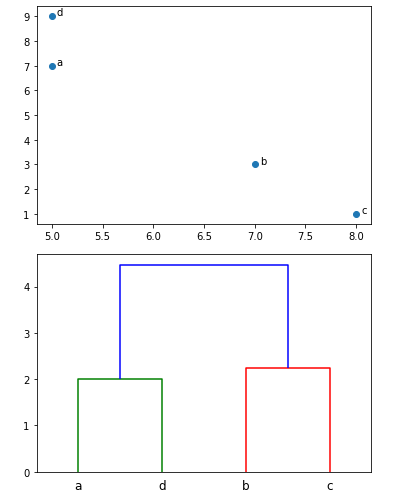
\includegraphics[width=.6\linewidth]{figs/deno/toy-dendrogram.png}
  \caption{Top: A simple scatter plot of some arbitrary data points 
  \newline Bottom: A dendrogram illustrating the agglomerative process. 
  \newline Notice that $(b,c)$ are merged after $(a,d)$ indicating that latter are more similar}
  \label{fig:toy-dendrogram}
\end{figure}

 
Under hierarchical clustering, any number of final clusters can be set. 
This means that the number of final clusters is determined up to human discretion, thereby not guaranteeing clearly defined clusters.

 
\subsection{Evaluating Clusters}
 After the clusters have been generated, it is useful to evaluate the result.
%  well the observations have been grouped. 
One way to do this is with the Davis-Bouldin index (DB-index or DB-criterion) is defined as the ratio of the “within-cluster”-distance and “between-cluster”-distance. “Within-cluster”-distance is a description of dispersed elements of a cluster is and “between-cluster”-distance  is a description of how far apart the cluster are from each other. This means that a low DB-index is an indication of a good clustering result. 

In the context of this, the information gained from the DB-index is minimal.
This is because it as well as all other numerical evaluations,  depend on a ground truth of how to correctly quantify the similarity distance. 
The index may provide some insight, however, we expect the true information gain to be minimal and its ranking to be biased.


As a closing remark, we acknowledge that there is no general standard for what constitutes a “reasonable clustering” on account of it being highly domain-dependent.
Human inspection remains a vital tool for evaluating final clusterings\cite{79-SilhouetteAnalysis}. 
In order to discuss the clustering results from a visual perspective, we define the terms \textit{Fuzzy} and \textit{Crisp} as seen in \Cref{def:cluster_defs_fuzz,def:cluster_defs_cri}.

\begin{definition}\label{def:cluster_defs_fuzz}
A cluster is \textbf{fuzzy} if its members appear spread out and with seemly little relation to each other.  
For a "good" clustering result, we wish to minimize the number of fuzzy clusters. 

\end{definition}

\begin{definition}\label{def:cluster_defs_cri}
A cluster is \textbf{crisp} if its members create a clear silhouette with seemly a clear correspondence.
For a "good" clustering result, we wish to have as many crisp clusters as possible 
\end{definition}

\chapter{Similarity Distance Algorithms}
\label{ch:3}

In this chapter, we present seven different similarity distance measures. 
First, we describe four that are parameter-free, then we describe three algorithms that require a parameter. 
By chance, all of the parametric methods are based on Edit Distance, so we briefly explain how its construction as well. 


The methods have largely been chosen due to their prominence in the existing literature\cite{58-UCRTime,70-SimilarityDistances,8-EffectivenessStudy,53-TimeSeries,52-OnlineEfficient}. 
However, we present two newer algorithms, one parameter-free and one that requires a parameter.
They are presented at the end of their respective groupings. 
 
As was the case in the previous chapter, large portions here are based on the report created for \textit{TDT4501 Computer Science, Specialization Project}


\section{Parameter-Free Measures}
% The advantage of these parameter free methods is, as their names tell us, that they do not have parameters and they are “out of the box” ready. 

\subsection{Euclidean Distance (Ed)}
As noted in \Cref{ch:2}, the Euclidean distance (Ed) is a way to quantify the distance between two points in space. 
There is a naive extension of that principle that lays the foundation for a Euclidean Distance measure for trajectories\cite{44-FastSubsequence, 8-EffectivenessStudy, 24-ReviewTrajectory,86-ComputingMinimum}. This method would be to compute the mean point-point distances in a lock-step manner as seen in \Cref{eq:ed}.

\begin{equation}\label{eq:ed}
Ed(A, B) = \frac{1}{n}\cdot \sum_{i=1}^{n}d(a_i, b_i)
\end{equation}
where the distance between corresponding points is the $L_2$-norm as defined in \Cref{eq:l2norm}

Its simplicity comes with a couple of disadvantages, one notable one is that it requires the trajectories to be of equal length. 
In the cases where the number of points does not match one would have to adapt the data, potentially altering the original observations. 
Furthermore, computing distance in a lock-step manner means that it is sensitive to local time shifts and noise\cite{12-RobustFast}. 

Even with these limitations, this measure is included for its simplicity.  Previous work has shown that it holds remarkably well up to more advanced methods\cite{26-QueryingMining}, further encouraging us to examine this metric. 


\subsection{Dynamic Time Warping (DTW)}

As stated in \Cref{sec:elasticity} an elastic measure is needed in order to handle local time shifts and Dynamic Time Warping (DTW) is precisely that. 
DTW was originally designed for speech recognition which means that it handles relative lag seamlessly\cite{45-CrosswordsReference, 27-DynamicTime}.
This makes it a prevalent choice for examining similarity under temporal drift.
The idea behind this algorithm is to stretch and contract time such that a favorable alignment of the input trajectories can be found. 


\Cref{fig:dtw_cost_path} illustrates the implementation of DTW. 
The computation begins by taking input trajectories $A$ and $B$ and constructing a full cost matrix $C$. This matrix keeps all pairwise distances  between the trajectories' elements. 
We use the $L_2$ norm for point-to-point distance computation as is common for DTW\cite{5-ComputingVisualizing}. 
After the matrix has been constructed, the next step is to iteratively search through  $C$ and find the optimal warping path, $p$. 
The optimal warping path is the set of point-point pairings, entries of $C$, that  minimizes the accumulated cost. 
The accumulated cost along the warping path is the DTW distance between the trajectories. 
\Cref{fig:ed_dtw_diff} exemplifies how the Euclidean distance and DTW differ with respect to time-shift. 

% how this approach stands out from 
% for an illustration of how the points are aliened under a lock-step measure like the Euclidean Distance and DTW.

\begin{figure}[h]
\centering
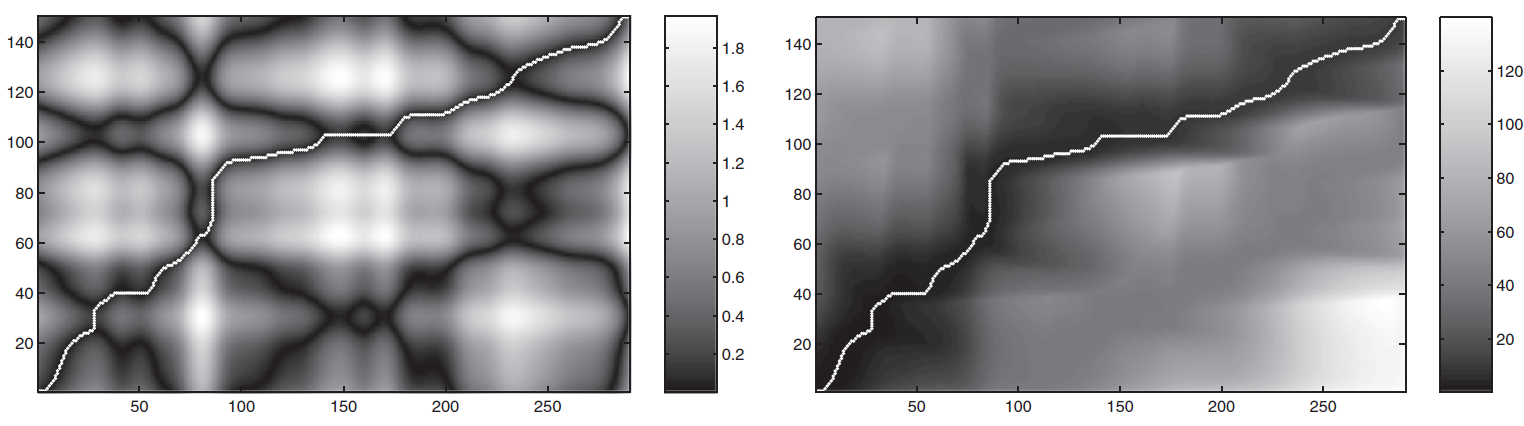
\includegraphics[width=.7\textwidth]{figs/algos/dtw_C_p.png}
\caption{Cost matrix $C$ (left) and accumulated cost matrix $C'$ which the optimal warping path $p$ (right) . Figure copied from \cite{27-DynamicTime}}
\label{fig:dtw_cost_path}
\end{figure}

\begin{figure}
\centering
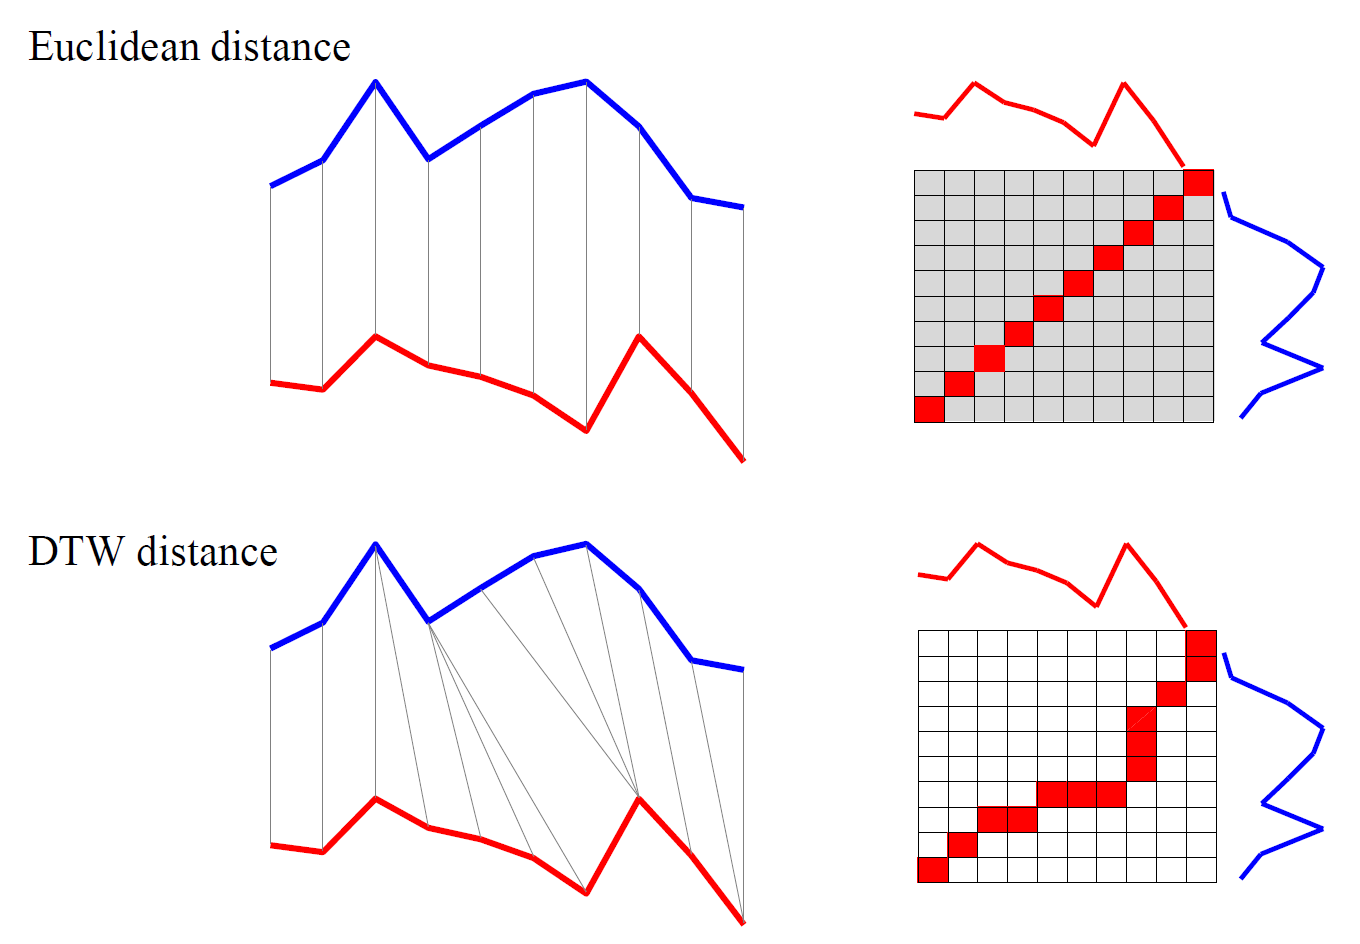
\includegraphics[width=.7\textwidth]{figs/algos/ed_dtw_diff.png}
\caption{An illustration of how the Euclidean forces a lock-step computation whereas DTW realigns the trajectories. Figure copied from \cite{58-UCRTime}}
\label{fig:ed_dtw_diff}
\end{figure}


The main drawback of DTW is that it weights all points of both trajectories equally and thus it is not robust to noise. 
A naive implementation of DTW would forcefully align the start- and endpoints of the two trajectories which can disproportionately punish trajectories that are overall similar\cite{4-ElasticPartial}. 
Generating the cost matrix quickly becomes expensive due to pairwise comparing all points of the input trajectories which makes it less suited for large data sets \cite{27-DynamicTime}. 

Its shortcomings have inspired iterations of DTW that seek to address them. Some remark that constructing a full cost matrix may not be needed, and some seek to speed up how to iterate through $C$\cite{5-ComputingVisualizing}. We note that a popular choice is \textbf{FastDTW}, which is a parameterized version of DTW. 
As the name indicates, it is much faster than the naive implementation yet gives comparably accurate results\cite{9-FastDTWAccurate}. 
Nevertheless, this thesis shall only focus on the parameter-free version.



\subsection{Hausdorff Distance (Hd)}
% This distance measure is a metric that weights shape similarity, meaning the temporal aspect or order of trajectory elements does not matter 
This technique is often discussed in relation to polygons and sets\cite{49-HausdorffDistance} however it is applicable for time-series data as well. 
A consequence of its geometric origin is that the trajectory direction no longer affects the final result, the notion of a first or last trajectory element is not kept\cite{86-ComputingMinimum}. 
The Hausdorff distance from  $A$ to $B$ is the maximum of the minimum of all pairwise distances, see \Cref{eq:Hd-directed}\cite{48-ComputationalGeometrya} 

\begin{equation}
\label{eq:Hd-directed}
\widetilde{Hd}(A, B) = max_{a\in A}\big\{ \, min_{b\in B } \enspace d(a, b)\,\big\}
\end{equation}

where $d(a, b)$ is any metric distance function, here the $L_2$-norm is used. 
The distance function described in \Cref{eq:Hd-directed} is not symmetric and thereby not a metric\cite{14-EfficientAlgorithm}. The function is referred to as the directed Hausdorff distance. 
To make the Hausdorff metric, it is defined as the maximum  of the two directed results. 
This makes the function symmetric, so that it fulfills the requirements for a metric, see \Cref{eq:Hd-metric}.

\begin{equation}
\label{eq:Hd-metric}
Hd(A, B) = max\big\{ \,\widetilde{Hd}(A, B), \;\widetilde{Hd}(B, A)\big\}
\end{equation}

Since we can compare any point in A to any point in B this measure is elastic. 
All points of the trajectories are weighted equally which makes it is sensitive to noisy data. 
Additionally, the effect of reducing the similarity score to the distance between two points from each trajectory is that information about the trajectories' overall shape is lost. 
The metric is highly sensitive to noise\cite{51-HausdorffDistance}. 
Lastly, we need to work out both of the directed distances to get the similarly score. This means more work per trajectory pair than naturally symmetric measures such as Ed and DTW.  


\subsection{Symmetrized Segment-Path Distance (SSPD)}
As the  Hausdorff distance, Symmetrized Segment-Path Distance (SSPD) method is a spatial only algorithm that largely disregards the direction of the trajectories.
It is was developed from the same principles as the Hausdorff distance, but with the addition of being able to account for  the trajectories as a whole.\cite{43-TrajectoryDistance, 50-ReviewPerspective}. 
The algorithms explained so far have used the trajectory elements directly as the basis for the computations. For SSPD, this is no longer the case, and thus we define notation and terms to describe this algorithm.  

 In line with  \Cref{tb:notation}  $a, b$ are elements of Trajectories $A, B$ respectively . 
 A \textit{segment} is the line between two consecutive points, and we use $\breve{a}$ to denote a segment of $A$. Using indexes,  $\breve{a}_i$ is the line between $a_i$ and $a_{i+1}$. 

Next we define the \textit{point-to-segment distance} as shown in \Cref{eq:sspd-ps}. This distance function requires us to find the point’s orthogonal projection onto the segment. 
If it is within the segment, the distance will be the  $L_2$-norm between the original point $a$ and its projection $\dot{a}$.
Otherwise, the  $L_2$- norm to segment's end points is computed nearest those distances becomes the point-to-segment distance.  

\begin{equation}
\label{eq:sspd-ps}
d_{ps}(a_i, \breve{b}_j) =  \begin{cases}
d(a, \dot{a})  &\text{if} \enspace \dot{a} \in \breve{b}_j\\
min\{ d(a_i, b_j), d(a_i, b_{j+1})\}  &\text{otherwise}
\end{cases}
\end{equation}
Where $\dot{a}$ is the orthogonal projection of point  $a$ onto segment  $\breve{b_j} $ and $d$ is the $L_2$-norm. 

From point-to-segment distance, \textit{point-to-trajectory distance} is defined as shown in \Cref{eq:sspd-pt}. 
The point-to-segment distance is computed for all the segments of the trajectory and the lowest one becomes the point-to-trajectory distance.

\begin{equation}
\label{eq:sspd-pt}
D_{pT}(a_i, B) = min_{\breve{b} \in B} \big\{ \, d_{ps}(a_i, \breve{b})\, \big\}
\end{equation}
The \textit{Segment-Path-Distance} (SPD) is directed.
It is defined to be the mean of the all point-to-trajectory distances from points of the first trajectory to the second trajectory, \Cref{eq:sspd-spd}.

\begin{equation}
\label{eq:sspd-spd}
SPD(A, B) = \frac{1}{n_A} \sum_{i=1}^{n_A} D_{pT} (a_i, B)
\end{equation}
As with the Hd, this distance measure is made symmetric by computing both directed versions first. However unlike Hd, the final result is the mean of the directed results. The name comes from this last step and the final formula is shown in \Cref{eq:sspd-main}.
 
 \begin{equation}
\label{eq:sspd-main}
SSPD(A, B) = \frac{\big( \, SPD(A, B) + SPD(B, A)\, \big)}{2}
\end{equation}

 
The creators of SSPD note that if one were to use the max function rather than computing the mean upon symmetrification this algorithm would be identical to the Hausdorff function\cite{50-ReviewPerspective}. 
They note that with their method, this distance function becomes more robust to noise when calculating the mean, as opposed to maximizing or minimizing.  
Moreover, they commend SSPD for being parameter-free as well as not relying on interpolation between two observed point, preferring to strengthen the importance of observed data. 
As a closing remark, we note that SSPD does not fulfill the requirements of a metric. 

\section{Parameterized Measures}


 In this section, we have described measures that require a parameter. 
 All of them are based on String Edit Distance (SED) which is a similarity measure designed for strings.  
 The idea is to count the number of \textit{edits} needed to convert one string into the other using the edit operations are insert, delete and replace.  
 Due to the strings' natural discretization, it is trivial to determine whether or not two symbols are matching. 
There are variations of implementation but a common choice is to let the cost of an \textit{edit} be 1, creating a formula as seen in \Cref{eq:ed_string}:  

\begin{equation}\label{eq:ed_string}
    \text{SED}(S1, S2) = \begin{dcases}
        \quad |S1| & \text{if }  |S2| = 0\\
     	\quad |S2| & \text{if }  |S1| = 0\\
        \quad \text{SED}(S1,\; S2) & \text{if }  |S1| =|S2| \\
        \begin{aligned}
        1 + min\big\{   & \text{SED}(Rest(S1), \; Rest(S2)) \\
              	     & \text{SED}(Rest(S1), \; S2) \\
           		    & \text{SED}(S1, \; Rest(S2)) \\
        \end{aligned} & \text{otherwise}
  \end{dcases}
\end{equation}

Real data does not let itself be discretized as fortuitously as strings, thereby leading to the creation of the algorithms below. 
The measures differ in how they have adapted SED for time series data, and the role of the parameter value changes as well. 
 

% \subsection*{FastDTW}
% As its name indicates, this algorithm is a modification of DTW. We remarked that DTW is expensive in both time and space complexity. FastDTW archives linear complexity on both fronts, but does introduce a parameter to do so \cite{9}. 

% The idea behind this is to first run the algorithm at coarse resolution, compute a projected warp-path and then rerun the algorithm at a finer resolution to tune the path. This is repeated until we have reached the original resolution. Two of the most important ways this algorithm is sped up are the following. 
% Firstly, fewer cells of the cost matrix need to be calculated or evaluated. Secondly, data abstraction means that the cost of DTW itself is greatly reduced. This means a great improvement in cost, however at the expense of no longer being parameter free. The parameter in question is a radius parameter which determines how much the projected optimal path can deviate from the one found at the previous iteration. See FIGURE for an illustration of how the iterative search plays out with the radius parameter. WILL NOT INCLUDE


% One way we could speed up DTW is by introducing a \textit{radius parameter}, and this algorithm is called FastDTW\cite{9}. This approach first runs the algorithm at a coarser resolution, and then reruns itself in order to tune the result. This means a great improvement in cost, however at the expense of no longer being parameter free. Nevertheless we have chosen to include both DTW and FastDTW as part of our survey to examine the impact of this alteration. 

\subsection{Edit Distance on Real Sequence (EDR)}

Edit Distance on Real Sequence (EDR)\cite{12-RobustFast} introduces a threshold parameter $\epsilon$ that determines if two trajectory elements are “matching”. 
Crucially, there can be no partial matches so the point-to-point distance is either 1 or a 0 as shown in \Cref{eq:edr_subcost}.

\begin{equation}\label{eq:edr_subcost}
d_{edr} (a, b) = \begin{cases}
0 \quad &\text{if } \quad | a_{LNG} -b_{LNG}|\leqslant  \epsilon  \text{ and } | a_{LAT} -b_{LAT}|\leqslant  \epsilon    \\
1 \quad &\text{otherwise}\\
\end{cases}
\end{equation}
where $\epsilon$ is the threshold parameter. After determining whether or not two points match with the subcost function we get the full EDR is shown  algorithm as seen in \Cref{eq:edr_main}


\begin{equation}\label{eq:edr_main}
    EDR(A, B) = \begin{cases}
        n_A \qquad &\text{if } n_B = 0\\
        n_B \qquad &\text{if } n_A = 0\\
        \begin{aligned}
        min\big\{ & EDR(\text{ Rest}(A), \text{ Rest}(B)) + d_{edr}(a, b),\\
              & EDR(\text{ Rest}(A), B) + 1,\\
              & EDR(A, \text{ Rest}(B)) + 1 \big\}
        \end{aligned} & \text{otherwise}
  \end{cases}
\end{equation}where $a, b$ are the leading elements of $A, B$.  

The main advantages of EDR are its resistance to noise and the ability to handle local time shifts. 
It is resistant to noise because of how it maps the distance between elements to a binary 1 or 0. 
Toohey and Duckham asserted that EDR performed well in spite of variance in the sampling rate\cite{17-TrajectorySimilarity}.

EDR is not a metric measure as it does not fulfill triangle inequality, but it meets other requirements of metrics. 
Furthermore, it evaluates similarity as trajectory elements, not taking into account the trajectories' overall shape. 
We have chosen to include this algorithm as it is a well-studied algorithm. 
Its prevalence in the literature has led it to be studied alongside DTW and Euclidean Distance. 


\subsection{Edit Distance with Real Penalty (ERP) }
Edit Distance with Real Penalty (ERP) was designed to bridge the gap between metrics distance functions and local time shifting tolerant ones. \cite{13-MarriageLpnorms}. The design of EDR began with the $L_1$-norm \Cref{eq:manhatten}

\begin{equation}\label{eq:manhatten}
Dist_{L1} (A, B) = \sum_{i=1}^{n} d(a_i, b_i) \qquad \text{where} \qquad d_{L_1}(a_i, b_i) = \sum_{j=1}^{p}|a_{i,j}- b_{i,j}|
\end{equation}

From SED, the notion of a \textit{gap element} is introduced. 
A gap element is a symbol that could have been deleted from string $S1$ but instead is inserted into string $S2$.
The point-to-point distance function would then become what is shown in \Cref{eq:erp_ed}. 

\begin{equation}\label{eq:erp_ed}
    d_{ed}(a_i, b_i) = \begin{cases}
        0 &\qquad \text{if } a_i = b_i \\
        1 &\qquad \text{if } a_i \text{ or } b_i \text{ is a gap } \\
        1 &\qquad \text{otherwise } \\
    \end{cases}
\end{equation}

% SED, just as the $L_p$ norms, is a metric distance measure, but to further develop this algorithm it needs to accommodate real values.
Rather than using a constant value to penalize all edit operations uniformly like EDR, ERP differentiates between gap elements and non-gap elements. 
This distinction is important so that it will be tolerant to local time sifting. 
Gap elements are penalized with a constant value, while non-gap elements have a real-value cost based on their value. 
The parameter of ERP,  $g$, is the reference value for cost computation, and the point-to-point distance function is seen in \Cref{eq:erp_sub}

\begin{equation}\label{eq:erp_sub}
     d_{epr}(a_i, b_i) = \begin{cases}
        |a_i-b_i| & \qquad \text{if  neither is a gap} \\
        |a_i-g|   & \qquad \text{if } b_i \text{ is a gap} \\
        |b_i-g|   & \qquad \text{if } a_i \text{ is a gap} \\
     \end{cases}
 \end{equation}
 
 Again, the trajectory distance function is an adaption of SED, and the full algorithm for ERP is shown in \Cref{eq:erp_main}
%  but was no longer a metric after it.
\begin{equation}\label{eq:erp_main}
    ERP(A, B) = \begin{dcases}
        \quad \sum_{i=1}^{n_A}|a_i - g| & \text{if }  n_B = 0\\
        \quad \sum_{i=1}^{n_B}|b_i - g| & \text{if }  n_A = 0\\
        \begin{aligned}
        min\big\{   & {ERP}(Rest(A), \; Rest(B)) + d_{erp}(a_1,\;  b_1),\\
              	    & {ERP}(Rest(A), \; B) + d_{erp}(a_1, \; g),\\
           		    & {ERP}(A, \; Rest(B)) + d_{erp}( b_1,\; g) \big\}
        \end{aligned} & \text{otherwise}
  \end{dcases}
\end{equation}

The main drawback of this method stems from the characteristic that makes it a metric, using differences of real values as costs.
This method is a metric as long as $g$ is constant, making the cost of an edit vary the location of the trajectory element. 
However, this makes ERP sensitive to noise\cite{12-RobustFast}. 


\clearpage
\subsection{Move-Split-Merge (MSM)}
Move-Split-Merge (MSM) \cite{40-MoveSplitMergeMetric} is similar to the aforementioned to the other SED-based approaches in that it calculated the similarity score from how many operations are needed to transform one trajectory into another one.
This algorithm is tolerant to temporal misalignments and translation invariant\cite{53-TimeSeries} as are EDR and ERP.  
What distinguishes this algorithm from them is how insertions and deletions are handled.
The MSM cost model uses both the value of the element being modified as well the adjacent one whereas ERP only uses the element being modified and EDR uses a constant cost for all operations. 


As the name of this algorithm indicates, the possible operations are Move, Split, and Merge, which are then used to emulate the established Edit Distance operations Insert, Delete, and Substitute.
The Move operation is a renaming of does the same as Substitute.
The Split operation inserts a copy of a given value directly after itself, and the Merge operation deletes a value if it is immediately followed by a matching value\cite{53-TimeSeries}. In other words, Split and Merge are each others’ inverse.
The Insert operation becomes a Split followed by a Move, while Delete becomes a Move followed by a Merge. 
The MSM parameter, $c$, is  a non-negative value that determines the cost of every Split and Merge operation. See \Crefrange{eq:msm-start}{eq:msm-end} for details. 

\begin{align}
 A  &= [a_1, \cdots , a_{i-1},\, a_i,\, a_{i+1}, \cdots  , a_{n_A}] \nonumber \\
 \nonumber\\
\text{Move}_{a_i \rightarrow b_j}(A)  &= [a_1, \cdots , a_{i-1},\, b_j,\, a_{i+1}, \cdots  , a_{n_A}] \label{eq:msm-start} \\
\text{Cost} \big\{ \text{Move}_{a_i \rightarrow b_j}(A) \big\} &= d(a_i, b_j) \\
\nonumber \\
\text{Split}_{a_i}(A) &= [a_1, \cdots , a_{i-1},\,a_i,\, a_i,\, a_{i+1}, \cdots  , a_{n_A}]\\
\text{Cost} \big\{ \text{Split}_{a_i}(A) \big\} &= c \\
\nonumber \\
\text{Merge}_{a_i}(A) &= [a_1, \cdots , a_{i-1},\, a_{i+1}, \cdots , a_{n_A}] \\
\text{Cost} \big\{ \text{Merge}_{a_i}(A) \big\} &= c \label{eq:msm-end}
\end{align}

Recall that the $\text{Merge}_{a_i}(A)$ operation is only permitted if $a_i = a_{i+1} $. 
This algorithm fulfills the requirements of a metric and thus it can be used for indexing and clustering techniques that are designed to function in metric spaces. 
In terms of computational cost and accuracy, we refer to work done by Bagnall et. al. which alludes to MSM being comparably efficient to ERP and more tolerant to noise DTW\cite{56-GreatTime}.

 

 
 \clearpage
\section{Summary of Algorithms}

\Cref{tab:meas_comp} summarizes some trajectory similarity features. 
Remark that none of the measures have matching rows, further indicating that the meaning of trajectory similarly varies with technique implementation. 


We reiterate that large portions of this chapter stem from the report that was mentioned at the beginning. 
Still, there is not a complete overlap of the measures discussed in that report and this thesis. 



% Euclidean distance is the only measure that does not account for local time shifts, and    
% From all aspects apart from "overall shape" similarity, there has been about half and half if they measures fulfilled the requirements.

% distance functions satisfy the requirements of metricity 

% https://www.tablesgenerator.com/latex_tables

\begin{table}[t]
\centering
\caption{Quick view of some aspects the similarity distance measures}
\label{tab:meas_comp}
\resizebox{\textwidth}{!}{%
\renewcommand{\arraystretch}{1.5}
\begin{tabular}[h]{*{6}{|p{1.8cm}}|}
 \hline
\textbf{Name}   & \textbf{Metric } & \textbf{Single \newline Element } & \textbf{Time Shifts} & \textbf{Parameter} & \textbf{Noise \newline Tolerant}      \\ 
\hline
\textbf{ED} 		 & Yes    & Yes     & No  & No    & No      \\ 
\hline
\textbf{DTW}      & No:    &Yes    &Yes    & No   & No    \\ 
\hline
\textbf{Hd}       & Yes    & Yes        &Yes     & No     & No      \\
\hline
\textbf{SSPD}      & No    & No          &Yes   & No   & Yes  \\ 
\hline
\textbf{EDR}       & No   & Yes    & Yes       & Yes     & Yes   \\
\hline
\textbf{ERP}       & Yes   & Yes    & Yes      & Yes    & No    \\
\hline
\textbf{MSM}      & Yes   & No    & Yes   & Yes   & Yes \\ 
\hline
\end{tabular}
}
\end{table}


% double check the noise tolerances, use checkmarks?

\chapter{Existing Surveys of Time-Series  Similarly Distance }
\label{ch:4}

With there being a large number of time-series similarity distance functions, it follows that there is an accompanying body of work which seeks to consolidate the scattered information.
In this chapter we go over some of the those studies, and provide further motivation for the work conduced in this thesis. 

We identify two varieties of studies: those that rank the measures according to some predetermined standard and those that provide comprehensive feature descriptions. 

% and label them as surveys that analyze the measures on their own merits (grounds? features?) and those that run experiments to compare and contrast various ones.

%%%%%%%

%There is an existing body of work that seeks to consolidate the scattered information on different time series. [59, 58, 56,27, 24,17, 8]. The principal methods we noticed being brought forth across different reviews were DTW, and Euclidean distance, as well the Edit Distance based algorithms ERP and EDR. We acknowledge that there is a fifth measure, Longest Common Subsequence  (LCSS), which is comparably well-known and analyzed. Nevertheless we decided to exclude LCSS from this thesis to limit scope. With Euclidean distance and DTW being near (omnipresent) , comparing them to other measures gives familiar context for previously non-examined methods. 

% We identify two “primary veins'' previous endeavors have been taken in order to compare the trajectory similarity measures; Either reviews that specify features of the measures abstractly [24] or performing data mining tasks in order to achieve numerical results[59]. Most frequently it was a bit of both, with most effort and weight being placed on the mining tasks. 


%We identify two primary categories that previous endeavors have taken in order to compare the trajectory similarity measures.The first one are reviews that specify features and theoretical computational characteristics of the measures [24, 48]. The other kind are those that opt to implement the measures and run tests that produce numerical results[59, 56, 8]. Naturally, this approach included a brief discussion of the measures'  implementation details. 

\section{Ranking Studies }

\subsection{Trajectory Clustering}
P. Besse et.al, the creators of SSPD, prefaced their work by examining existing distance functions for trajectories\cite{50-ReviewPerspective}. 
The measures were categorized into "shape-based" ones and “warping-based” ones, referring to how a measure accounted for the temporal component of the trajectories. 

Their work studied the different clusterings that were obtained through clustering tasks where the distance function varies.
They determined that the “shape-based" distance measures gave better results than the “warping-based" ones. 
However, they concluded this based on the cluster quality criteria they defined.
The criterions resembled the Davies-Bouldin Index, but it was deconstructed so that the “between-like” and “within-like” evaluations were presented individually. 

% \clearpage

\subsection{Time Series Mining}
H. Din et.al did an experimental comparison of both time-series representations and similarity distance measures in an effort to categorize mining techniques \cite{26-QueryingMining}. 
Their motivation was that other studies had been too narrowly focused on a specific measure, or that the conclusions were too optimistic. 

Their experiments used a nearest neighbor classifier to evaluate nine different similarity measures and eight different data representations.
The thoroughness of their setup was further emphasized as they ran their experiments on 38 different time-series data sets. 
While data sets originated from a variety of real sources, they were all suited to the mining task classification. 



Under classification, labels are given to each time-series based on their similarity are to other series. Typically the observations receive one label each. 
One key way classification differs from clustering is that in that classification results rend to be simpler to evaluate. 
They are distinct usages of similarity distance and the conclusion drawn in this work are oriented towards the classification results. The features of the similarity measures themselves were not emphasized.  



\section{Non-Ranking Studies}

\subsection{Review of Trajectory Measues}
Work done by N. Magdy et.al examined 13  different trajectory similarity measures\cite{24-ReviewTrajectory} in a theoretical manner.  
Of the seven discussed in \Cref{ch:3}, five of them were examined by the authors.

Their work did not include an experimental component. 
The measures were categorized based on implicit similarity definition, and the traits of each measure.
Namely if whether or not they were noise-tolerant, could handle locally time-shifted data, if they fulfilled the requirements of metricity and their computational cost.

Furthermore, the researchers contrasted how the required data format varied, and how that affected the notion of similarity.
The work concluded by underlining that there is no measure that is the most appropriate for any given data set. 
They expressed a wish for a generic trajectory similarity measure which could then be adapted to accommodate the desired specific type of similarity depending on the application. 

\subsection{Effectiveness Study}
H. Wang et.al conducted an effectiveness study on six trajectory similarity measures\cite{8-EffectivenessStudy} and half of them that were also discussed in \Cref{ch:3}. 
After a theoretical summary of the measures, they set up an experiment to test their \textit{effectiveness}.
The study was realized on a data set where the researchers had intentionally altered some of the entries. This was done so that the advantages and drawbacks of their selected measures would be highlighted.


One of the aims of this study was to lay the foundation for a new benchmark that could objectively quantify the effectiveness of similarity measures. 
They tested the measures under the following trajectory transformations: a simulated sampling rate change, added noise, and shifts of the trajectory, both temporal and spatial. 
The benchmark compared the original trajectory to a transformed one, changing which similarity measures were used. 
The measures that recognized them as the same trajectory, or as similar trajectories, were classified as “passing" under that transformation. 
Using the experimental results they created a table that summarized each measures' effectiveness under the various transformations.



\subsection{Vehicle Trajectory Survey}
Abas et.al did a comprehensive survey of trajectory data\cite{85-VehicleTrajectory} wherein they focused on vehicular data. 
Their work investigated how the inherent inaccuracies of GPS data affect the quality of trajectory analysis.
They surveyed different trajectory representations, noting the advantages and disadvantages of each. 
Next, they discussed processing techniques that are used to handle the drawbacks of a given representation. 
Some of the trajectory representations they brought up were road-network constrained trajectories, binary-encoded trajectories, and hash-based trajectories. 


A selection of similarity measures was specified for each type of representation and they noted whether or not a measure fulfilled certain properties. 
The properties in question were metricity, parameter dependency, ability to handle local time shifts, and ability to handle noise. 
Four of the measures that were were brought up in their work are also discussed in this thesis. One of the research gaps they remarked was how one would process  "big trajectory data".
 
 
\section{Our Contribution}

This thesis seeks to add the body of work that compares and contrasts trajectory similarity distance measures.
The experiment we conducted here is based on various elements of the aforementioned studies. 

We did not see a selection of measures matching ours; notably, few studies examine MSM and SSPD which is in all likelihood a testament to their novelty. 
We remark that the efforts described in  “Trajectory Clustering” and “Vehicle Trajectories” have had major influences on our work. 
We hope to provide a comprehensive comparison wherein feature description and clustering results play equally important roles.


\chapter{Set Up and Method}
\label{ch:5}

\section{Technical Environment}

The experiments carried out in this thesis were executed in Google Colaboratory (Colab) which is a Google-hosted implementation of Jupyter Notebook\cite{72-GoogleColaboratory,73-ProjectJupyter}. 
The base components of a Notebook are cells that can be grouped thematically. 
The cells can contain code or markdown, smoothing out the transition between coding and writing which is conducive to a smooth workflow.
Another key advantage of this setup is the ability to work from anywhere. This is possible as the notebook is being executed by Google's cloud servers; there were no specific hardware dependencies for the computations. 

Given the choice to work in the Jupyter environment, Python becomes the natural choice of programming language\cite{74-WelcomePython}. 
This choice is further substantiated by the prevalence of existing modules made for data analysis.
There are significant computational gains from using an extension of Python called Cython\cite{75-CythonBest}. 

We used the module \mintinline{Python}{trajectory_distance}\cite{43-TrajectoryDistance} to compute almost all the distance functions. 
There were no implementations of Euclidean Distance and Move-Split-Merge, so we coded our own. 
The former was trivial to implement.
As for the latter, the creators of MSM had published a JAVA implementation of their algorithm. 
Using that code as a guide we created a “Pure-Python”-Cython cell in the Jupyter Notebook which was used for its similarity distance computation.  
Due to the differences in implementation, we cannot evaluate the algorithms’ time complexity fairly.


\clearpage
\section{Data Set}
In this thesis, the aim is to gain information about various similarity measures and consequently, the setup should be as data set agnostic as possible.
With this in mind, we first generated synthetic data for initial test runs and then modified real trajectory data which we could use for more extensive tests.

% This is in part because there could be some underlying similarities that are. It is hard to with synthetic data, and the advantage of using real data is that we may gain insight from it.  As far as deciding on which data set we will use, the decision has not been made yet. Currently there are two data sets that seem interesting enough to examine more closely.  




\subsection{Synthetic Trajectory Generation}

% The motivation behind using a synthetic data set first is so that it is possible to have control over the input data while getting started. Primarily we wish to ensure that the size of the data set is not too large as both clustering and the similarly measures could take a lot of computing time. Ideally we would have just a handful of trajectories for the first clustering jobs, as well as limiting the length of the initial trajectories. Real data sets could have many hundreds of trajectories and/or hundreds of values per trajectory and are therefore not well suited for early testing.


The generation of synthetic data was the first step of this experiment. 
The aim of doing this  was so that we could determine the architecture of the experiment validate that the distance functions were producing reasonable results.  
% When generating the trajectories, the data format was intentionally identical to that of the real data set. 
The generated data set can be seen in \Cref{fig:synthetic-data}. 
It quickly became evident that the data was too random to serve as a basis for the similarity algorithms.
Rather than using more advanced methods for creating synthetic data such that it could potentially accurately represent a complex system, we chose to examine trajectory real data.
 


\begin{figure}
\centering
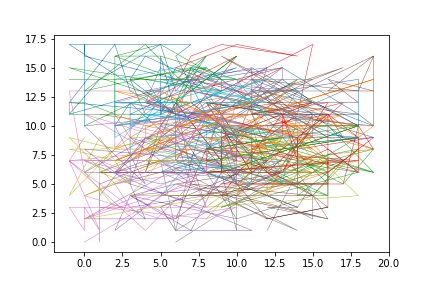
\includegraphics[width=.7\textwidth]{figs/traj/SYNTHETIC.png}
\caption{Synthetic data set of randomly generated trajectories.}
\label{fig:synthetic-data}
\end{figure}



\subsection{Real Trajectory Preprocessing}

The data set that was selected for this thesis is a taxi trajectory data set with  over 1.7 million rows\cite{3-TaxiTrajectory}. 
In addition to a large number of rows, there were superfluous columns such as what type of taxi ride it was and whether or not the trip was on a weekend. 
The first step of the data preprocessing was to remove these attributes from the rows.  
Next, a random subset consisting of just over 500 trajectories was selected. 
They were given unique IDs their routes can be seen in \Cref{sfig:real-med}. 


\clearpage
As mentioned in the \Cref{ch:3}, the Euclidean distance may only evaluate trajectories of the same length. 
Rather than interpolate to add data points– or compute the information gain of the trajectory elements and then get rid of the least informative ones, we truncated all trajectories to the same length. 
Moreover, initial tests indicated that a set of 500 trajectories was still too voluminous and time consuming to analyze. '
As a result, we created two subsets of those 500 raw trajectories, one significantly smaller than the other so that tests could be run quickly. The truncated trajectory sets are depicted in \Cref{sfig:real-trunc,sfig:real-trunc-mini}


% em dash  –

As seen in \Cref{fig:real-datasets} the trajectories are fairly spread out, and so we normalized the range of the coordinates of the data set.
We scaled the data so that they would be in the same value range and we could examine similarity on a seemly arbitrary set of lines. '
Without this step, trajectories spanning a small identical geographical area would artificially receive a higher similarity score by being near each other, regardless of shape similarity.
This is the re-scaling disconnected data from their real world source while maintaining a general similarity shape from trajectories that followed the same roads. 
Finally, we remark that the re-scaling was done with simplification of independently scaling the latitudinal and longitudinal dimensions, further distorting their relation to the underlying road network. 
The final scaled data set is graphed in \Cref{fig:scl-datasets}.


\begin{figure}[h!]
\centering
\begin{subfigure}{.451\textwidth}
    \centering
    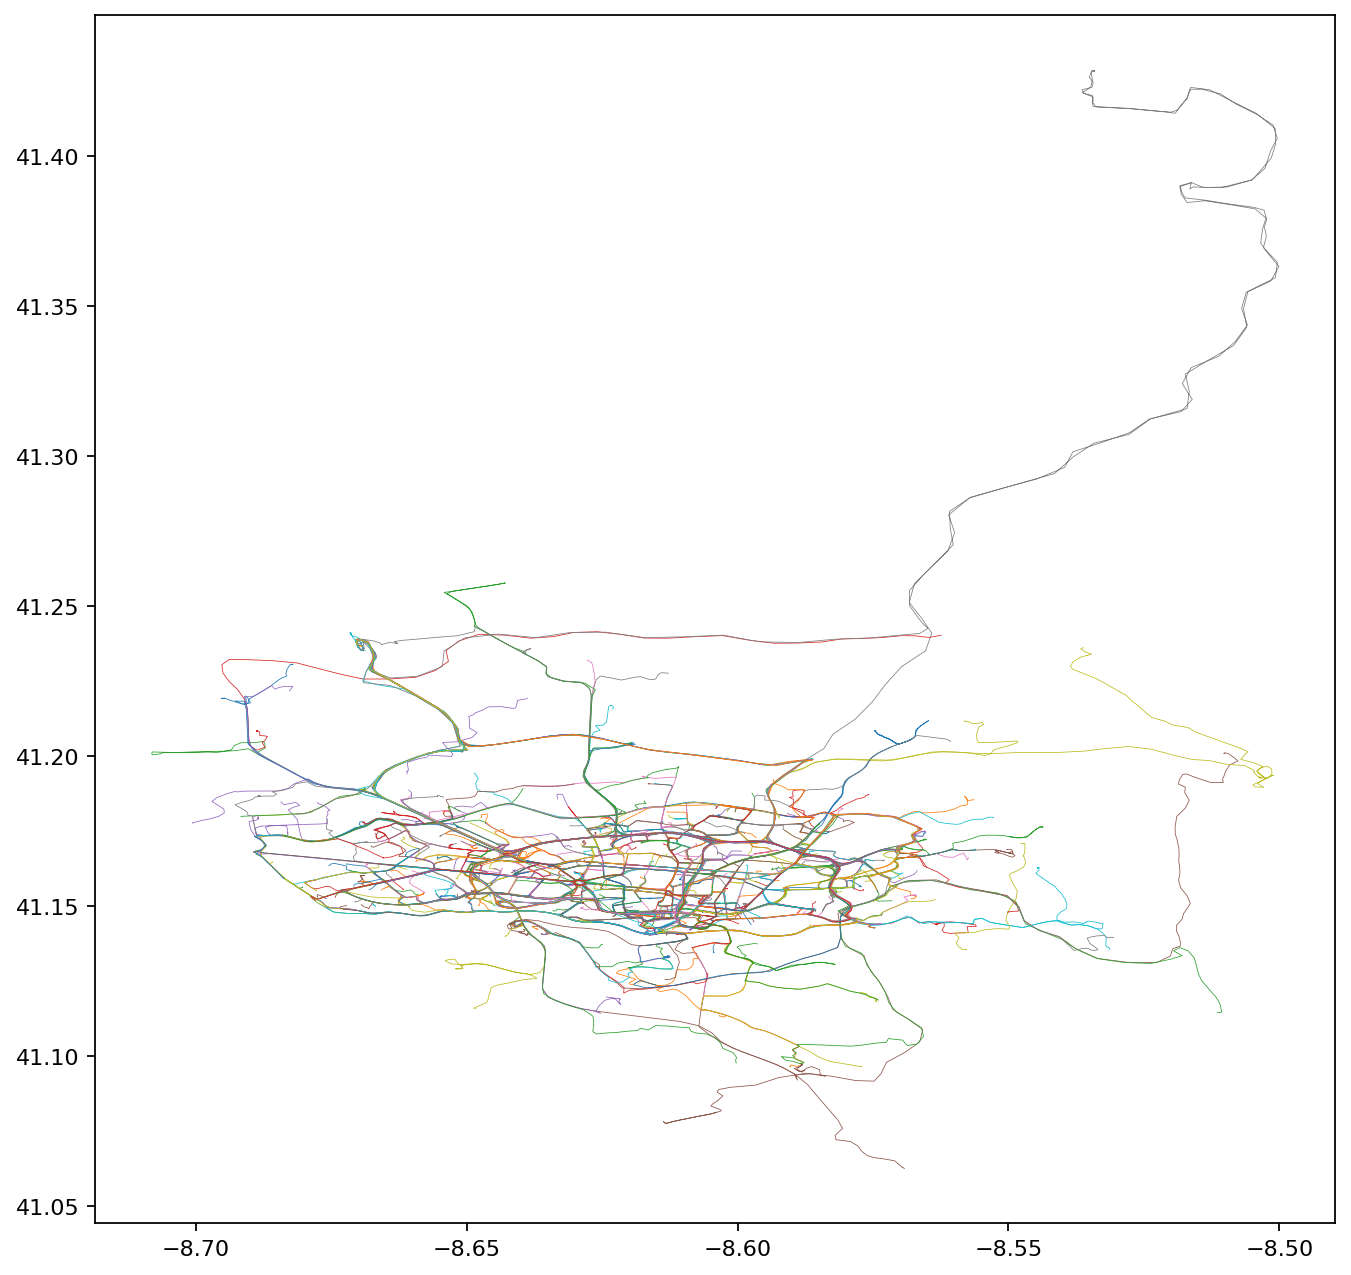
\includegraphics[width=\textwidth]{figs/traj/REAL_MED.png}
    \caption{Subset with 551 entries}
    \label{sfig:real-med}
\end{subfigure}
\hfill
\begin{subfigure}{.451\textwidth}
    \centering
    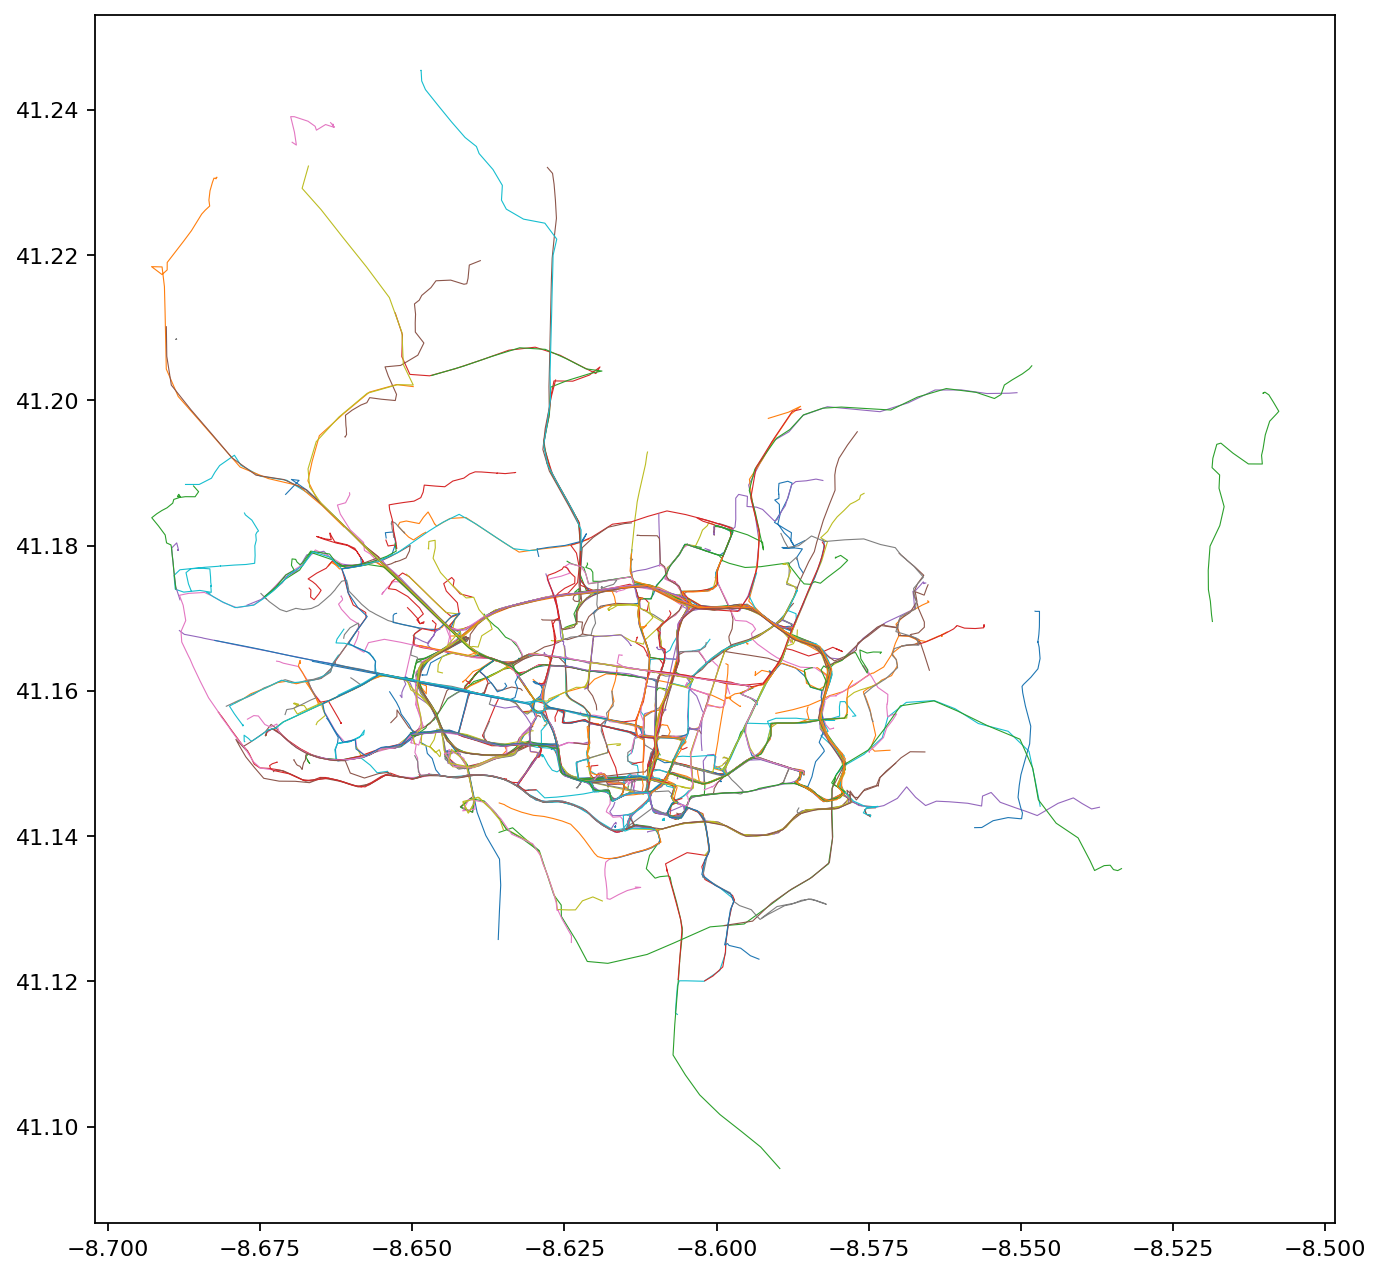
\includegraphics[width=\textwidth]{figs/traj/REAL_TRUNC.png}
    \caption{Truncated subset, 353 entries}
    \label{sfig:real-trunc}
\end{subfigure}
\begin{subfigure}{.451\textwidth}
    \centering
    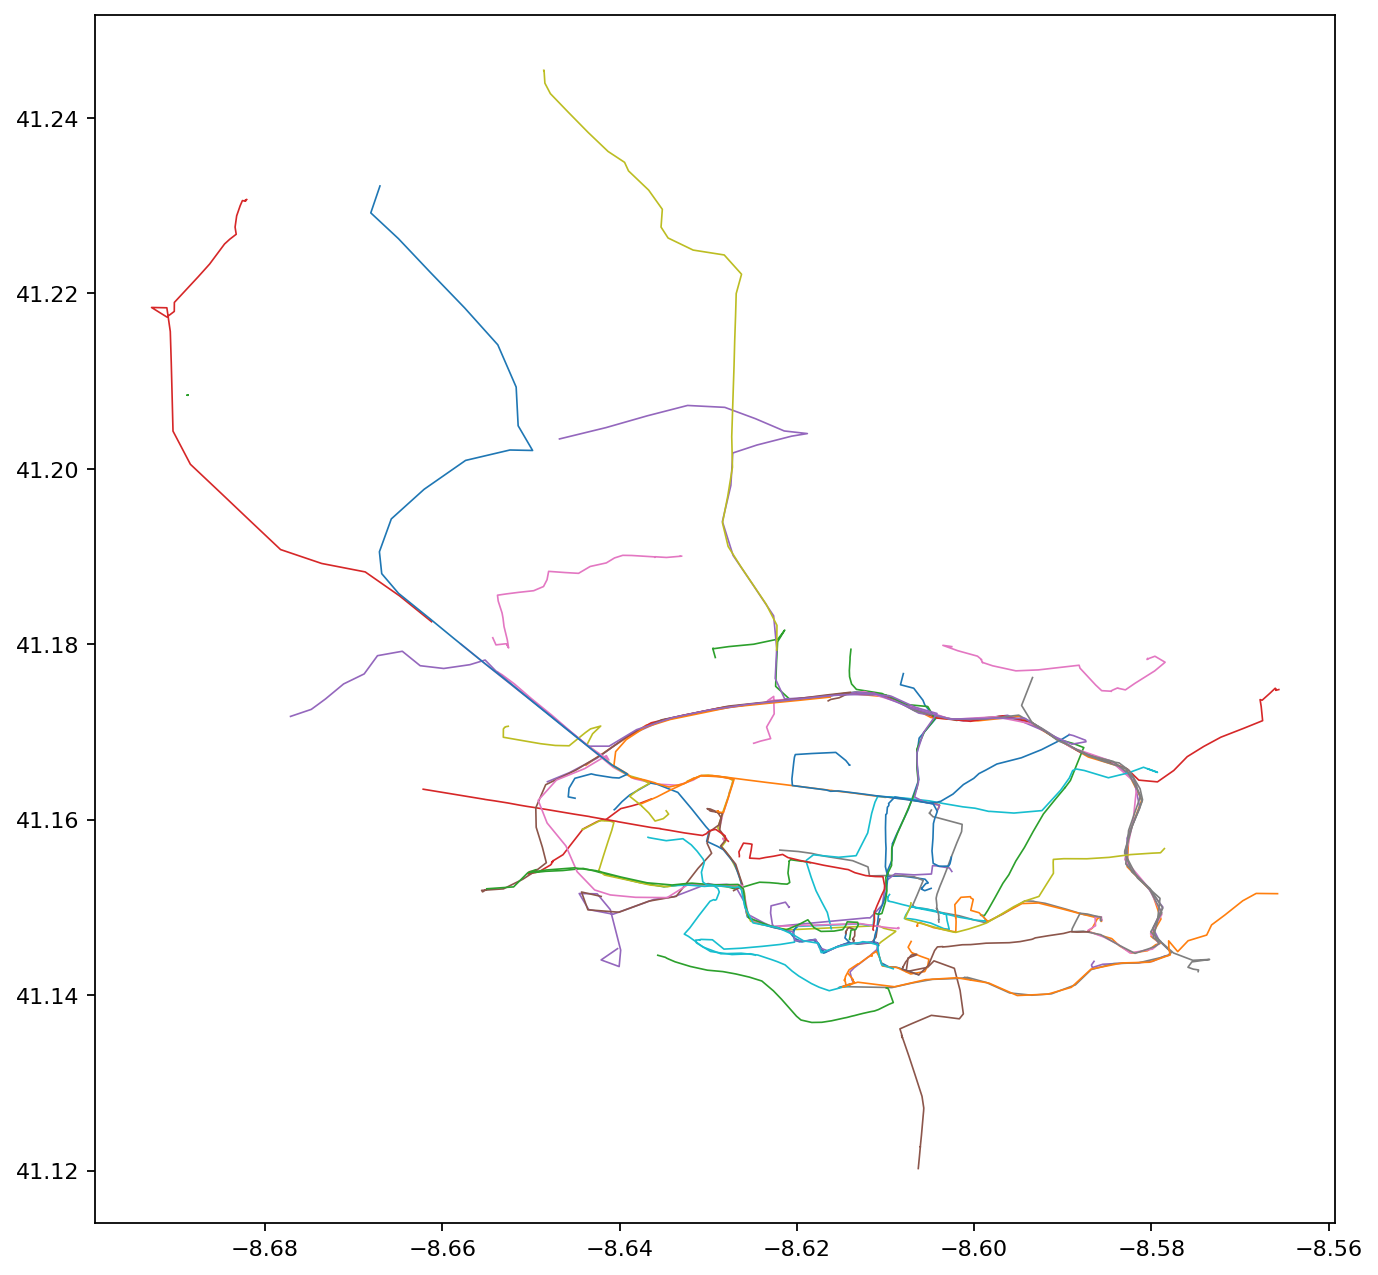
\includegraphics[width=\textwidth]{figs/traj/REAL_TRUNC_MINI.png}
    \caption{Subset of the truncated data with 53 entries}
    \label{sfig:real-trunc-mini}
\end{subfigure}
\caption{Real data set with trajectories collected from taxis}
\label{fig:real-datasets}
\end{figure}


\begin{figure}[h!]
\centering
\begin{subfigure}{.45\textwidth}
    \centering
    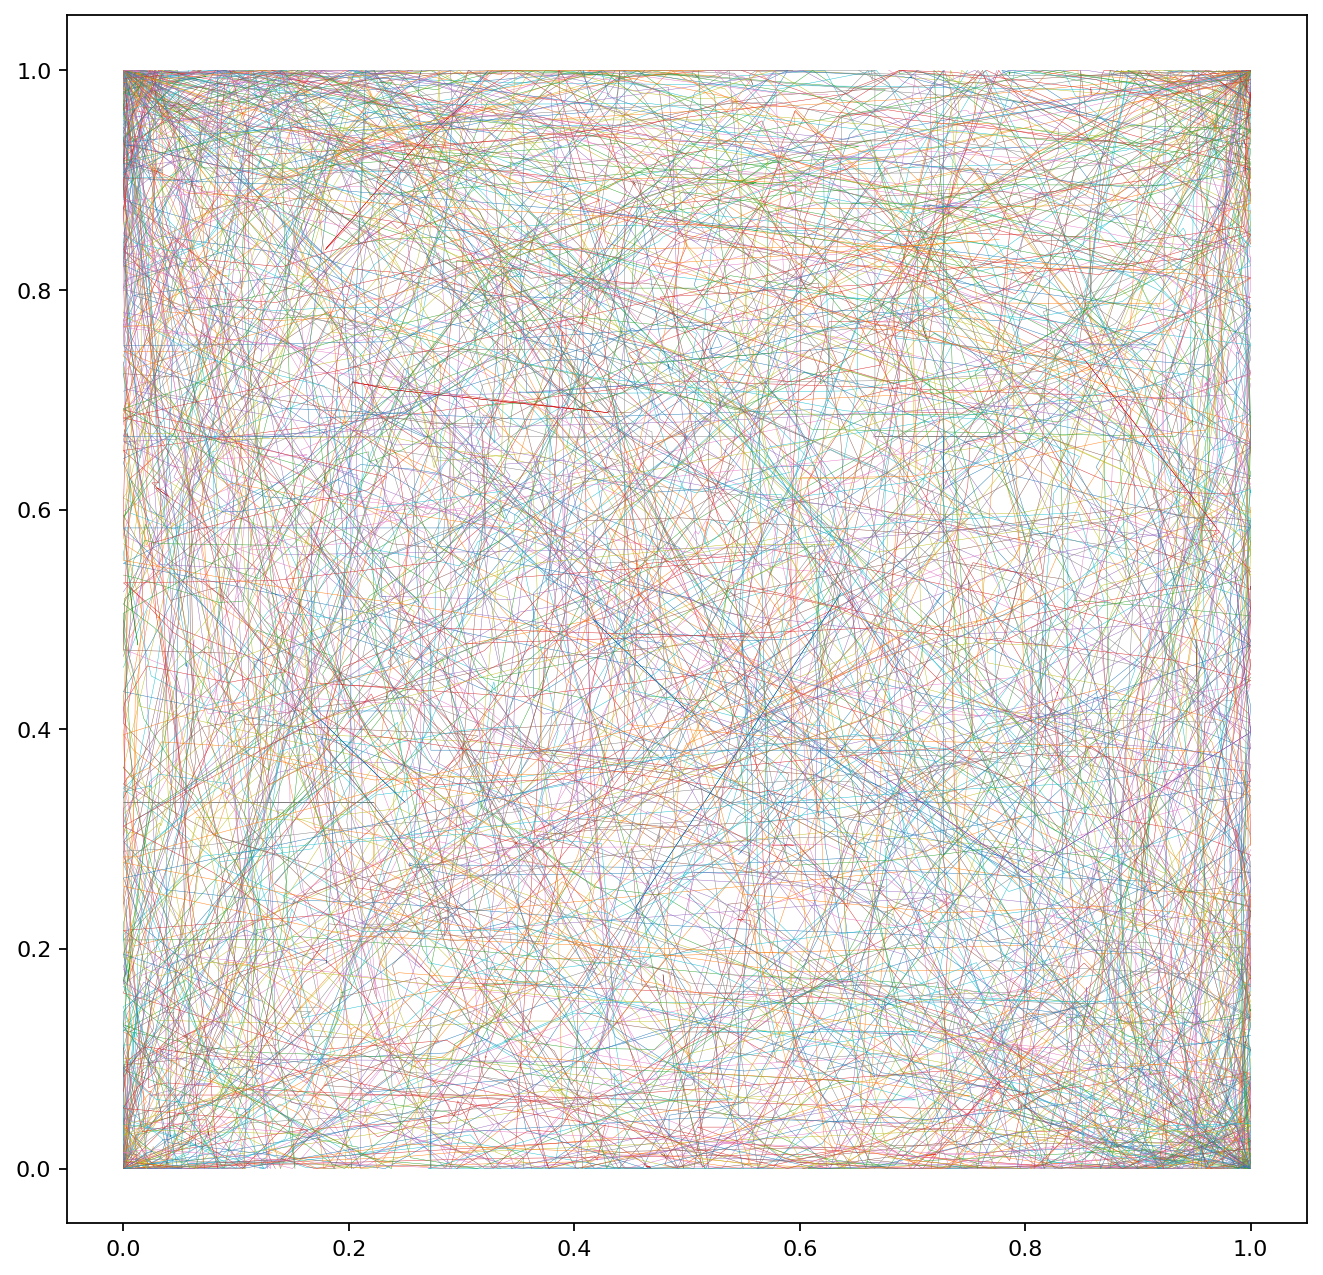
\includegraphics[width=\textwidth]{figs/traj/REAL_TRUNC_SCL.png}
    \caption{Scaled version of the data set in \newline\Cref{sfig:real-trunc}}
\end{subfigure}
\hfill
\begin{subfigure}{.45\textwidth}
    \centering
    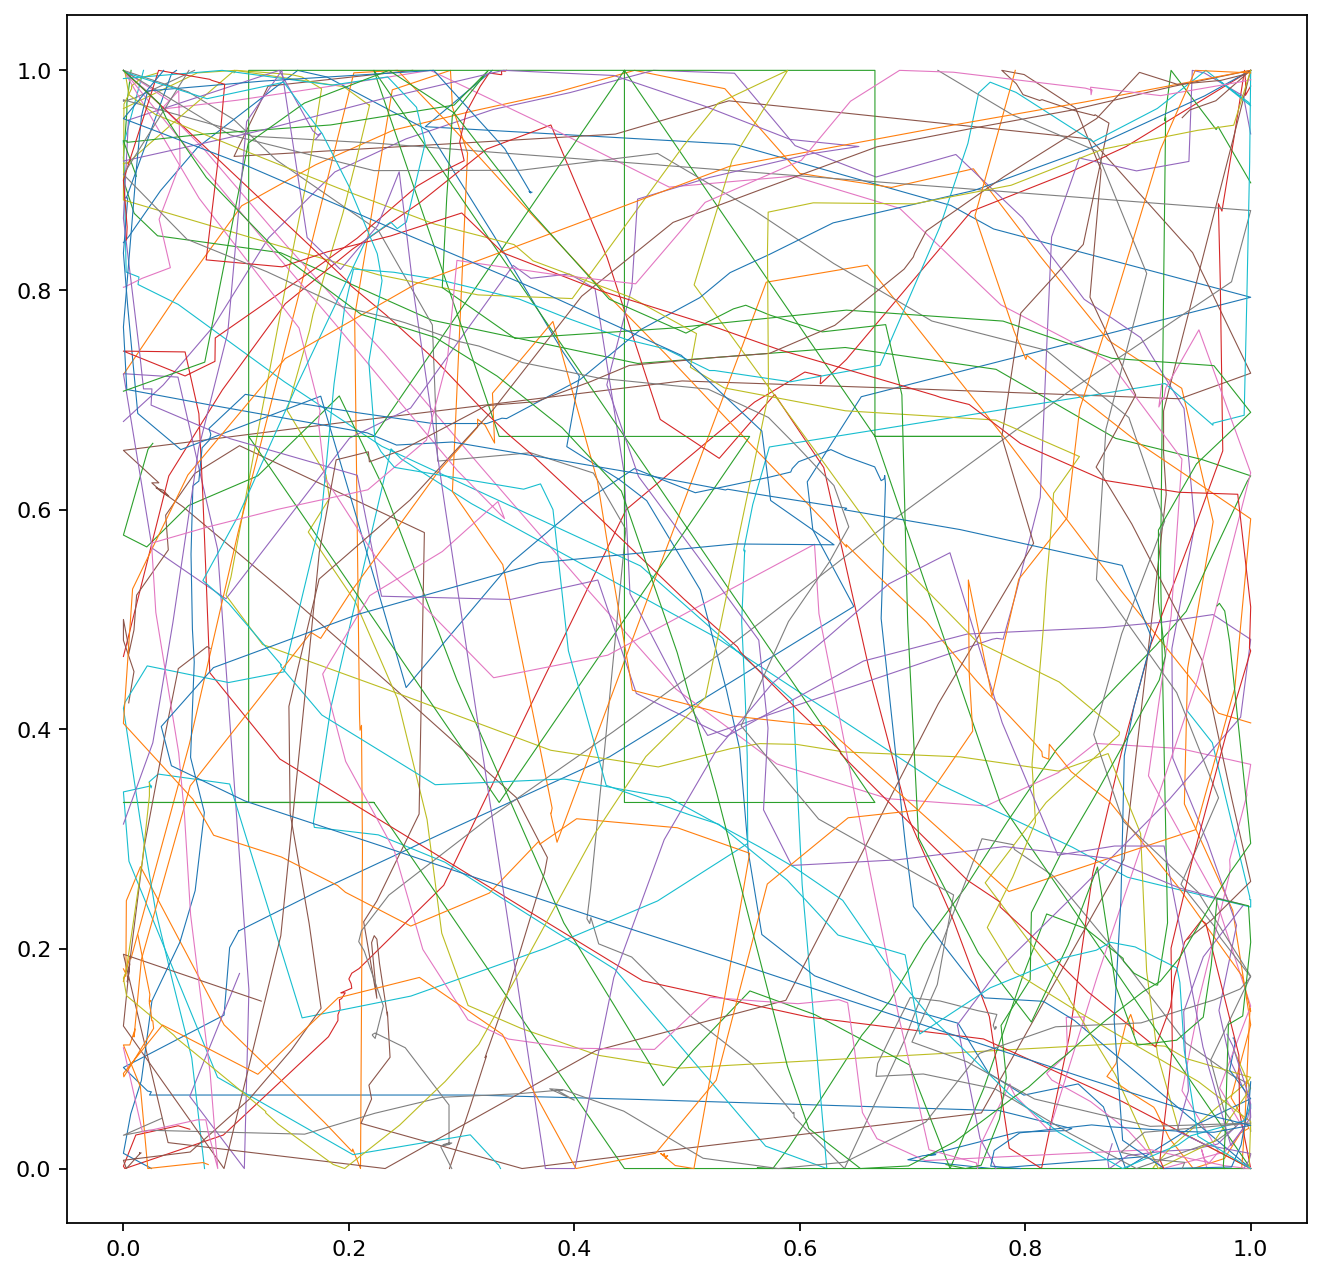
\includegraphics[width=\textwidth]{figs/traj/REAL_TRUNC_SCL_MINI.png}
    \caption{Scaled version of the data set in\newline \Cref{sfig:real-trunc-mini}}
\end{subfigure}
\caption{The trajectories in the data set after re-scaling}
\label{fig:scl-datasets}
\end{figure}



\section{Setting Parameter Values}

Three of the measures required a parameter value. 
For each of the measures, we followed the guidelines that the original creators set for determining a fitting value.
While the value may have been usable for our tests, we did not fully optimize any of the parameters for this specific data set. 
This may have negatively impacted their performance, and as a counter, we would test more than one value where we could reasonably determine another value. 
For details regarding parameters themselves, refer to \Cref{ch:2}. 


\subsection{EDR}

The creators of this method explicitly stated that they achieved the best clustering results when the matching threshold $\epsilon$ was set to a quarter of the maximum standard deviation\cite{12-RobustFast}. 
The time-series data that were used in their research were one-dimensional, thus finding the standard deviations of each series was a straightforward task.
Akin to how to how the re-scaling was done, a naive process that isolated the two dimensions was used to estimate a sensible value for $\epsilon$. 
For each trajectory, the standard deviation of each dimension was calculated.
Then the mean of the largest standard deviations from the data set was computed.
A quarter of that value was used as the first value of $\epsilon$, while the second value was half; the two values we used for EDR were $\{0.101, 0.203\}$

\clearpage
\subsection{ERP}
The researchers that developed ERP stated that the algorithm would be a metric as long as the reference value, $g$, was fixed\cite{13-MarriageLpnorms}.

In their paper, they asserted that fixing $g$ at the origin was a natural choice. 
Consequently, we set $g = (0, 0) $ for the tests in this set up. 
We did not try another value for $g$ due to there being a lack on information of how approximate another suitable value.

% em dash  –

\subsection{MSM}
Much like the creators of the algorithm– and subsequent experiments of MSM \cite{40-MoveSplitMergeMetric, 42-GreatTime, 52-OnlineEfficient}, we let the cost, $c$, vary over different orders of magnitude. 
Concretely $c$ took the values  $\{1, 0.1, 0.01\}$.
These orders of magnitude were chosen based on the results from initial tests executed on the subset of truncated trajectories.  

% \section{Condensed Similarity Matrices}
% Most of these methods were readily implemented in an existing python module \cite{43}. More about implementation in \Cref{ch:5}.


\section{Clustering Analysis}
\label{sec:5-clustering}

% All similarity distances but MSM were computed using an existing python library\cite{43-TrajectoryDistance} for trajectory similarity. In order to compute the MSM similarity distance we adapted the JAVA implementation for $1-$dimensional time-series data that its creators had published. 
The first step was to compute all pairwise trajectory similarity scores using each of the similarity distance functions. 
The next step was to create the clusters and as specified in \Cref{ch:2}  two different models were used for this. Details on the clustering models were given in that chapter as well. 

The Python's module \mintinline{Python}{sklearn} contains functionality for creating for both types of clustering, as well as models for even more options.  
The module can take parameters which affect how the model creates the clusters. An example would be setting an iteration limit for affinity propagation. 
However,  in keeping this stage of the experiment as simple as possible, all but one parameter value were kept their defaults.


The value we specified was the number of clusters that the hierarchical model should create.
This was necessary as the stopping criterion for agglomerative clustering is to have one cluster that contains all elements.
The number chosen was for all intents and purposes arbitrary, but we set it to be the least number of clusters found by affinity propagation. 
Our motivation for picking this number, and keeping it equal for all measures, was that we wanted to have clusters of meaningful sizes while still being able to spot the variances from a given measure. 

Finally, we implemented a version of the Davies-Bouldin Index. 
Again, the underlying theory is elaborated upon on \Cref{ch:2}. 
The DB-index depends on having a representative observation of each cluster. 
Commonly this is either the center of a cluster or an exemplar observation that is the one nearest to other ones. 
Unfortunately, the center of a cluster of series data does not let itself be computed easily– especially in the cases where the trajectories are of unequal length. Furthermore, determining the exemplar observation would require us to pick a similarity to be the proper one.   

Yet again simplifications were made, and the center trajectory of a cluster was set to be the series of mean positions of all trajectories in that cluster.
The mean was computed in a lock-step manner using the $L_2$-norm. 
For the similarity distance computations necessary for the DB-index calculation, the Euclidean distance was used because of if the simplest one. 




% Once the parameters had been set and the data pre-processed the condensed similarity matrices were computed. With the pairwise distance between all trajectories computed we looked into the performance of each measure by applying two different clustering tasks: affinity propagation and hierarchical agglomerative clustering. The theory of the two clustering techniques are elaborated upon in [ref CHAPTER]. Scikit and sklearn models for clustering [CITE] were used for the generation of clusters.  

												

% For the hierarchical clustering, we used sklearn [CITE]’s Agglomerative Clustering model to compute the clusters and SCIPY’s cluster hierarchy methods display them. Complete linking – using a set number of clusters. An arbitrary number of final clusters were chosen, and in this case, that number was the smallest number of clusters that were found in the affinity propagation method. 

% The number of clusters should be large enough to capture the variance of possible final clusters, yet not so large that it would hinder meaningful groupings. 



% The Davies–Bouldin index was calculated by defining “separation of clusters” and “tightness within clusters” much like the authors of\cite{50-ReviewPerspective}. See CHAPTER for more details on the index and EQ for implementation specification. 
 




\section{Simplifications}

As stated at various points throughout the chapter, we made simplifications while setting up our experiment. 
The simplifications were made in order to limit the scope, and in some cases due to the time constraints surrounding the thesis. 
We close the chapter by summarizing them below. 


\begin{itemize}

\item The trajectories were truncated to equal length and then re-scaled so that they did not remain true to their original relative location. 

\medskip
\item At several points, longitude and latitude were treated as if they were independent series. 
This becomes particularly important with respect to re-scaling and cluster evaluation.

\medskip
\item At the evaluation stage, point-point distances, and trajectory-trajectory were calculated using the Euclidean distance. 
This further exaggerated the biases of the DB-index. 

\medskip
\item Clustering itself lacks a well-defined standard, meaning it is not necessarily the most appropriate application comparison.
\medskip

% the decisions to approximate the conversion 

\end{itemize}

The effect of simplification and the importance of the cluster evaluation is further elaborated upon in \Cref{ch:7}.






\chapter{Results}
\label{ch:6}

In this chapter, we will present the results of the analysis we conducted.
First, we briefly look at how the algorithms scored the trajectories. 
For the remainder of the chapter, we focus on the clusters and meaningfully interpret them. 



\section{Similarity Scores}
Even though they lay the basis for further analysis, there is no meaningful way to directly compare the similarity scores. 
However, it could be interesting to look at their ranking of trajectory pairs. 
We are present the ten pairs that each measure deemed the most similar in \Cref{tab:top-10-sim-pairs}. 

\begin{table}[]
\centering
\caption{Overview of most similar trajectory pairs according to each measure. A larger version of the table is in\Cref{app:a-simtab}  }
\resizebox{\textwidth}{!}{%
\renewcommand{\arraystretch}{1.1}
\begin{tabular}{@{}|l|l|l|l|l|l|l|l|l|l|@{}}
\toprule
\textbf{Euclidean} &
  \textbf{DTW} &
  \textbf{SSPD} &
  \textbf{Hausdorff} &
  \textbf{ERP} &
  \textbf{MSM; cost=1} &
  \textbf{MSM; cost=.1} &
  \textbf{MSM; cost=.01} &
  \textbf{EDR; $\epsilon=.203$} &
  \textbf{EDR; $\epsilon=.101$} \\ \midrule
{\color[HTML]{CB0000} \textit{QREOR-IHNMX}} &
  {\color[HTML]{986536} \textit{LFQDH-ACJIG}} &
  {\color[HTML]{986536} \textit{LFQDH-ACJIG}} &
  {\color[HTML]{000000} WBNSL-SATNK} &
  {\color[HTML]{CB0000} \textit{QREOR-IHNMX}} &
  {\color[HTML]{CB0000} \textit{QREOR-IHNMX}} &
  {\color[HTML]{CB0000} \textit{QREOR-IHNMX}} &
  {\color[HTML]{986536} \textit{LFQDH-ACJIG}} &
  {\color[HTML]{986536} \textit{LFQDH-ACJIG}} &
  {\color[HTML]{986536} \textit{LFQDH-ACJIG}} \\
{\color[HTML]{986536} \textit{LFQDH-ACJIG}} &
  {\color[HTML]{009901} \textit{NVZCQ-TGKDX}} &
  {\color[HTML]{000000} WBNSL-SATNK} &
  {\color[HTML]{009901} \textit{NVZCQ-TGKDX}} &
  {\color[HTML]{986536} \textit{LFQDH-ACJIG}} &
  {\color[HTML]{986536} \textit{LFQDH-ACJIG}} &
  {\color[HTML]{986536} \textit{LFQDH-ACJIG}} &
  {\color[HTML]{009901} \textit{NVZCQ-TGKDX}} &
  {\color[HTML]{000000} LVFYZ-LENWX} &
  {\color[HTML]{CB0000} \textit{QREOR-IHNMX}} \\
{\color[HTML]{000000} BZCYT-VXLBC} &
  {\color[HTML]{CB0000} \textit{QREOR-IHNMX}} &
  {\color[HTML]{000000} KQQUG-OVNBK} &
  {\color[HTML]{000000} NHNMB-PSVVR} &
  {\color[HTML]{000000} BZCYT-VXLBC} &
  {\color[HTML]{000000} BZCYT-VXLBC} &
  {\color[HTML]{009901} \textit{NVZCQ-TGKDX}} &
  {\color[HTML]{000000} KQQUG-OVNBK} &
  {\color[HTML]{000000} XXVQK-LOBQA} &
  {\color[HTML]{000000} KQQUG-OVNBK} \\
{\color[HTML]{3531FF} \textit{LHTXJ-TGKDX}} &
  {\color[HTML]{000000} HXVAH-RPCOW} &
  {\color[HTML]{CB0000} \textit{QREOR-IHNMX}} &
  {\color[HTML]{000000} HXVAH-RPCOW} &
  {\color[HTML]{3531FF} \textit{LHTXJ-TGKDX}} &
  {\color[HTML]{3531FF} \textit{LHTXJ-TGKDX}} &
  {\color[HTML]{000000} BZCYT-VXLBC} &
  {\color[HTML]{000000} WBNSL-SATNK} &
  {\color[HTML]{000000} BLHVW-ATPTV} &
  {\color[HTML]{000000} LFQDH-ASYEZ} \\
{\color[HTML]{000000} PSVVR-XSJJE} &
  {\color[HTML]{000000} KQQUG-OVNBK} &
  {\color[HTML]{000000} NHNMB-PSVVR} &
  {\color[HTML]{CB0000} \textit{QREOR-IHNMX}} &
  {\color[HTML]{000000} PSVVR-XSJJE} &
  {\color[HTML]{000000} PSVVR-XSJJE} &
  {\color[HTML]{000000} KQQUG-OVNBK} &
  {\color[HTML]{CB0000} \textit{QREOR-IHNMX}} &
  {\color[HTML]{000000} WBTAG-QMRPP} &
  {\color[HTML]{009901} \textit{NVZCQ-TGKDX}} \\
{\color[HTML]{009901} \textit{NVZCQ-TGKDX}} &
  {\color[HTML]{000000} JRDIM-OVNBK} &
  {\color[HTML]{009901} NVZCQ-TGKDX} &
  {\color[HTML]{000000} JRDIM-OVNBK} &
  {\color[HTML]{009901} \textit{NVZCQ-TGKDX}} &
  {\color[HTML]{009901} \textit{NVZCQ-TGKDX}} &
  {\color[HTML]{000000} LFQDH-ASYEZ} &
  {\color[HTML]{000000} HXVAH-RPCOW} &
  {\color[HTML]{000000} NKEGR-VXLBC} &
  {\color[HTML]{000000} BZCYT-VXLBC} \\
{\color[HTML]{000000} TNPJQ-LRZLR} &
  {\color[HTML]{000000} WBNSL-SATNK} &
  {\color[HTML]{000000} HXVAH-RPCOW} &
  {\color[HTML]{986536} \textit{LFQDH-ACJIG}} &
  {\color[HTML]{000000} TNPJQ-LRZLR} &
  {\color[HTML]{000000} TNPJQ-LRZLR} &
  {\color[HTML]{3531FF} \textit{LHTXJ-TGKDX}} &
  {\color[HTML]{3531FF} \textit{LHTXJ-TGKDX}} &
  {\color[HTML]{000000} TNPJQ-LRZLR} &
  {\color[HTML]{000000} PSVVR-XSJJE} \\
{\color[HTML]{000000} HUSJF-UHLAI} &
  {\color[HTML]{000000} NHNMB-PSVVR} &
  {\color[HTML]{000000} JRDIM-OVNBK} &
  {\color[HTML]{000000} KQQUG-OVNBK} &
  {\color[HTML]{000000} HUSJF-UHLAI} &
  {\color[HTML]{000000} HUSJF-UHLAI} &
  {\color[HTML]{000000} PSVVR-XSJJE} &
  {\color[HTML]{000000} JRDIM-OVNBK} &
  {\color[HTML]{000000} PSVVR-XSJJE} &
  {\color[HTML]{000000} KQQUG-GRPNX} \\
{\color[HTML]{000000} ZQZSA-NVZCQ} &
  {\color[HTML]{3531FF} \textit{LHTXJ-TGKDX}} &
  {\color[HTML]{3531FF} \textit{LHTXJ-TGKDX}} &
  {\color[HTML]{000000} DADNP-LOBQA} &
  {\color[HTML]{000000} ZQZSA-NVZCQ} &
  {\color[HTML]{000000} ZQZSA-NVZCQ} &
  {\color[HTML]{000000} HXVAH-RPCOW} &
  {\color[HTML]{000000} LFQDH-ASYEZ} &
  {\color[HTML]{3531FF} \textit{LHTXJ-TGKDX}} &
  {\color[HTML]{000000} CWCGU-ACJIG} \\
{\color[HTML]{000000} NVZCQ-TNPJQ} &
  {\color[HTML]{000000} BZCYT-VXLBC} &
  {\color[HTML]{000000} SATNK-FIVOK} &
  {\color[HTML]{000000} OAAYX-OKPGU} &
  {\color[HTML]{000000} NVZCQ-TNPJQ} &
  {\color[HTML]{000000} NVZCQ-TNPJQ} &
  {\color[HTML]{000000} HUSJF-UHLAI} &
  {\color[HTML]{000000} NHNMB-PSVVR} &
  {\color[HTML]{000000} HUSJF-UHLAI} &
  {\color[HTML]{000000} EBYMF-LENWX} \\ \midrule
\end{tabular}
}
\label{tab:top-10-sim-pairs}
\end{table}


We observe that there is variance with respect to where the pairs are placed, yet there are a handful of recurrent pairs.
We noticed that one of the trajectory pairs appeared in the top-10 ranks for all the measures. 
Furthermore, two pairs appeared for all but one measure, and one pair that was in all but two. 
These four frequent pairs have been highlighted in \Cref{tab:top-10-sim-pairs} and are displayed in \Cref{fig:most_common_pairs}. 
The table has 27 distinct trajectory pairs, indicating that the measures generally agree on which pairs are the most similar ones. 

\begin{figure}[ht]
  \centering
  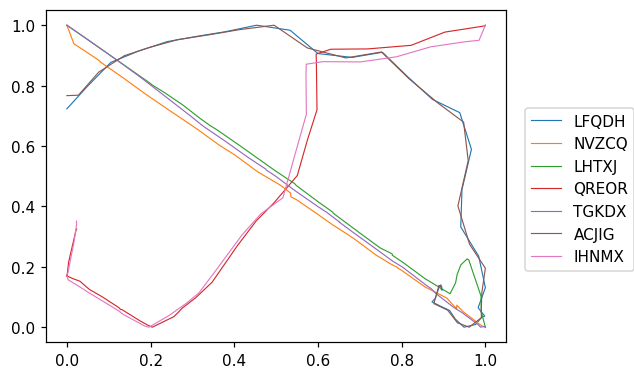
\includegraphics[width=.6\linewidth]{figs/traj/4_most_common.png}
  %    \begin{subfigure}[c]{0.35\linewidth}
  \caption{The trajectory pairs that appeared the most based on the similarity scores. }
  \label{fig:most_common_pairs}
\end{figure}




% in FIGURE the trajectories of the pairs that were the most frequent is shown. The left side has is the re-scaled tracks and the right ones is the raw GPS data.   


% \begin{table}[tbp]
%   \centering
%   \caption{Table of the top 10 most similar trajectory pairs}
%   \label{tab:top10}
%   \csvautobooktabular{csvtables/ageiq.csv}
% %   \csvautobooktabular{csvtables/TOP_10_ALL.csv}
% \end{table}


\section{Davies-Bouldin Index}

In \Cref{tab:cluster-dbidx} we have presented the Davies-Bouldin results for each cluster per type of clustering method. 
As was brought up in \Cref{ch:5} and further elaborated upon in \Cref{ch:7}, this is not a decisive ranking.


Three observations stand out in \Cref{tab:cluster-dbidx}.
Firstly, we note that SSPD and HD have received the worst ranks under both AP and HCA. 
Next, we remarked that Ed and MSM- which had identical rankings of trajectory pair, also got the same DB-index under both types of clustering.
ERP,  which also had an identical top-10 raking, received a DB-index under AP-clustering, but did so under HCA. 
The last thing that stands out is that the HCA gave a worse result for almost all methods, except for DTW and MSM with the lowest cost value. The difference is not significant, but it is consistent.


\begin{table}[h!]
\centering
\caption{Davies-Bouldin Indices for each cluster result and how each algorithm rank against each other according to this evaluation  }
\renewcommand{\arraystretch}{1.1}
\begin{tabular}{|c|	c|c|c|c|} 
\cline{2-5}
\multicolumn{1}{c|}{} & \multicolumn{2}{c|}{\textbf{Affinity Propagation}} & \multicolumn{2}{c|}{\textbf{Hierarchical Clustering}}  \\ 
\cline{2-5}
\multicolumn{1}{c|}{} & \textit{Score} & \textit{Rank}  & \textit{Score} & \textit{Rank}     \\ 
\hline
\textbf{Ed}           & 0.091 & 3    & 0.095 & 2        \\ 
\hline
\textbf{DTW}          & 0.156 & 8    & 0.140 & 5        \\ 
\hline
\textbf{Hd}           & 0.294 & 9    & 0.459 & 9        \\ 
\hline
\textbf{SSPD}         & 0.431 & 10   & 0.531 & 10       \\ 
\hline
\textbf{ERP}    & 0.083 & 2    & 0.090 & 1        \\ 
\hline
\textbf{EDR} $\epsilon=0.203$  & 0.082 & 1    & 0.162 & 6        \\ 
\hline
\textbf{EDR} $\epsilon=0.101$  & 0.091 & 3    & 0.217 & 7        \\ 
\hline
\textbf{MSM} cost$=0.01$   & 0.150 & 6    & 0.137 & 4        \\ 
\hline
\textbf{MSM} cost$=0.1$    & 0.155 & 7    & 0.222 & 8        \\ 
\hline
\textbf{MSM} cost$=1$      & 0.091 & 3    & 0.095 & 2        \\
\hline
\end{tabular}
\label{tab:cluster-dbidx}
\end{table}



\section{Clustering}

We restate that the area of interest for this thesis is the similarity distance measures and not various clustering techniques. 
The clusters are presented grouped by how they evaluated the trajectories' similarity, or by the underlying idea trajectory similarity. 

The two models used to create the clusters will be presented alongside each other.
The number of clusters produced under affinity propagation varied from 23 to 48, and as explained in \Cref{ch:5} the number of hierarchical clusters was set to 23 for all measures. See \Cref{app:ap-clu,app:h-clu} for higher resolution depictions of all clusters. 


The first three measures’ clusters we present are the ones with the identical ranking of most similar trajectory pairs;
Euclidean distance, ERP, and MSM with cost parameter to 1. The clusters are depicted in \Cref{fig:cluster-ed-erp-msm}. Next, \Cref{fig:cluster-msm} displays the clusters obtained from the remaining parameter values of Move-Split-Merge.
Continuing with the parameters measured, \Cref{fig:cluster-edr} shows the clusters that EDR generated with both parameter values. 
Finally, \Cref{fig:cluster-dtw-hd-sspd} shows the rest of the measures, namely clusters created with DTW, Hausdorff distance, and SSPD.



\begin{figure}[h]
  \centering
  \begin{subfigure}[c]{0.3\linewidth}
    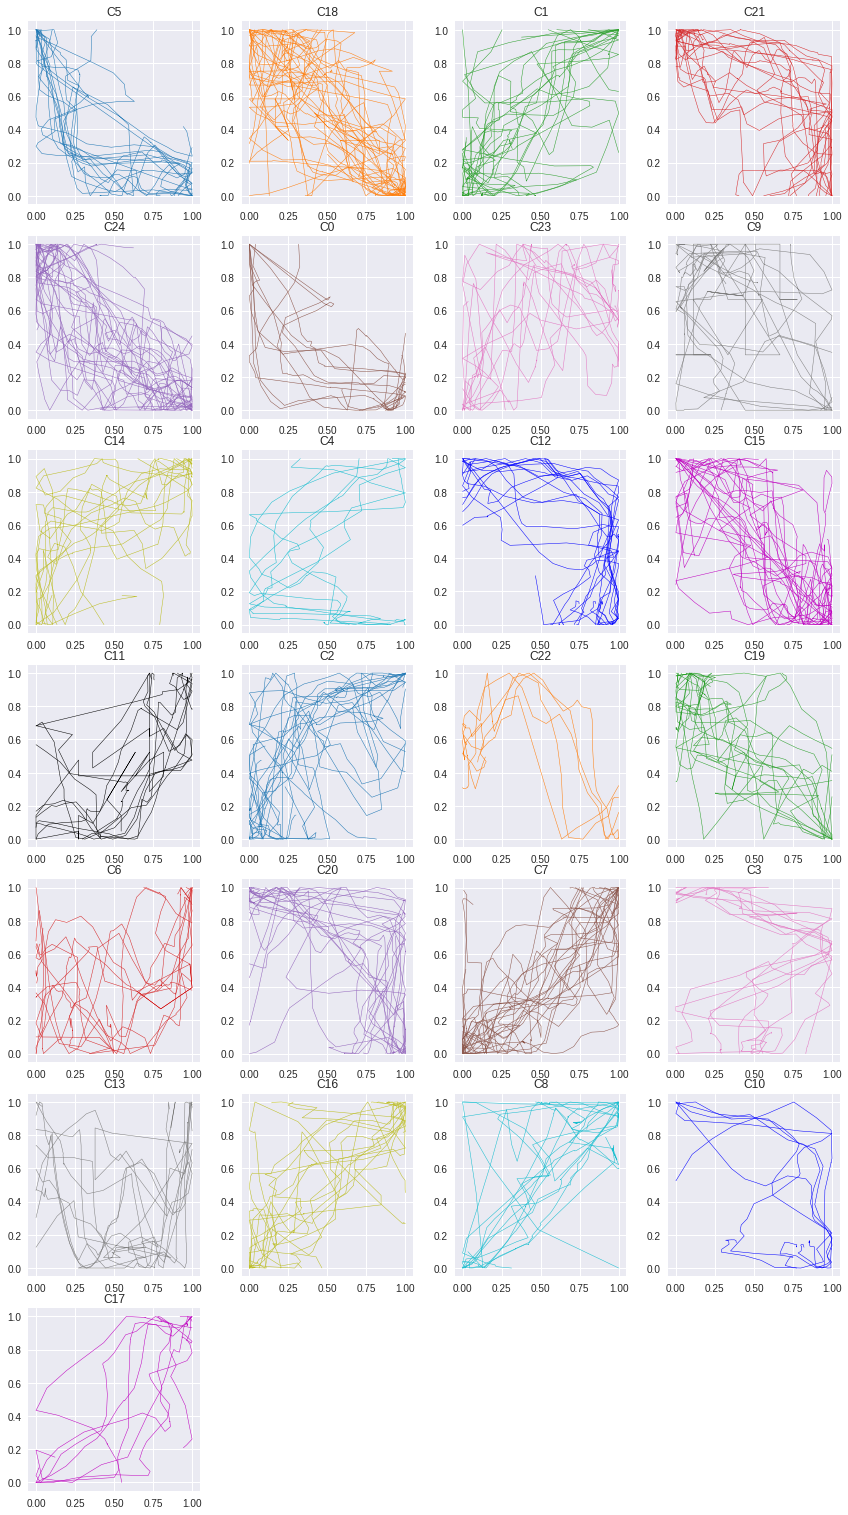
\includegraphics[width=\linewidth]{figs/clusters/CLU_AP_ALL[Ed].png}
    \caption{Euclidean}
  \end{subfigure}
  \hspace{.5em}
   \begin{subfigure}[c]{0.3\linewidth}
     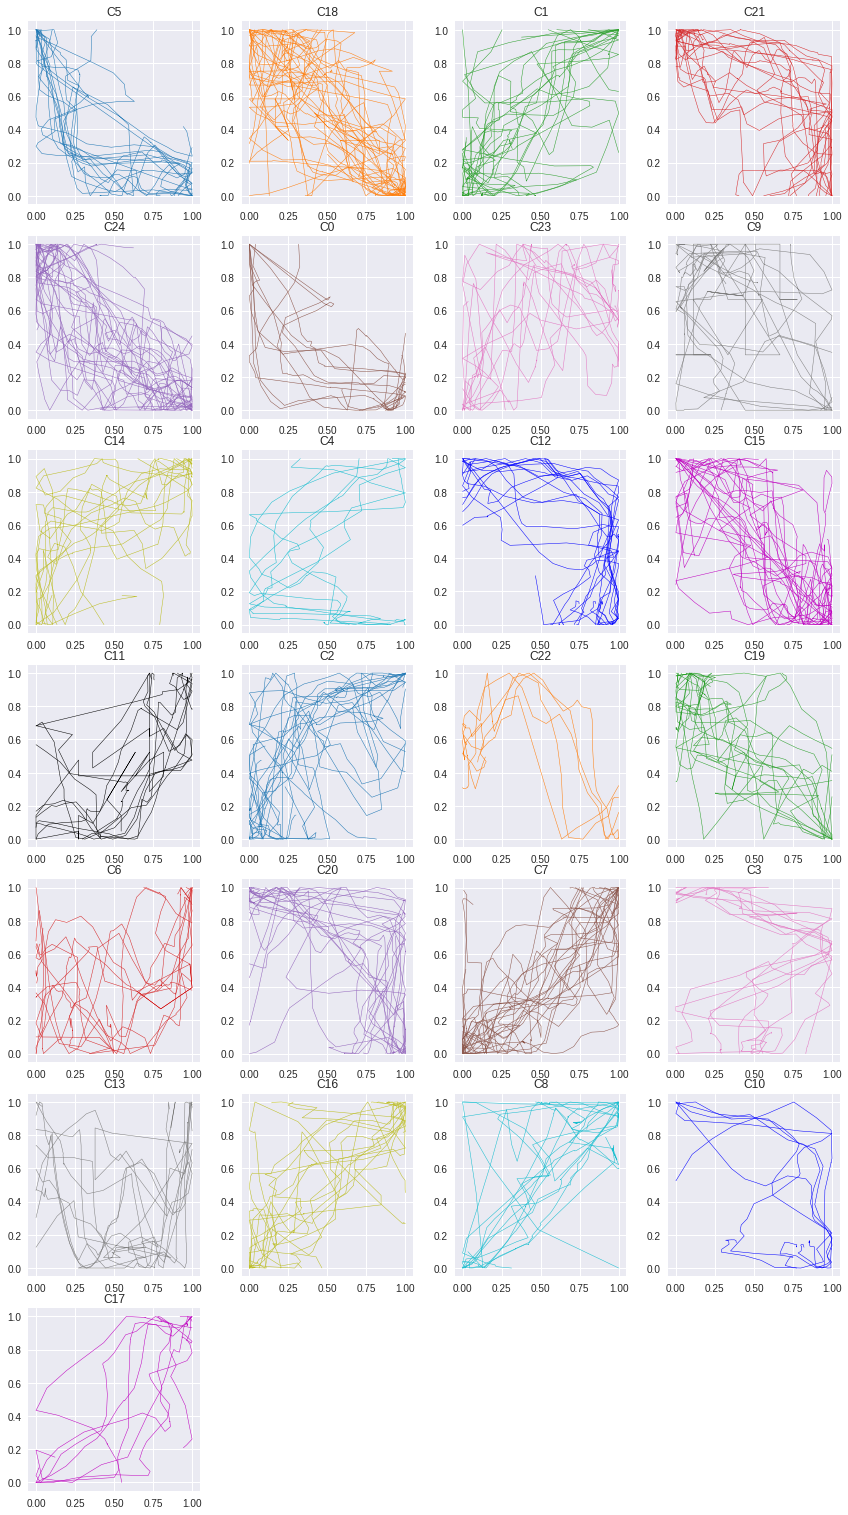
\includegraphics[width=\linewidth]{figs/clusters/CLU_AP_ALL[MSM;c=1].png}
    \caption{MSM; cost=1}
  \end{subfigure}
  \hspace{.5em}
    \begin{subfigure}[c]{0.3\linewidth}
     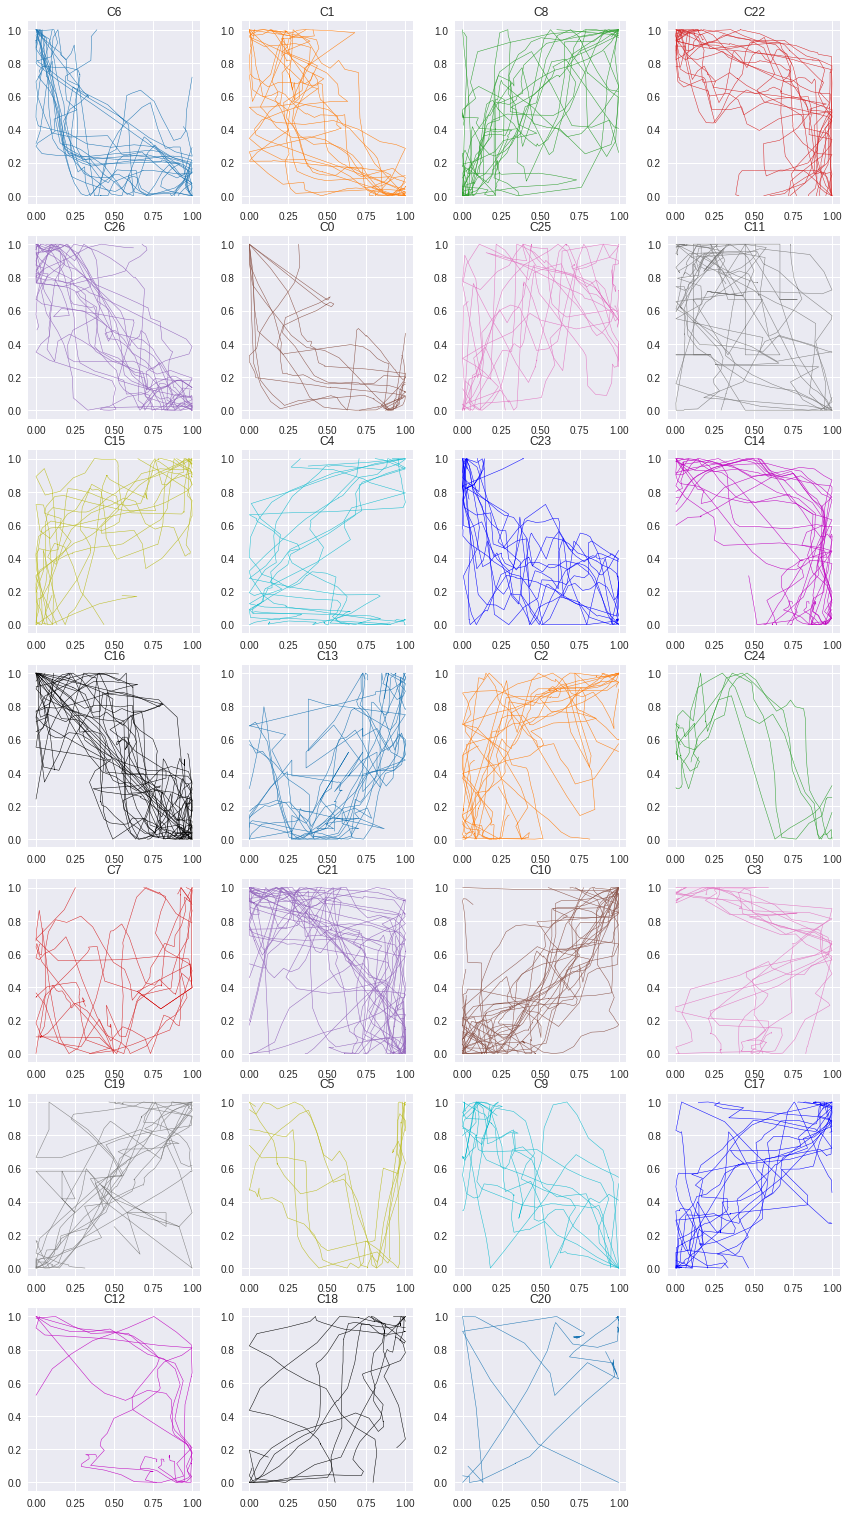
\includegraphics[width=\linewidth]{figs/clusters/CLU_AP_ALL[ERP;g=0,0].png}
    \caption{ERP}
  \end{subfigure}
  \hspace{.5em}
  
  \begin{subfigure}[c]{0.3\linewidth}
    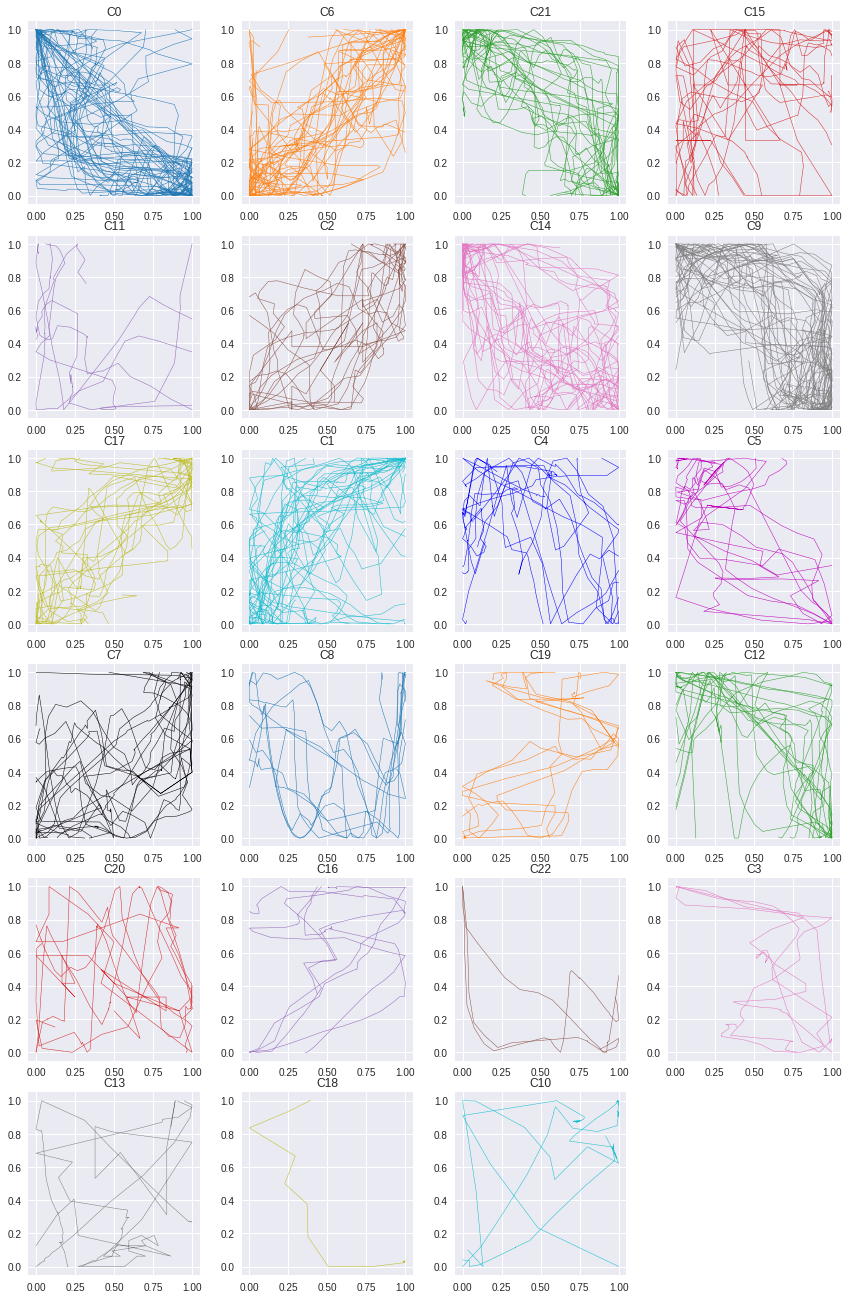
\includegraphics[width=\linewidth]{figs/clusters/CLU_H_ALL[Ed].png}
    \caption{Euclidean}
  \end{subfigure}
  \hspace{.5em}
   \begin{subfigure}[c]{0.3\linewidth}
     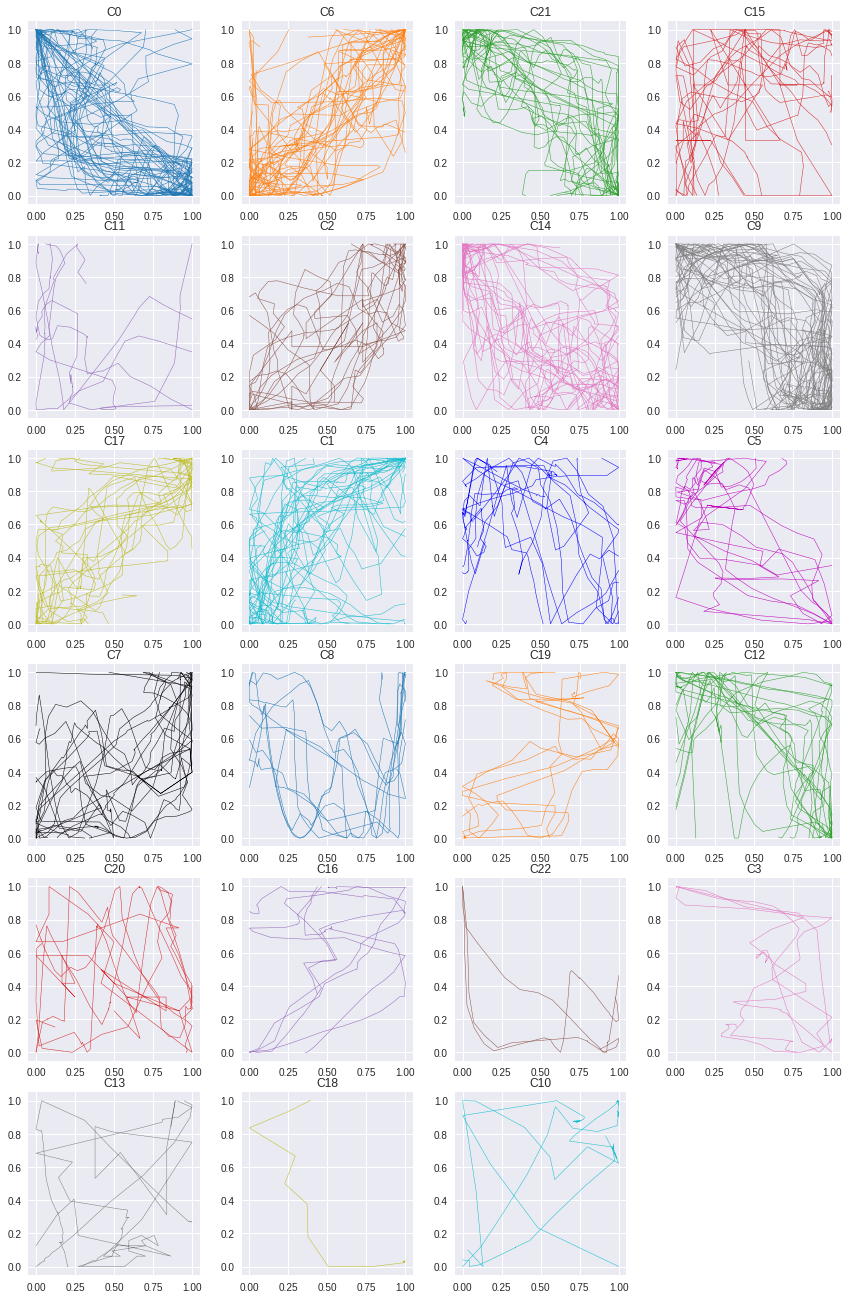
\includegraphics[width=\linewidth]{figs/clusters/CLU_H_ALL[MSM;c=1].png}
    \caption{MSM; cost=1}
  \end{subfigure}
  \hspace{.5em}
    \begin{subfigure}[c]{0.3\linewidth}
     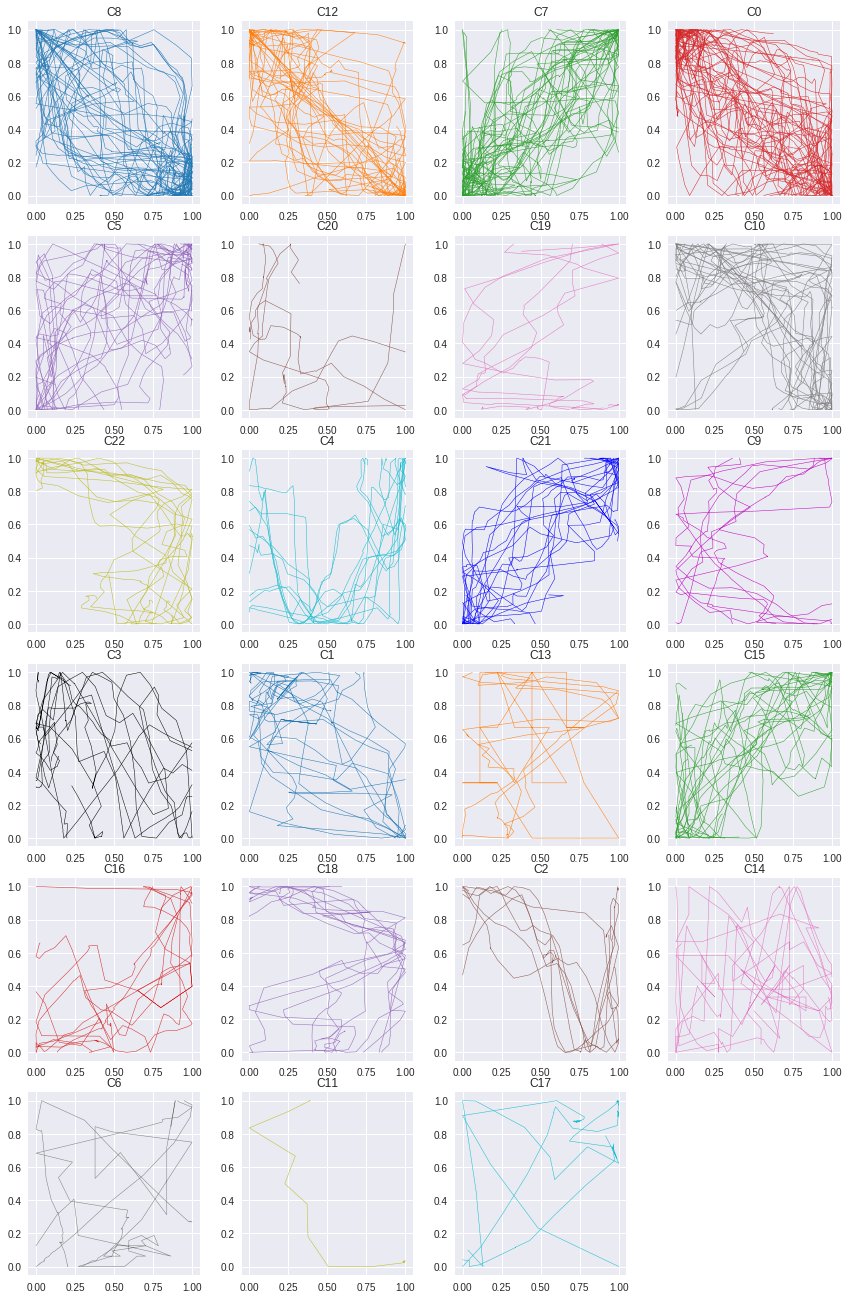
\includegraphics[width=\linewidth]{figs/clusters/CLU_H_ALL[ERP;g=0,0].png}
    \caption{ERP}
  \end{subfigure}
  \caption{Clusters of the measures that had the same raking of most similar pairs. The top row is the affinity propagation Clusters and the bottom ones are from hierarchical clustering}
  \label{fig:cluster-ed-erp-msm}
\end{figure}



\begin{figure}[h]
  \centering
  \hspace{.5em}
   \begin{subfigure}[c]{0.35\linewidth}
     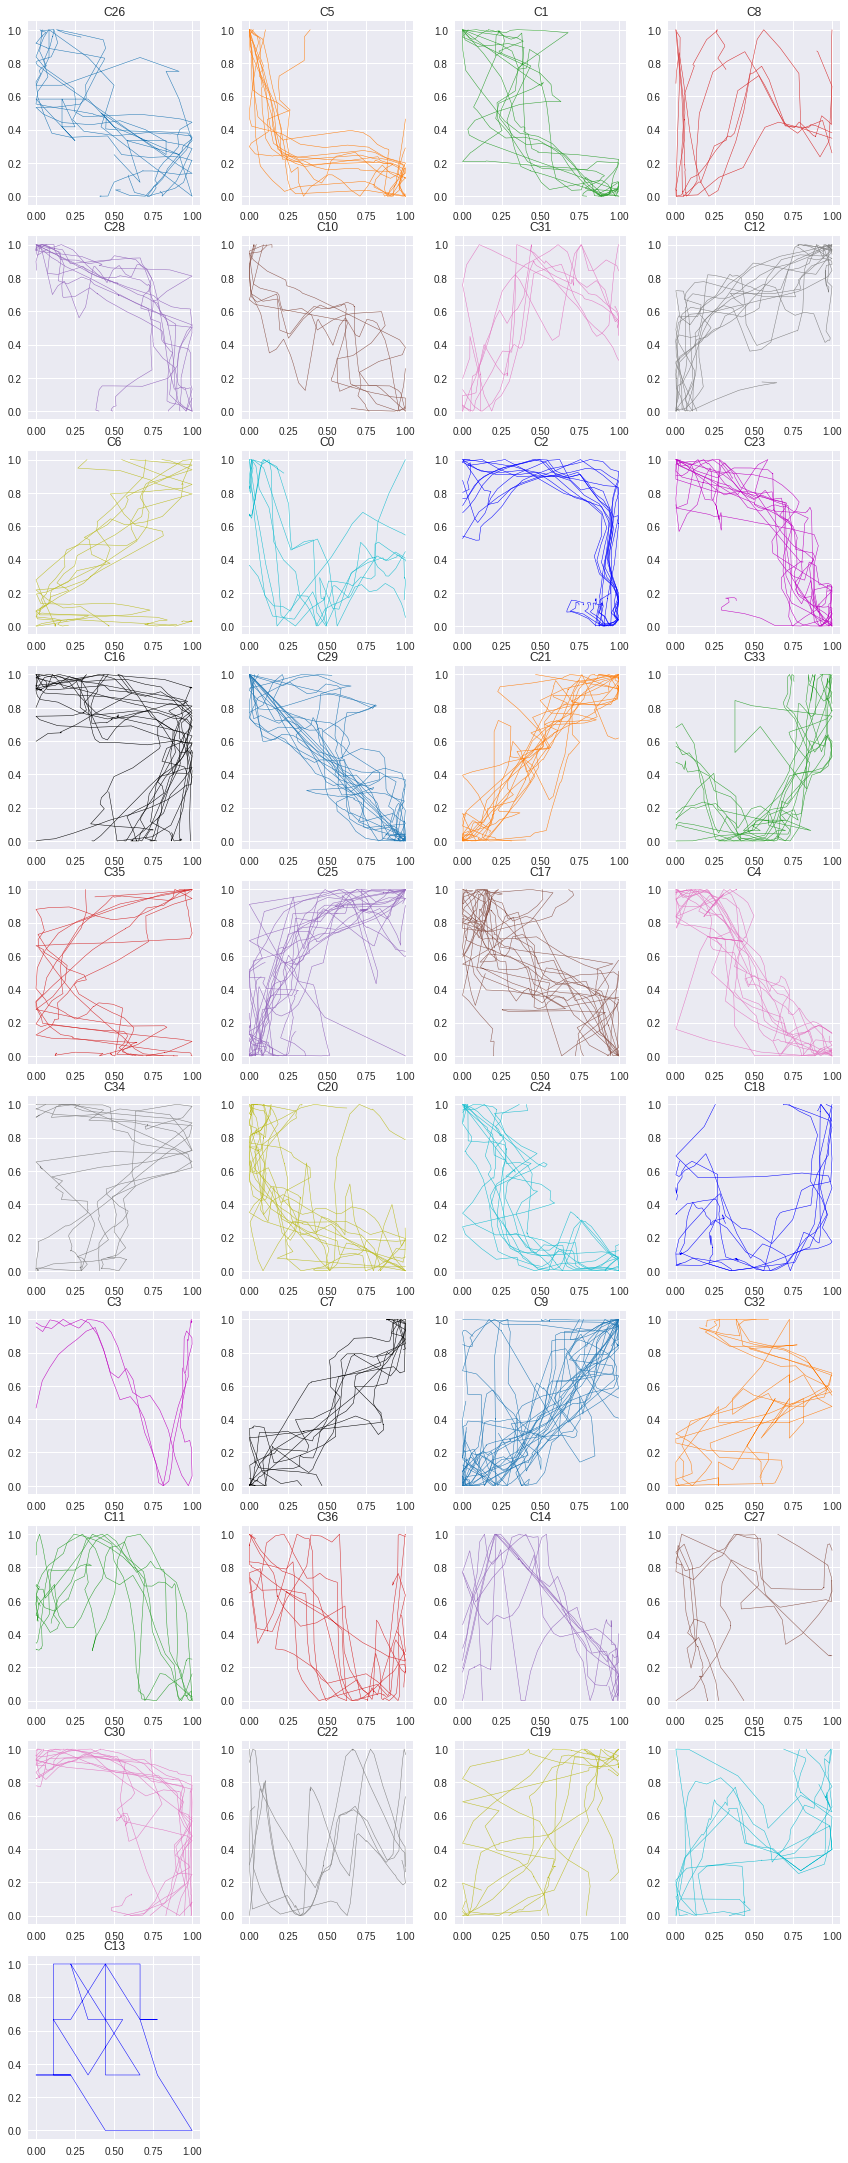
\includegraphics[width=\linewidth]{figs/clusters/CLU_AP_ALL[MSM;c=.1].png}
    \caption{MSM; Cost = 0.1}
  \end{subfigure}
  \hspace{.5em}
    \begin{subfigure}[c]{0.35\linewidth}
      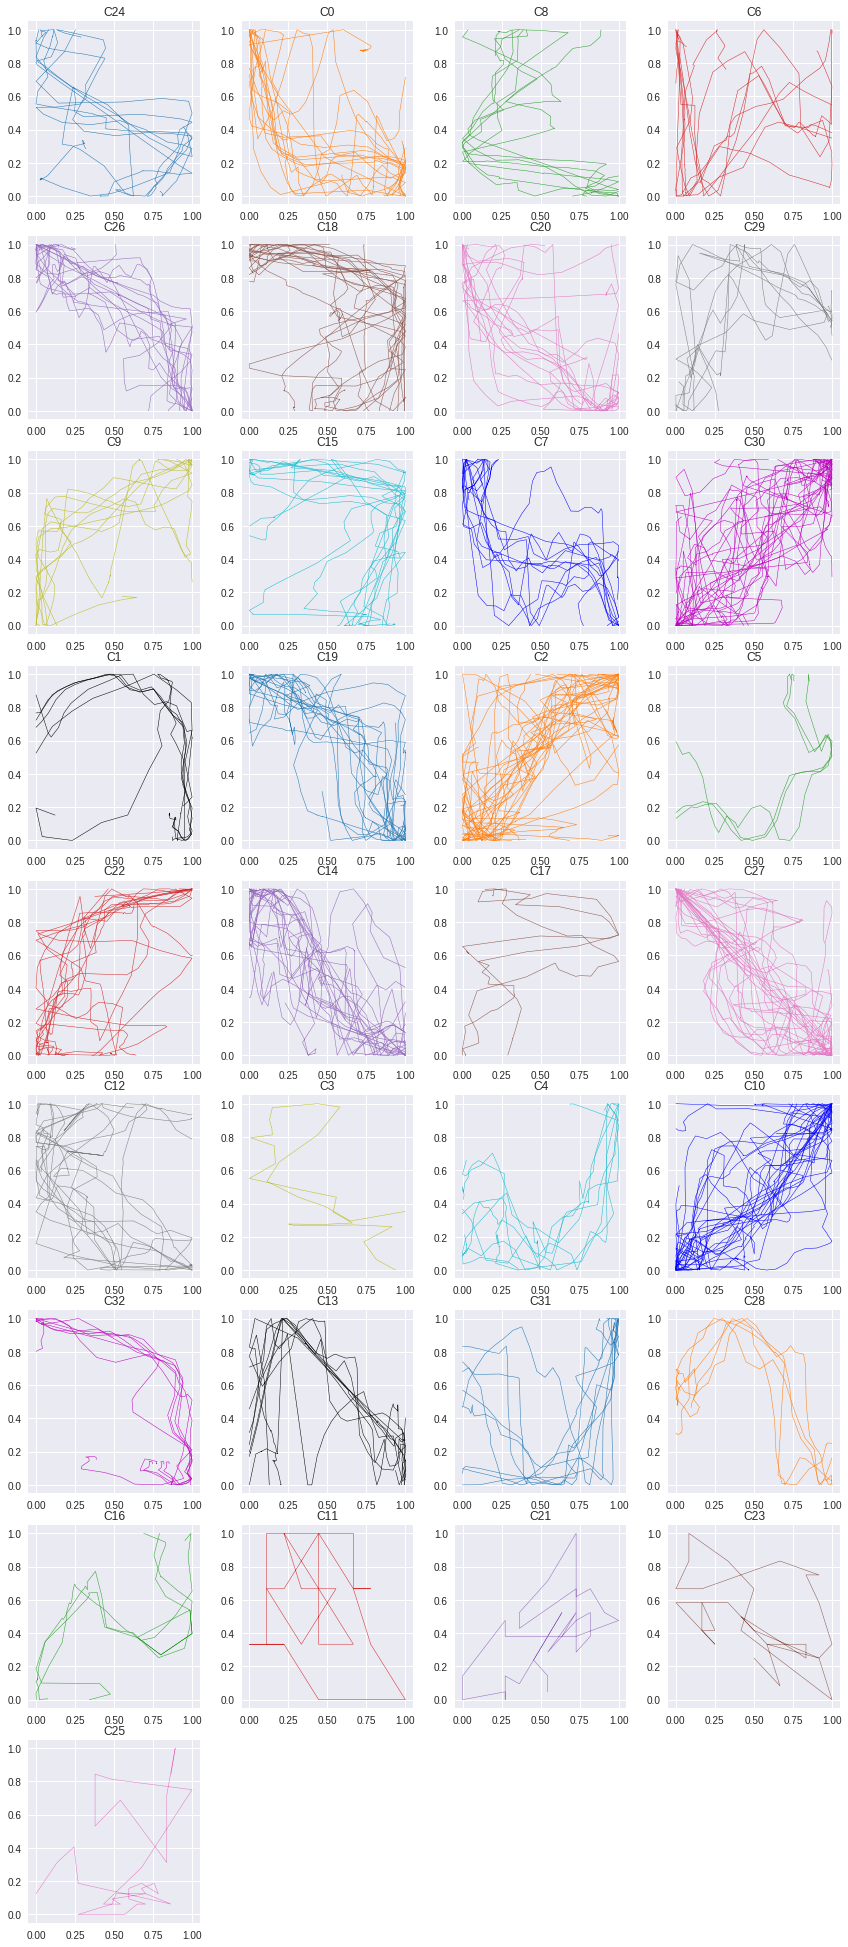
\includegraphics[width=\linewidth]{figs/clusters/CLU_AP_ALL[MSM;c=.01].png}
    \caption{MSM; Cost = 0.01}
  \end{subfigure}
  \hspace{.5em}
  
  \begin{subfigure}[c]{0.35\linewidth}
     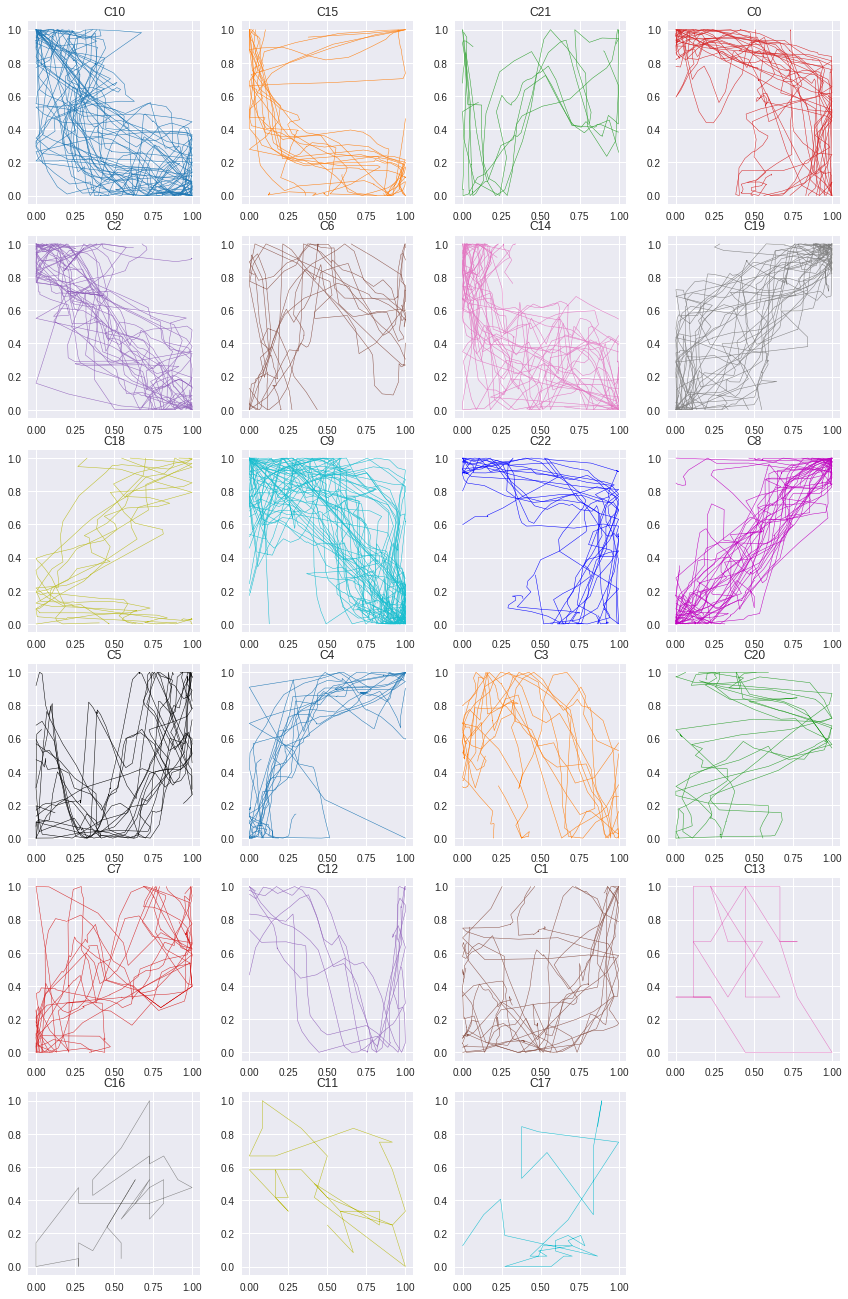
\includegraphics[width=\linewidth]{figs/clusters/CLU_H_ALL[MSM;c=.1].png}
    \caption{MSM; Cost = 0.1}
  \end{subfigure}
  \hspace{.5em}
    \begin{subfigure}[c]{0.35\linewidth}
      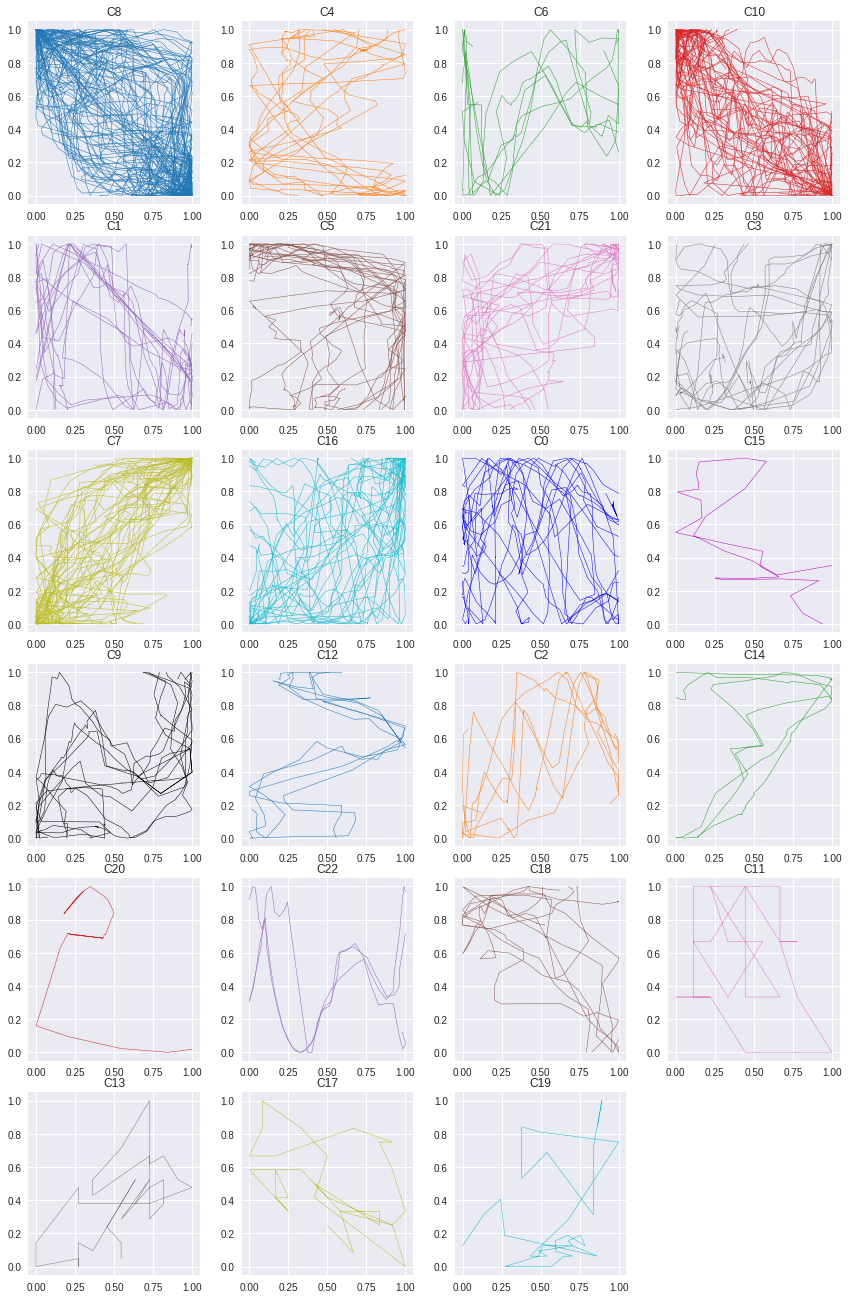
\includegraphics[width=\linewidth]{figs/clusters/CLU_H_ALL[MSM;c=.01].png}
    \caption{MSM; Cost = 0.01}
  \end{subfigure}
  
  \caption{Clusters generated by Move-Split-Merge with different parameter values.The top row is the affinity propagation Clusters and the bottom ones are from hierarchical clustering}
  \label{fig:cluster-msm}
\end{figure}


\begin{figure}[h]
  \centering
  \hspace{.5em}
   \begin{subfigure}[c]{0.35\linewidth}
     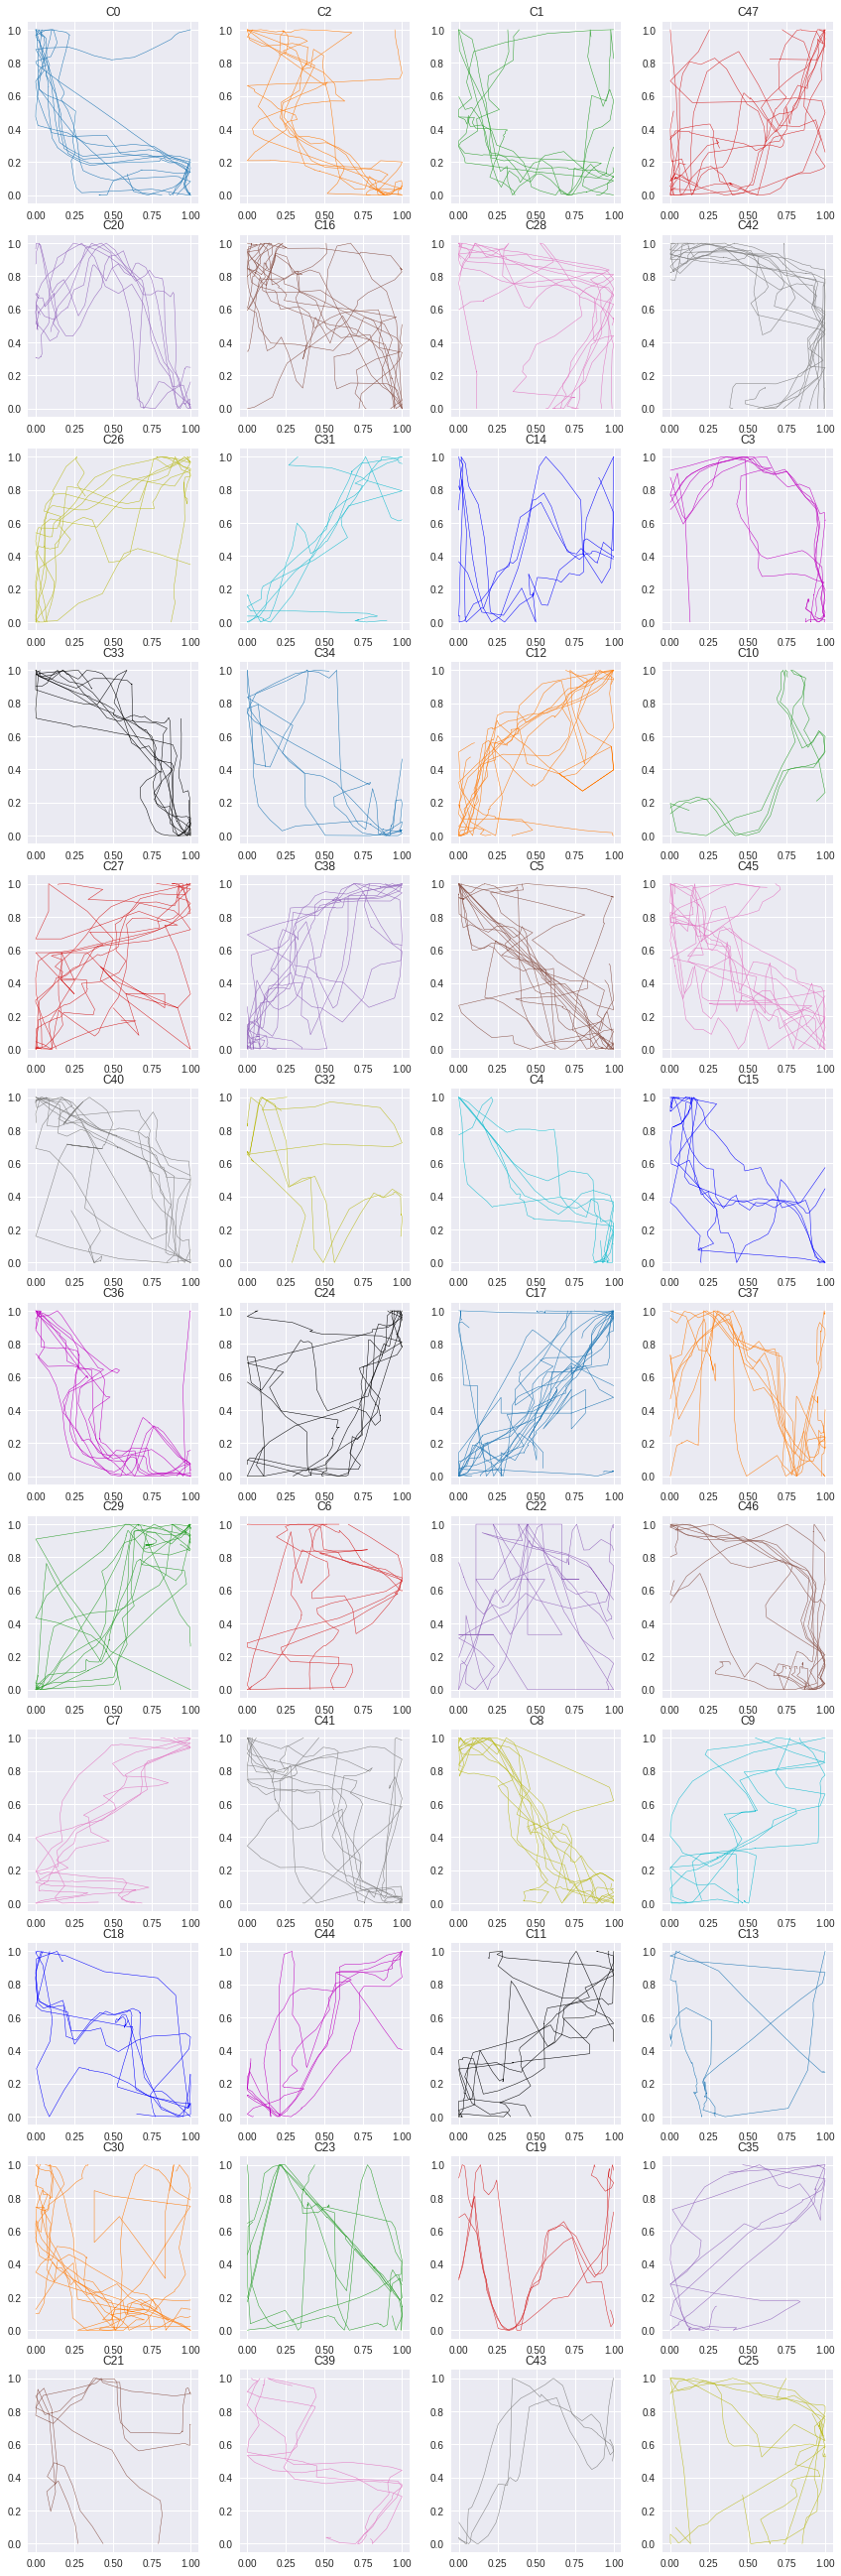
\includegraphics[width=\linewidth]{figs/clusters/CLU_AP_ALL[EDR;e=.101].png}
    \caption{EDR; $\epsilon=.101$}
  \end{subfigure}
  \hspace{.5em}
    \begin{subfigure}[c]{0.35\linewidth}
      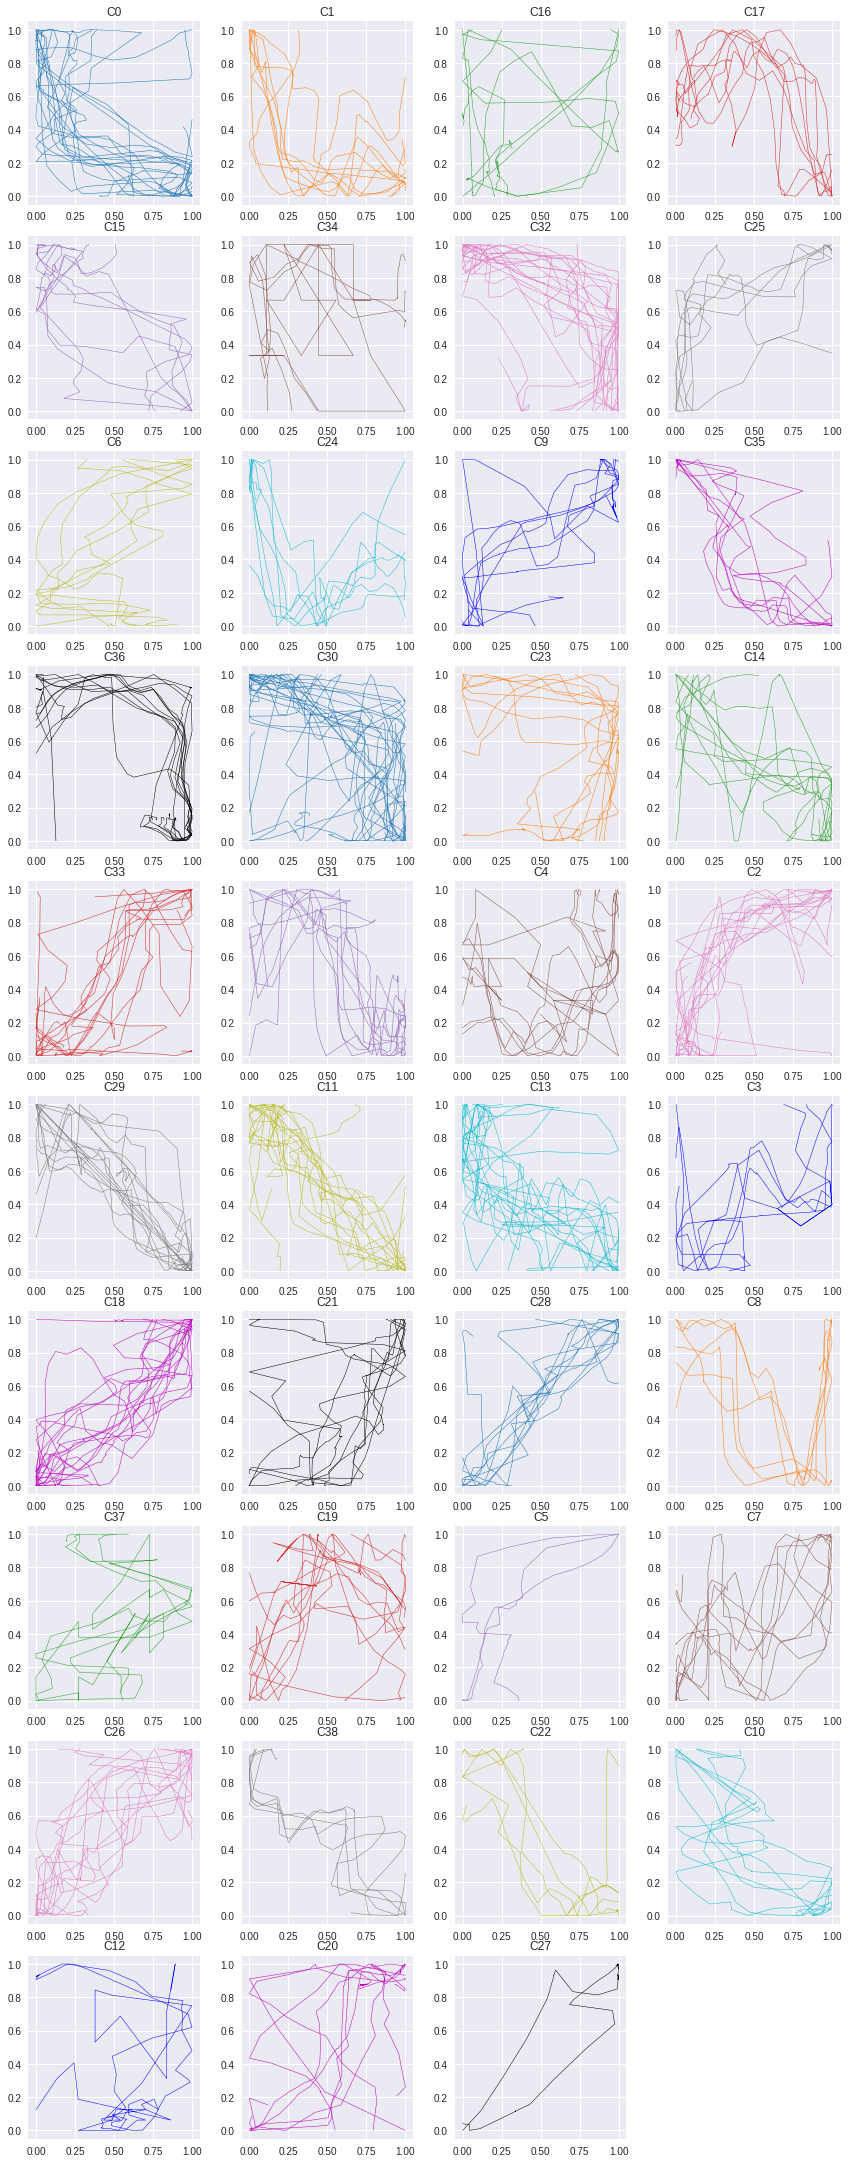
\includegraphics[width=\linewidth]{figs/clusters/CLU_AP_ALL[EDR;e=.203].png}
    \caption{EDR; $\epsilon=.203$}
  \end{subfigure}
  \hspace{.5em}
  
  \begin{subfigure}[c]{0.35\linewidth}
     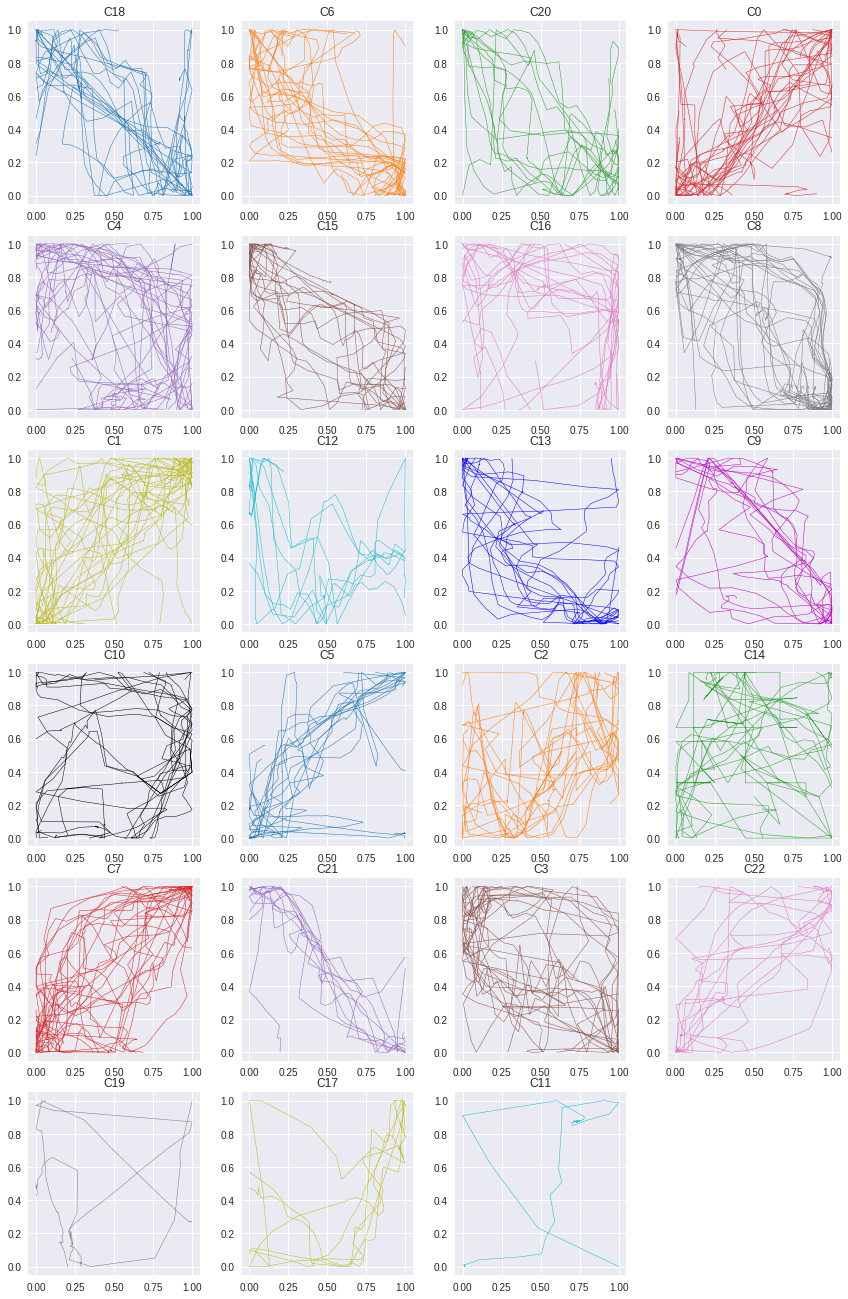
\includegraphics[width=\linewidth]{figs/clusters/CLU_H_ALL[EDR;e=.101].png}
    \caption{EDR; $\epsilon=.101$}
  \end{subfigure}
  \hspace{.5em}
    \begin{subfigure}[c]{0.35\linewidth}
      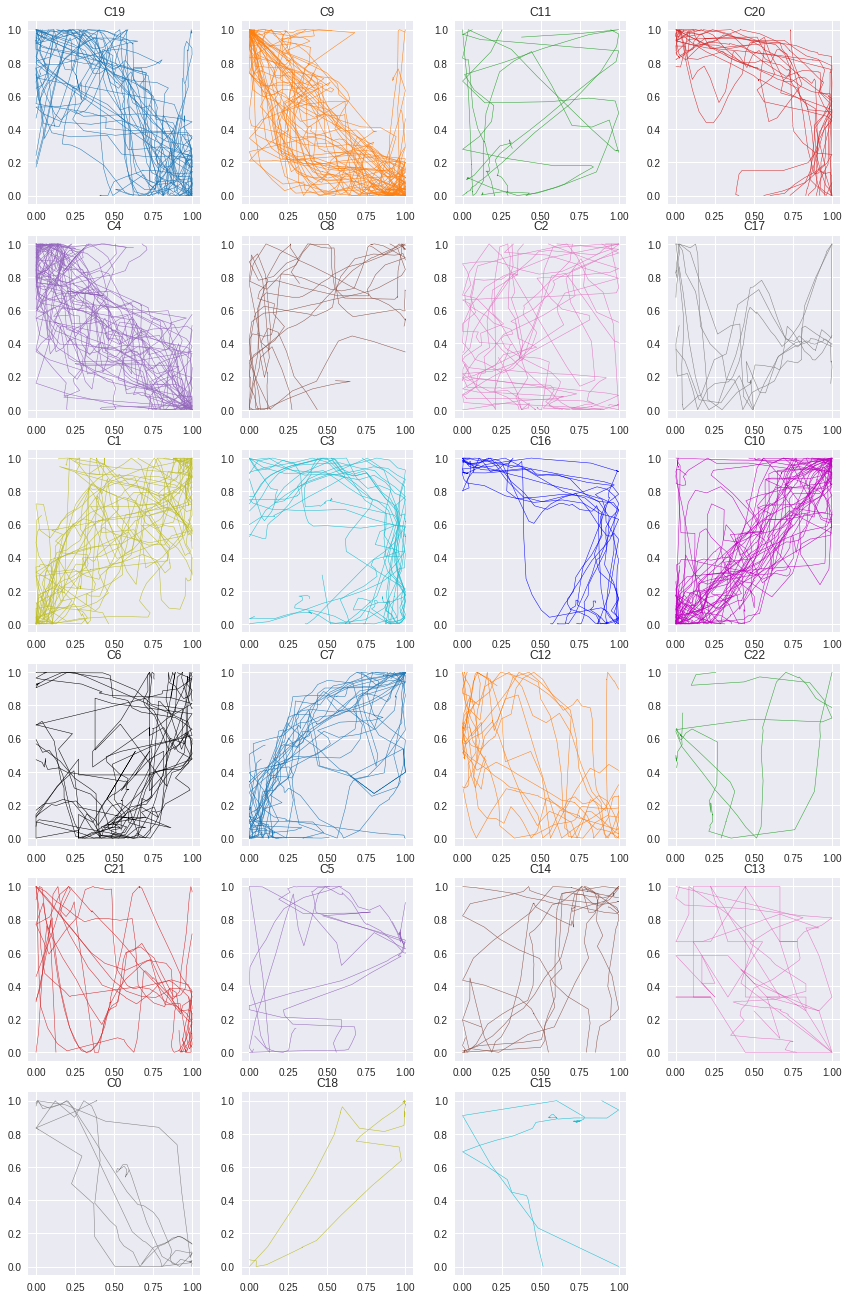
\includegraphics[width=\linewidth]{figs/clusters/CLU_H_ALL[EDR;e=.203].png}
    \caption{EDR; $\epsilon=.203$}
  \end{subfigure}
  \hspace{.5em}
 
  \caption{Clusters generated by Edit Distance on Real Sequence with different parameter values.The top row is the affinity propagation clusters and the bottom ones are from hierarchical clustering}
  \label{fig:cluster-edr}
\end{figure}



\begin{figure}[h]
  \centering
  \begin{subfigure}[c]{0.3\linewidth}
    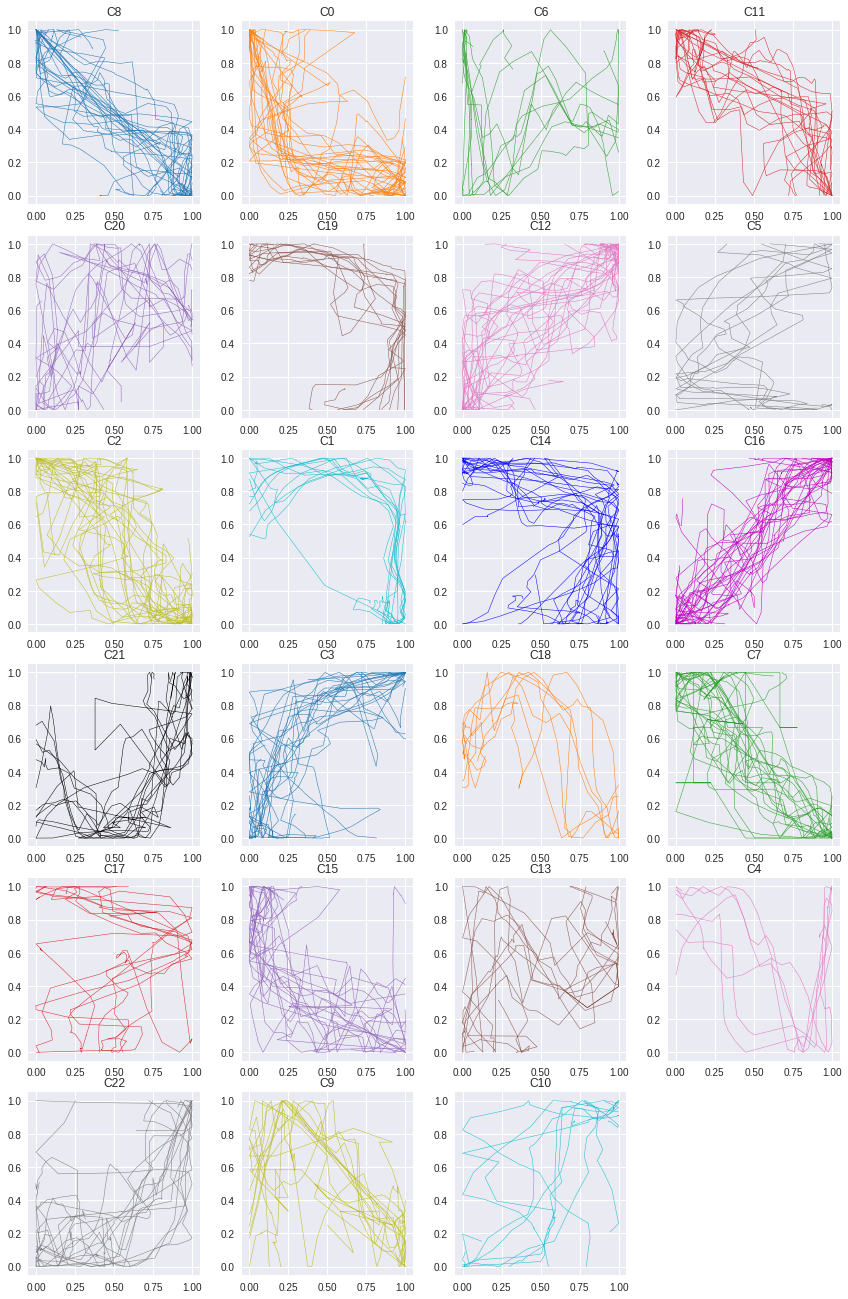
\includegraphics[width=\linewidth]{figs/clusters/CLU_AP_ALL[DTW].png}
    \caption{DTW}
  \end{subfigure}
  \hspace{.5em}
   \begin{subfigure}[c]{0.3\linewidth}
     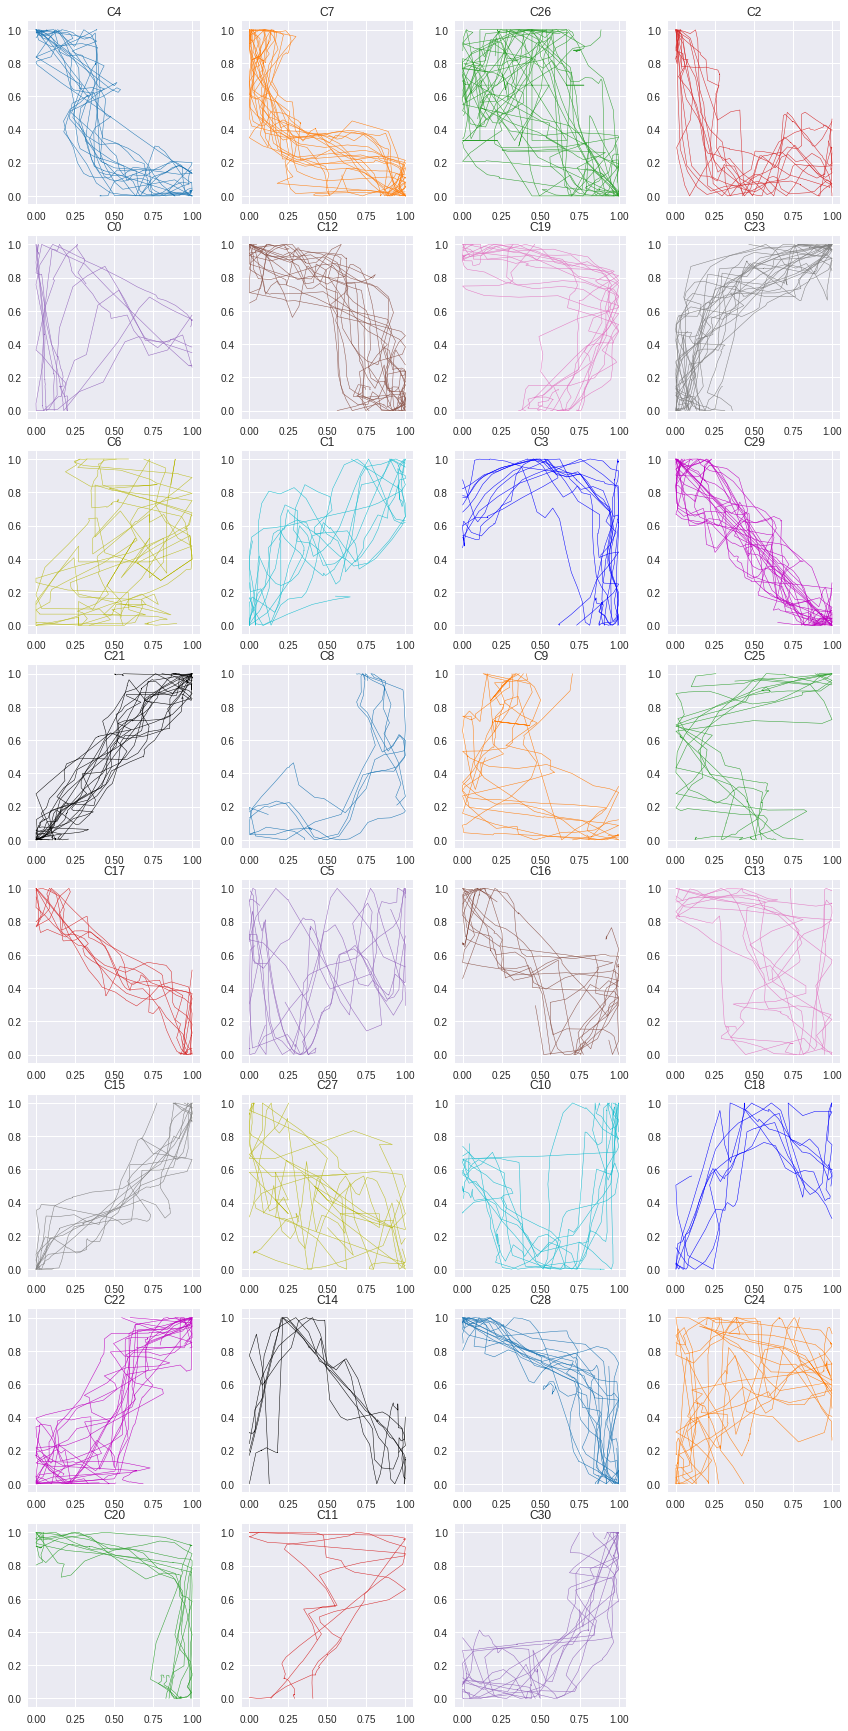
\includegraphics[width=\linewidth]{figs/clusters/CLU_AP_ALL[Hd].png}
    \caption{Hausdorff}
  \end{subfigure}
  \hspace{.5em}
    \begin{subfigure}[c]{0.3\linewidth}
     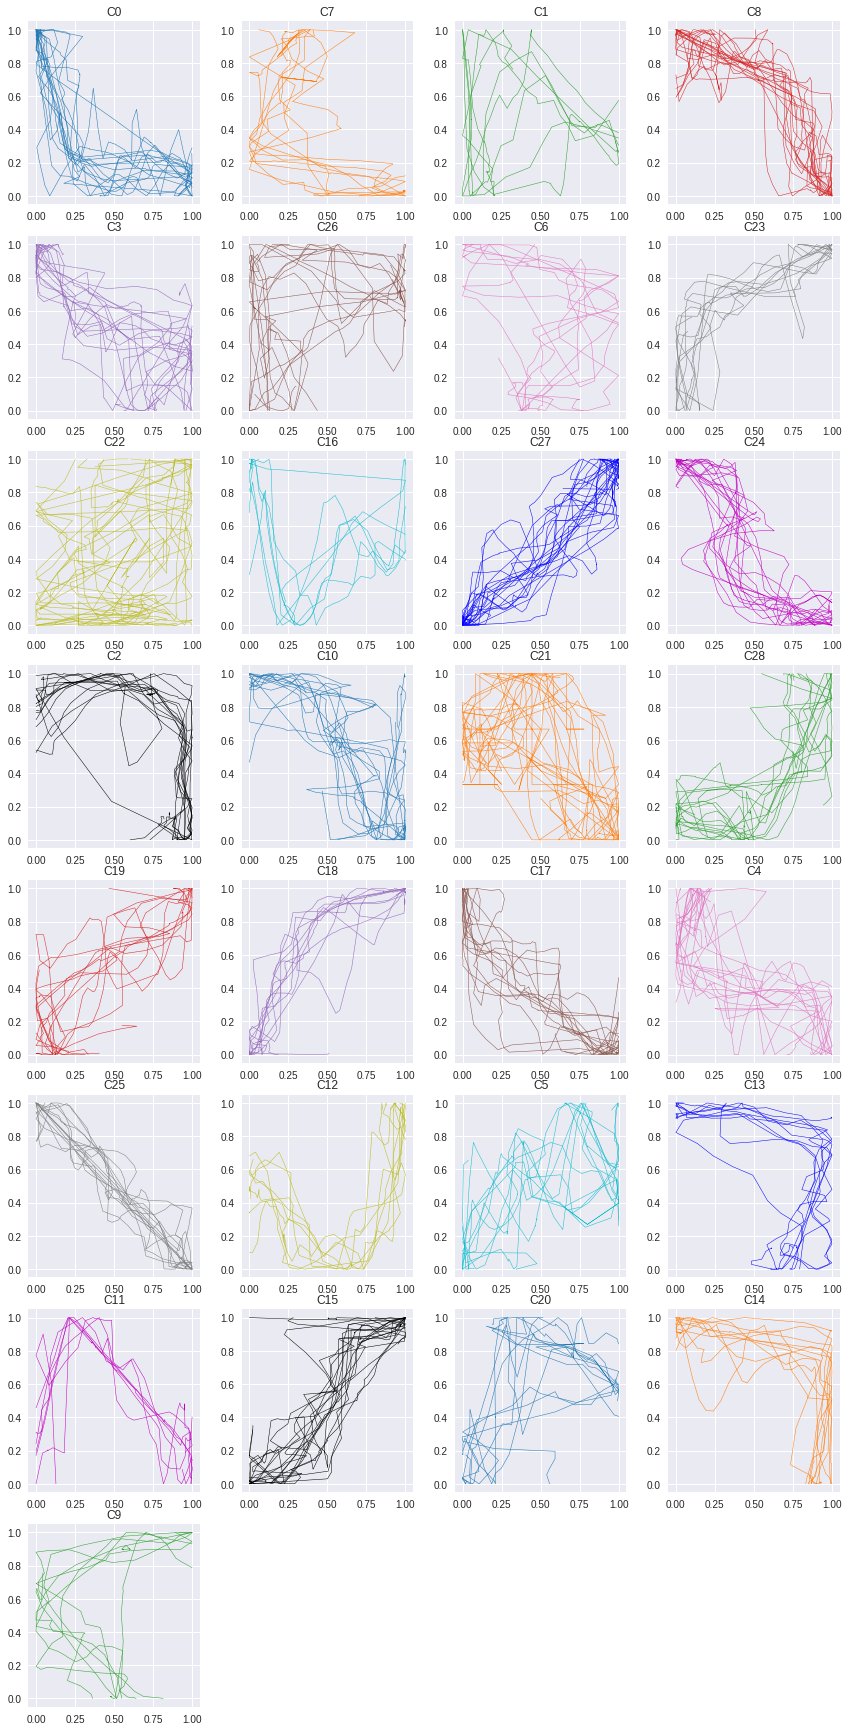
\includegraphics[width=\linewidth]{figs/clusters/CLU_AP_ALL[SSPD].png}
    \caption{SSPD}
  \end{subfigure}
  \hspace{.5em}
  \begin{subfigure}[c]{0.3\linewidth}
    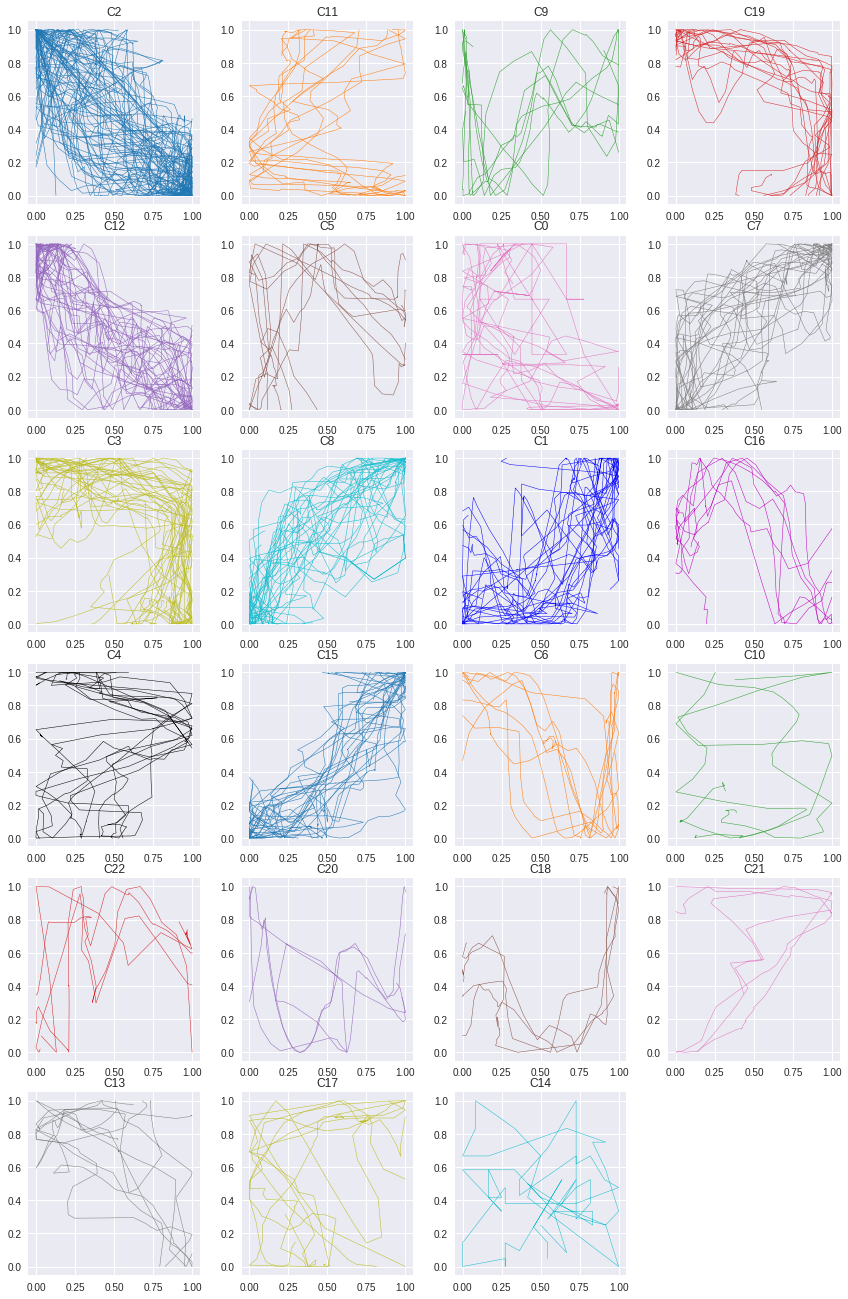
\includegraphics[width=\linewidth]{figs/clusters/CLU_H_ALL[DTW].png}
    \caption{DTW}
  \end{subfigure}
  \hspace{.5em}
   \begin{subfigure}[c]{0.3\linewidth}
     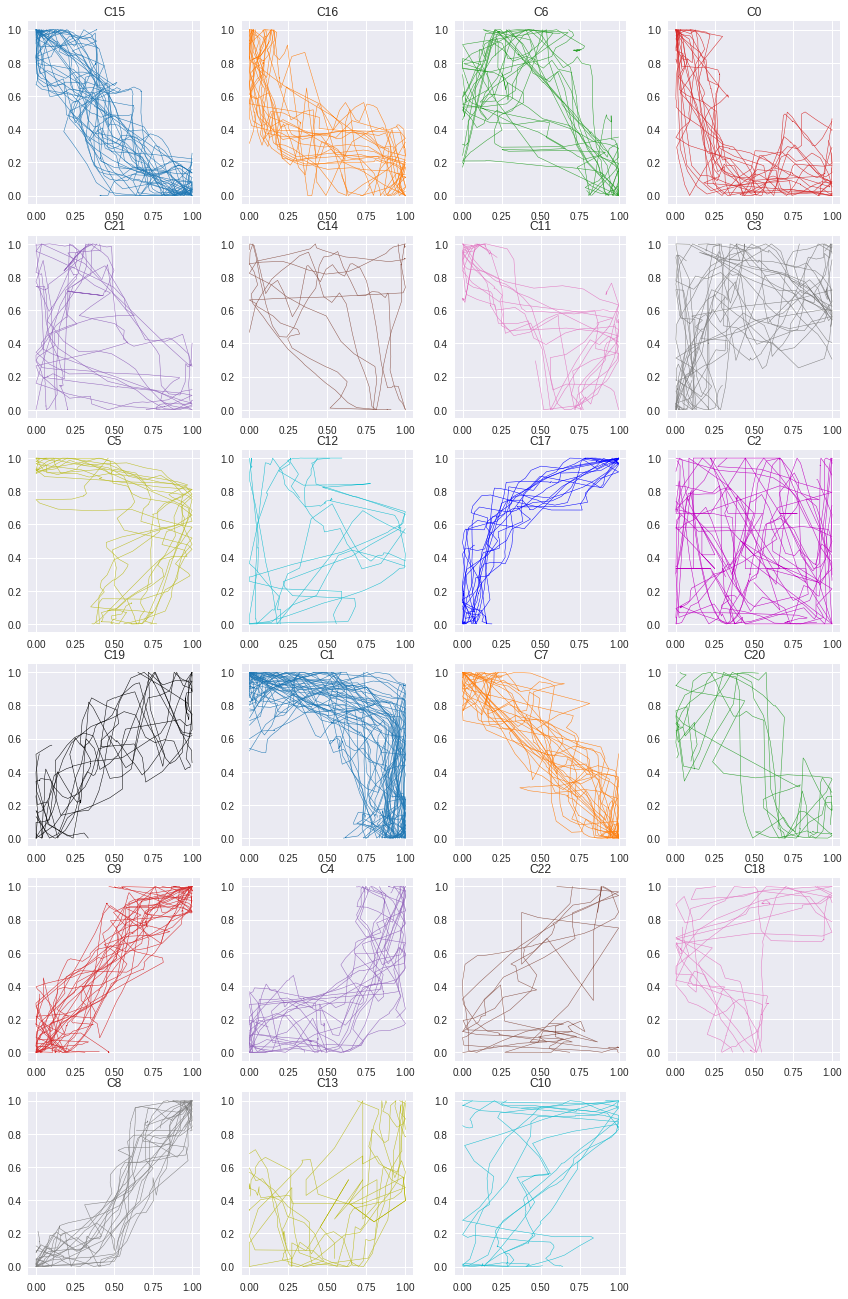
\includegraphics[width=\linewidth]{figs/clusters/CLU_H_ALL[Hd].png}
    \caption{Hausdorff}
  \end{subfigure}
  \hspace{.5em}
    \begin{subfigure}[c]{0.3\linewidth}
     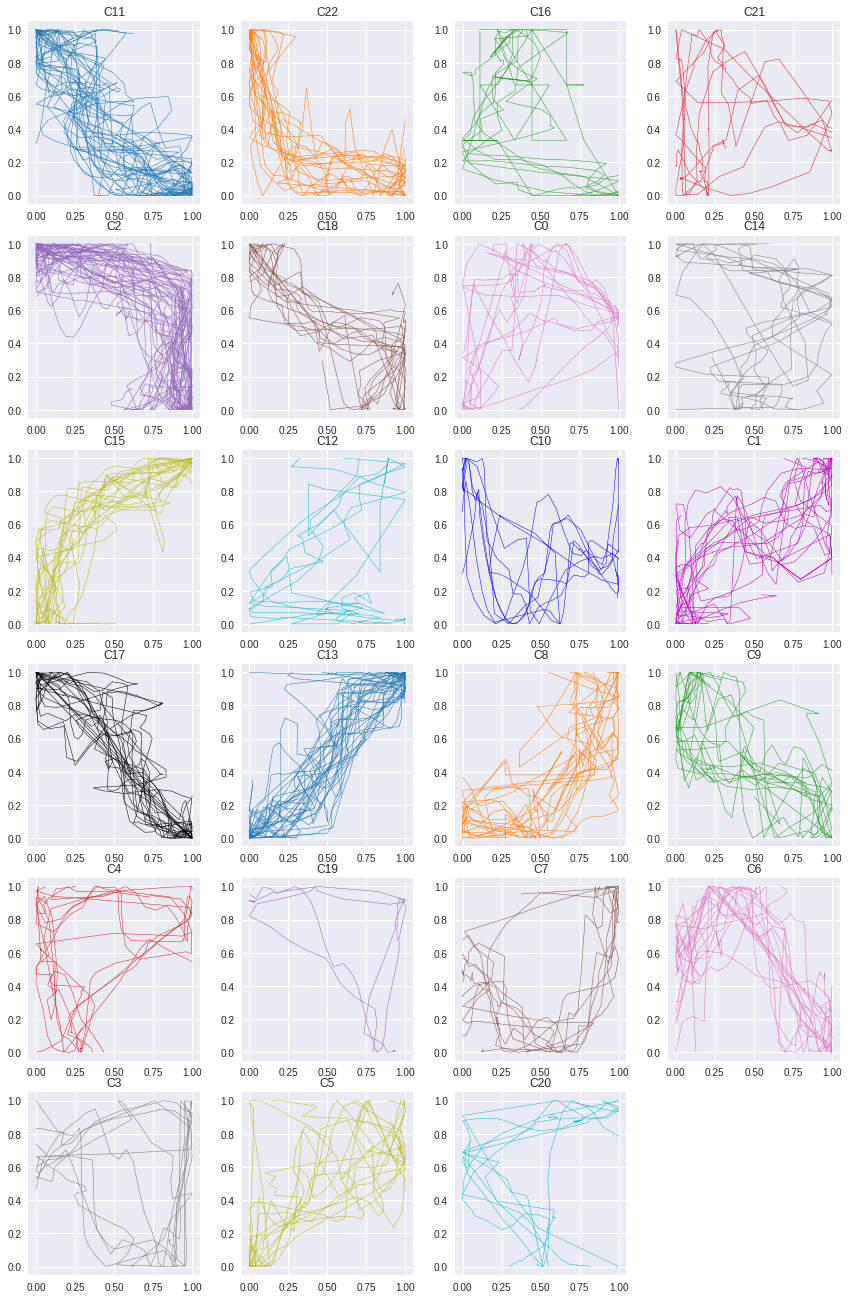
\includegraphics[width=\linewidth]{figs/clusters/CLU_H_ALL[SSPD].png}
    \caption{SSPD}
  \end{subfigure}
  \caption{Clusters created with DTW, Hausdorff and SSPD. The top row is the affinity propagation clusters and the bottom ones are from hierarchical clustering}
  \label{fig:cluster-dtw-hd-sspd}
\end{figure}




% TABLE X contains the Davies-Bouldin results of each for each cluster per type of clustering method.
% We note that SSPD and HD have resulted in the least clear clusterings using both the agglomerative hierarchical method and affinity propagation. 

% As elaborated upon in CHAPTER, human discretion remains one of the key ways to evaluate clustering task results [79]. Figures [A-Z]  are the graphical representations of the clustering results of the two best and two worst measures for each clustering technique. 


% \begin{figure}[h]
%   \centering
%   \begin{subfigure}[c]{0.35\linewidth}
%     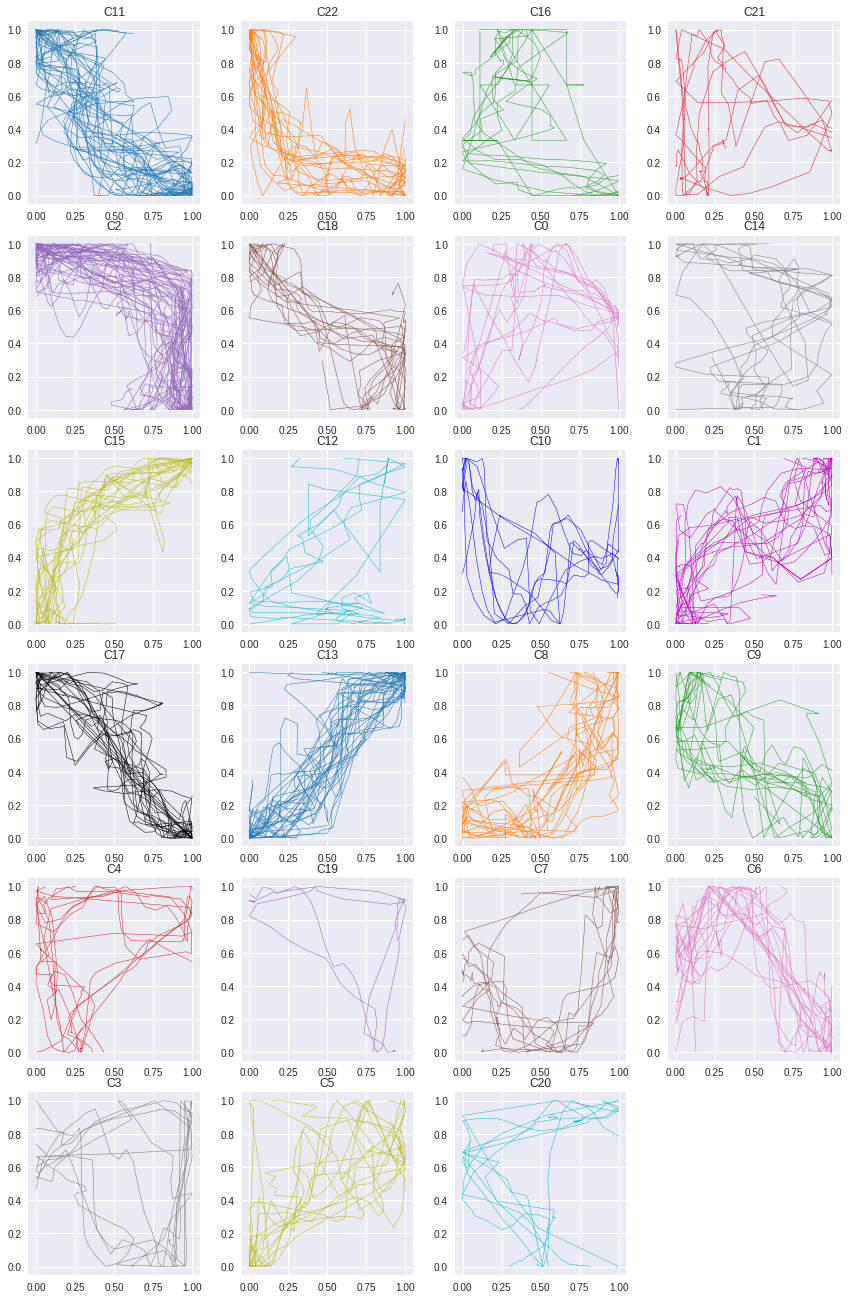
\includegraphics[width=\linewidth]{figs/clusters/CLU_H_ALL[SSPD].png}
%     \caption{Symmetric Segment Path Distance}
%   \end{subfigure}
%   \hspace{1em}
%   \begin{subfigure}[c]{0.35\linewidth}
%      \includegraphics[width=\linewidth]{figs/clusters/CLU_H_ALL[HD].png}
%     \caption{Hausdorff Distance }
%   \end{subfigure}
%   \caption{Final HCA-Clusters of the measures the worst Davies-Bouldin Index}
%   \label{fig:cluster-h-worst}
% \end{figure}

% For the sake of brevity, only a handful of the clustering are shown in detail and the remaining graphical representations are found in the APPENDIX. 
% Figures [A-Z] are the graphical representations of the clustering results of the two best and two worst measures for each clustering technique. 

\chapter{Discussion}
\label{ch:7}
In this chapter, we seek to contextualize the results from the preceding chapter. 
We apply theory from \Cref{ch:2} and compare the result to the expected behavior 
% expect from what we know about their theoretical construction/base. 

\section{Similarity Scores}

We have established that the measures define what makes trajectories similar. 
Some of the measures have a similar base idea, and thus we expect to see this reflected in the results. 
From the rankings of most similar pairs, there are a few things that stand out and we will go over them here.


%We reiterate this is not the case for all of them, and consequently, not all columns of TABLE can be used in this manner. 

First of all, EDR with $\epsilon$ set to 0.203 was the column in \Cref{tab:top-10-sim-pairs} which had the least number of frequent “most similar pairs”. 
When adjusting the parameter down to 0.101, our approximation of the recommend parameter value, all of its eight most pairs were found elsewhere in the table.
Recall that EDR’s parameter is the threshold distance that determines if points are “matching”. 
The similarity ranking with the lower parameter value aligns more with the other measures, and this could indicate that the other threshold was set too high.
We would presume that EDR would give a similar ranking as the other noise-tolerant edit-distance inspired method, MSM.
From what can be seen in the table, this appears to hold, but it varies with its parameter value too. 

%   that would have similar values to the

Next, we note that the Hausdorff distance generated similar pairs which were quite different from the other measures. 
As the Hausdorff metric is parameter-free, we reckon that the reason its results stood out was that it defined trajectory similarity in a different manner than the rest. 
We established that the Hausdorff distance does not take into account the direction of a trajectory and the only other measure that is invariant to direction is SSPD. 
Indeed they share many of the top 10 ranked scores, however, SSPD distinguishes itself Hd as it reduces the similarity score to a single element-element pair making altering their internal rankings again. 

% Next we observe that the Hausdorff distance contains the second least “frequent pairs” and as it parameter free, we reason that there must be something with how it defines trajectory similarity that makes it stand out. Recall that the Hausdorff distance stood out as the only measure that did not take into account the direction of a trajectory. Furthermore, it stands out as the only measure that reduces the similarity distance to an element-element pair.

The final observation from \Cref{tab:top-10-sim-pairs} we noted was that Euclidean distance, ERP, and one of the MSM measures gave the exact same top 10 pairs. 
Upon closer examination, it turned out that their ranking remained the same until the 44th pair, and the similitude between the measures continued beyond that.
MSM with cost value 1 and the Euclidean distance's ranking match for 9456 of the 10 thousand most similar trajectory pairs. 
We reason that this occurred as a consequence of the cost of Splits and Merges being set too high, making MSM  default to the Move operation whose cost is the $L_2$ norm between trajectory elements.
As for ERP, we reason that setting the reference point, $g$, to the origin, increased the cost for trajectory elements that were far away.
Again, making the method depend on the $L_2$ norm between trajectory elements as the cost of an edit.


\section{Davies-Bouldin Results}

The essence of this thesis is to examine how the definition of similarity varies with different measures.
Clustering is a manner of grouping the trajectories such that traits which are seen as the most defining characteristics under various definitions get highlighted. 

As stated in \Cref{ch:2}, there are a number of cluster evaluation techniques that aim to numerically rank the quality of clustering results.
One of these is the DB-index however we will not an assumption regarding which type of type similarity was the most “correct” one.
The ranking created by this criterion is not invalid, but the insight it adds to is limited.
Nevertheless, we have chosen to leave in this stage of the experiment and in the report on the account of the efforts that were put into computing it as well as its natural role as a starting point for analyzing the clusters. 
 
Our version of Davis-Bouldin favors clusterings where each trajectory element differs as little as possible from the mean of all trajectory elements when computed in a. A consequence of this is that the cluster can appear fuzzy since the placement of the surrounding points does not affect the index. 
From \Cref{tab:cluster-dbidx} it appears as if the lock-step method and EDR with threshold parameter $\epsilon=0.203$ were the best performing methods, and this is as expected. 

Moreover, methods that do not take into account order observations, or methods that would reorder the trajectory elements received low DB-index rankings. In \Cref{fig:cluster-best-worst-db-ap,fig:cluster-best-worst-db-h}  the clusters that were generated by the measures which received highest and lowest DB-indexes are drawn. These figures illustrate the bias of our DB-index implementation. 


\begin{figure}[h!]
  \centering
  \hspace{1em}
   \begin{subfigure}[c]{0.37\linewidth}
     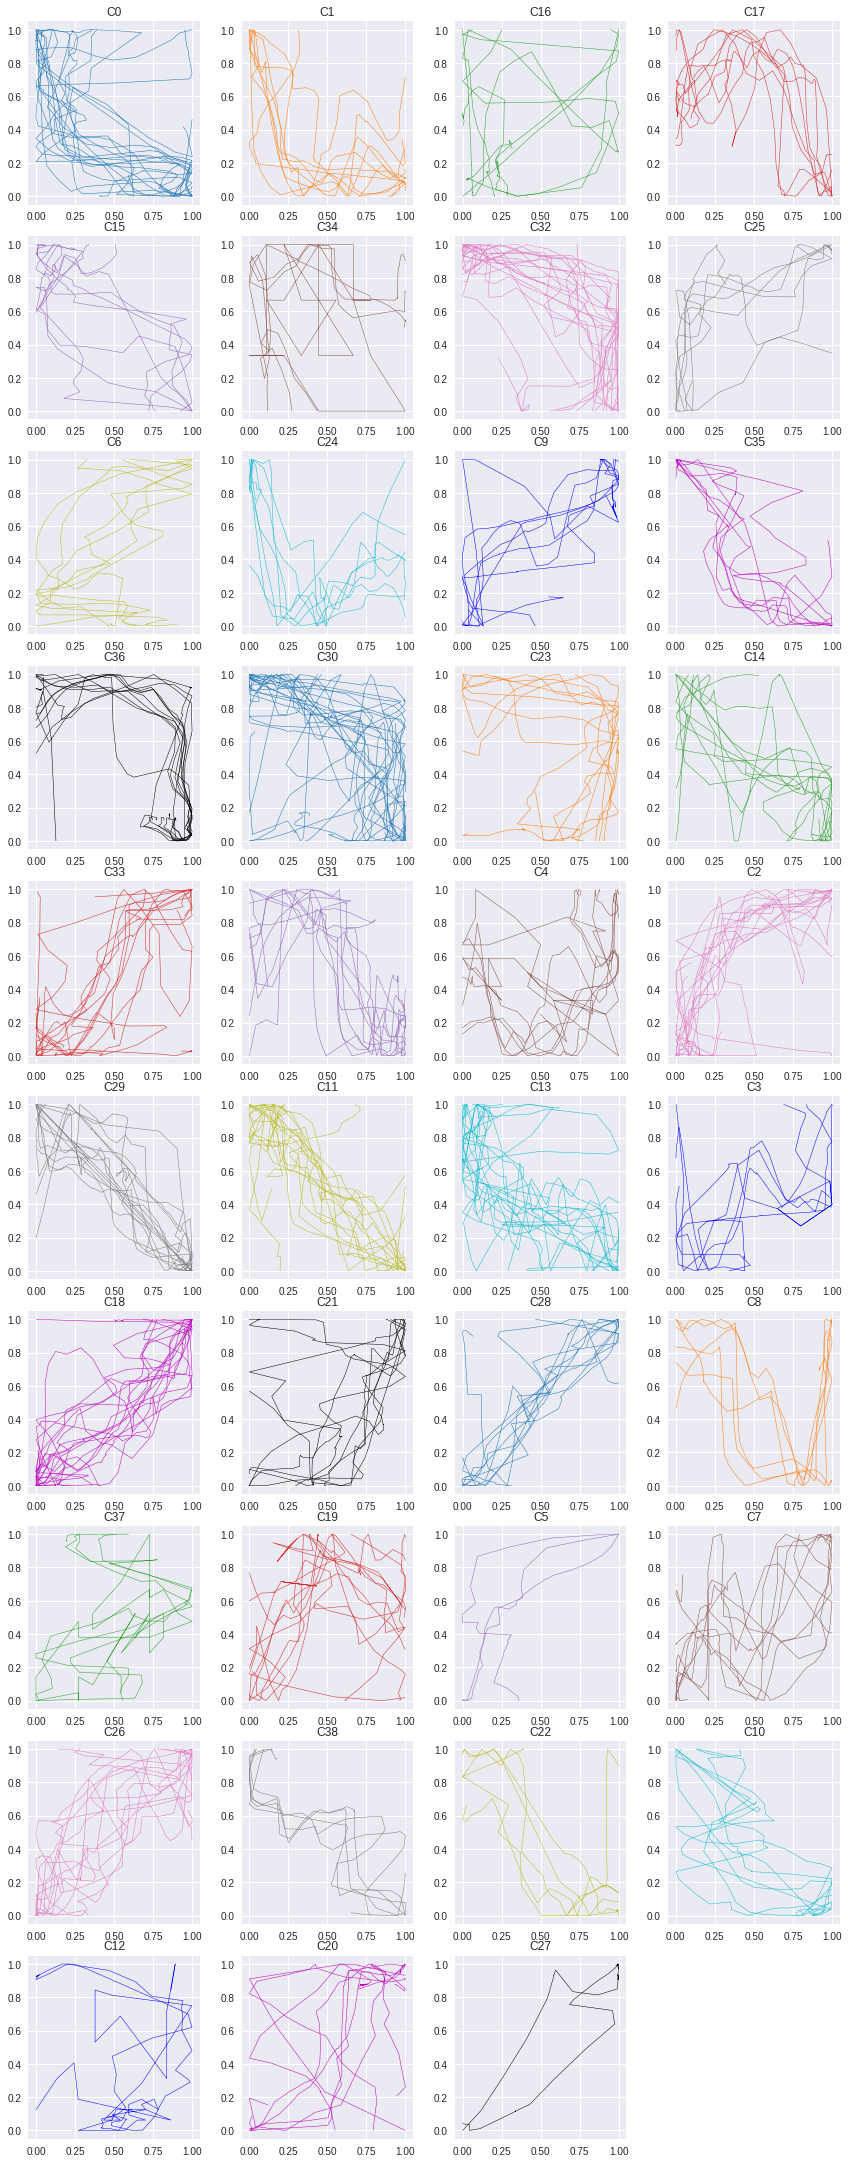
\includegraphics[width=\linewidth]{figs/clusters/CLU_AP_ALL[EDR;e=.203].png}
    \caption{EDR;$\epsilon=0.203$, highest rank}
  \end{subfigure}
  \hfill
  \begin{subfigure}[c]{0.37\linewidth}
    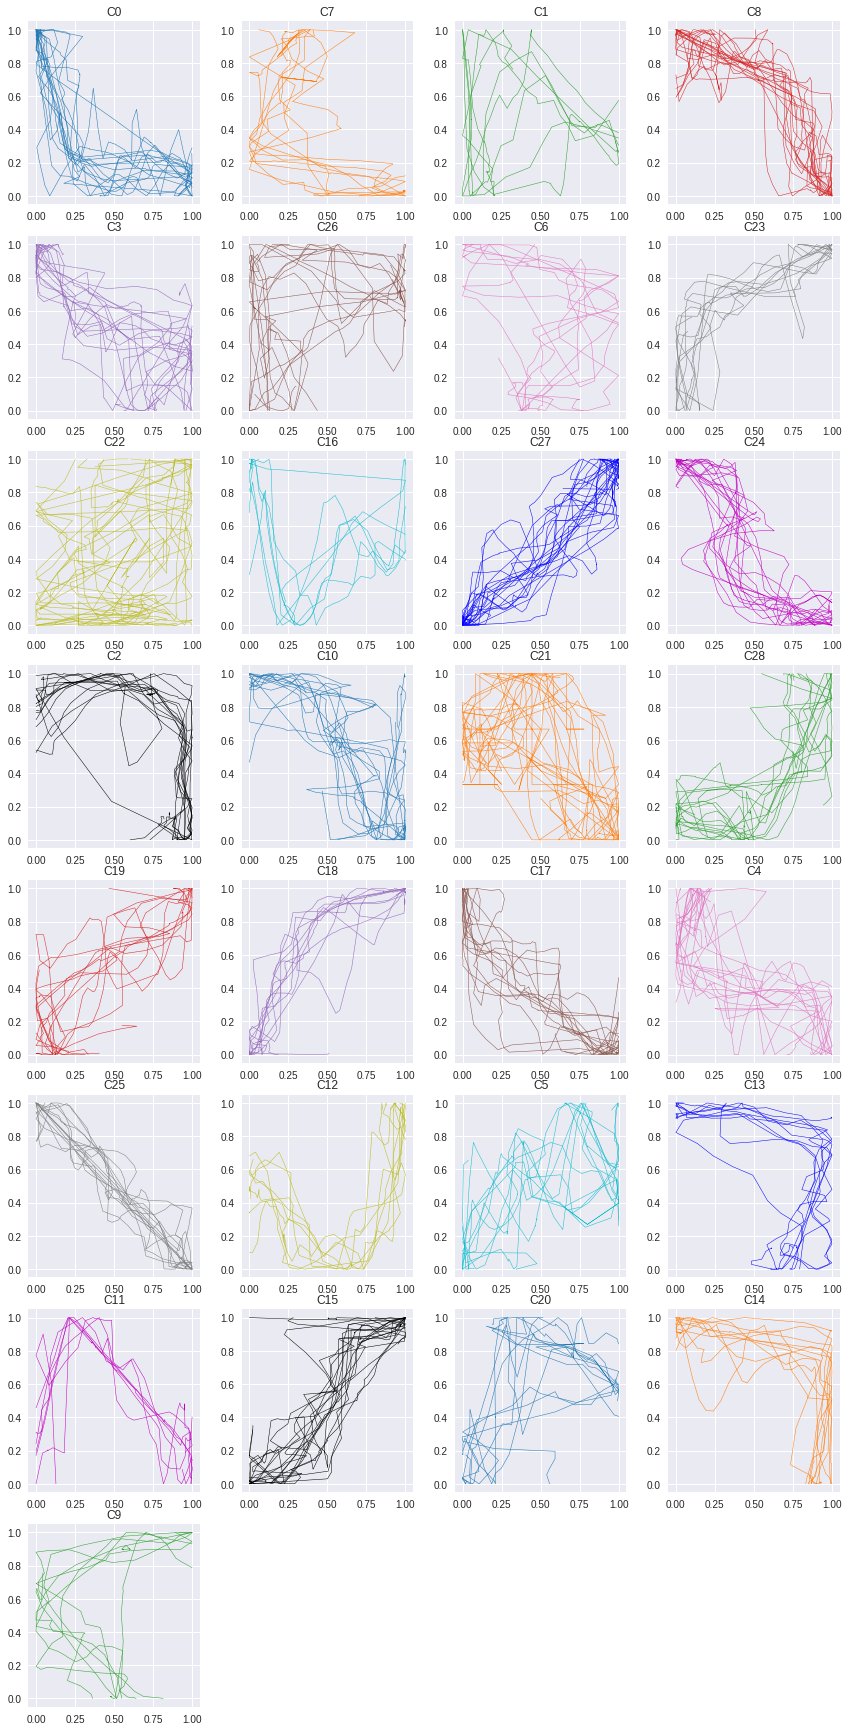
\includegraphics[width=\linewidth]{figs/clusters/CLU_AP_ALL[SSPD].png}
    \caption{SSPD, lowest rank}
  \end{subfigure}
  \caption{The AP-clusters of the measures the best and wort Davies-Bouldin indexes.}
  \label{fig:cluster-best-worst-db-ap}
\end{figure}

\begin{figure}[h!]
  \centering
  \hspace{1em}
   \begin{subfigure}[c]{0.4\linewidth}
     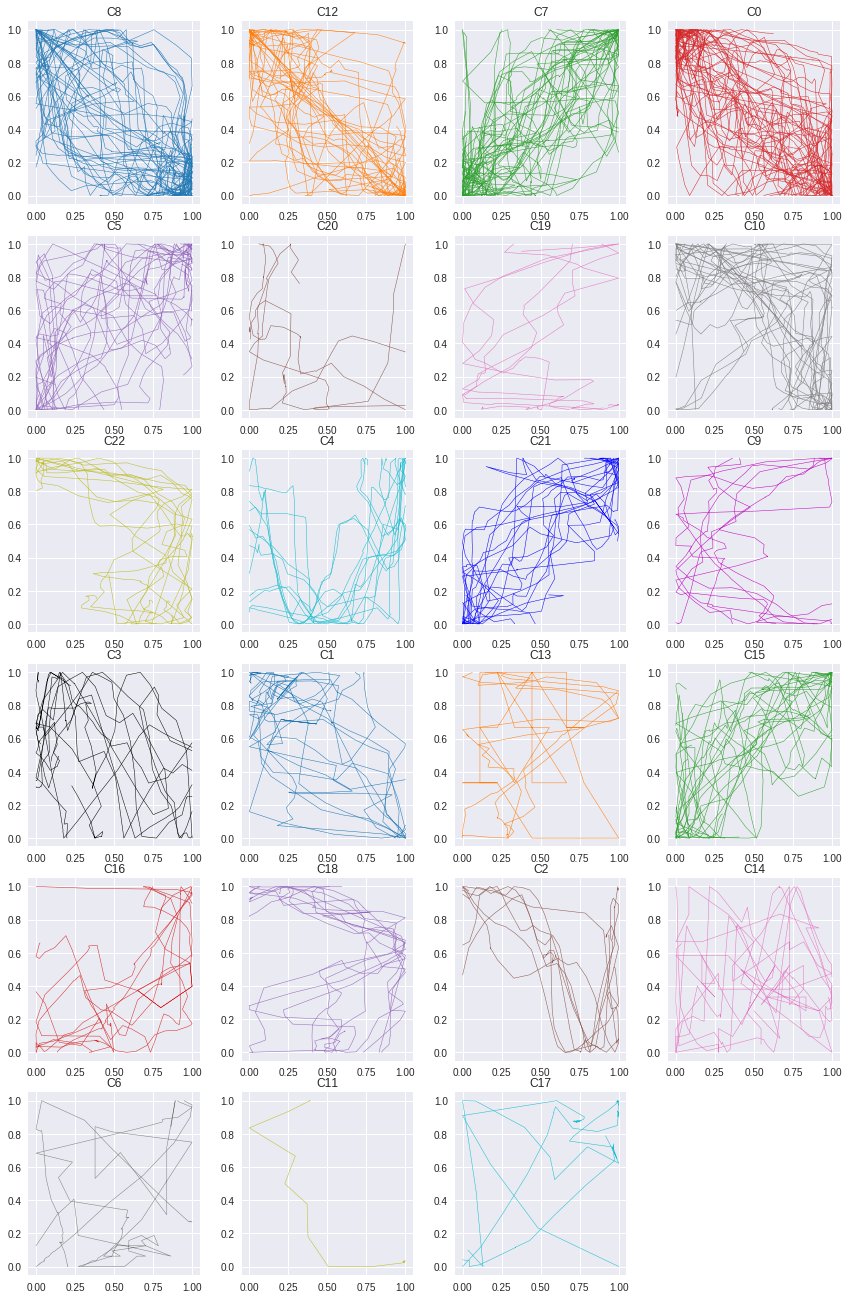
\includegraphics[width=\linewidth]{figs/clusters/CLU_H_ALL[ERP;g=0,0].png}
    \caption{ERP, $\epsilon=0.203$, highest rank}
  \end{subfigure}
  \hfill
  \begin{subfigure}[c]{0.4\linewidth}
    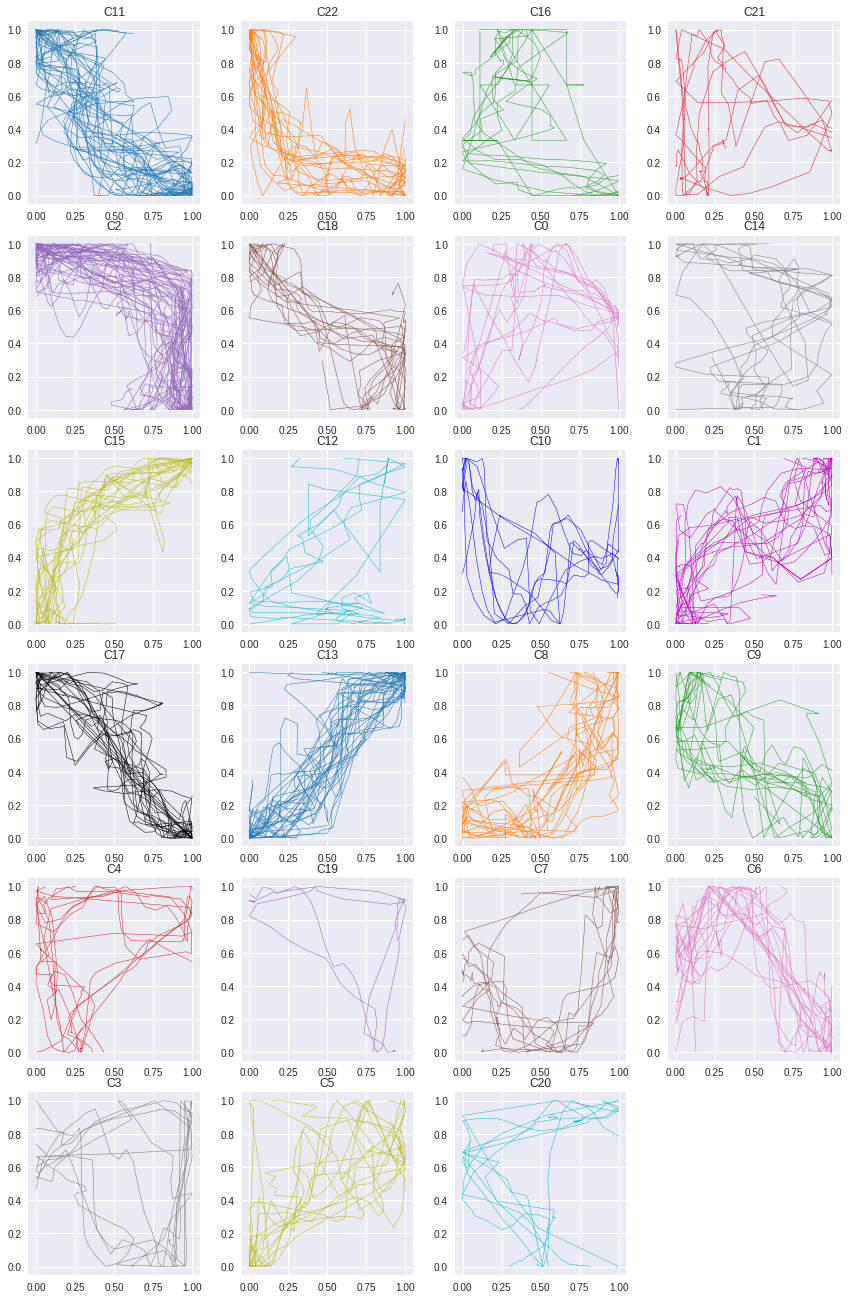
\includegraphics[width=\linewidth]{figs/clusters/CLU_H_ALL[SSPD].png}
    \caption{SSPD, lowest rank}
  \end{subfigure}
  \caption{The HCA-clusters of the measures the best and wort Davies-Bouldin indexes.}
  \label{fig:cluster-best-worst-db-h}
\end{figure}



As a consequence of the unreliability of the DB-index, the main tool for examining the clusters will be visual inspection.
This will allow us to account for the different aspects of trajectory similarity and formulate conclusions accordingly. 
Re-examining \Cref{fig:cluster-best-worst-db-ap,fig:cluster-best-worst-db-h} with visual inspection it would appear that SSPD produced cleaner and fewer clusters than both EDR and ERP. 
This is in stark contrast to the ranking created by the Davies-Bouldin criteria under both HCA and AP analysis. 


This evaluation alternative comes with its own drawbacks, one of which is the matter of subjectivity. 
At the same time, it has been stated that human assessment is an important component for determining the quality of clusters\cite{79-SilhouetteAnalysis}. 
We will not be declaring any measure better than the others as our results do not provide support for an accurate ranking.



% We cannot declare one measure just better than all others from the evaluation that we executed here as it makes no sense. This is in large part due to the inherent bias of using a strict lockstep method to evaluate the final clusters. 
% By visual inspection, SSPD produced cleaner and fewer clusters than EDR, $\epsilon=0.203$ under AP, despite having a much worse criterion. This pattern repeats itself under HCA when predetermined even with  the amount of final clusters. EDR  as well \Cref{fig:cluster-best-worst-h-db}.

% Based on those arguments, the main tool for examining the clusters will be visual inspection. This will allow us to account for the different definitions/aspects of similarity and formulate conclusions in an aggregate manner. 
% This method comes with its own drawbacks, one of which is the matter of subjectivity. Yet as brought up in supported previous works[CITATIONS], human assessment key for determining the quality of clusters. 




\section{Cluster Behavior}

First, we describe what we expected the clusters to look like based on the properties of the specific similarly distance function. 
For the methods that operate with a parameter value, we discuss how changing that value would affect the cluster results.
Then we compare our expectations to the clusters themselves.
Affinity propagation is a was the parameter-free method, thus its results are weighted more.
On the other hand, the number of hierarchical clusters was arbitrarily set, leading us to use its results as a supplementary evaluation. 


% https://www.wordhippo.com/what-is/another-word-for/foreseeable.html 
\subsection{Expectations}
In general, there are three factors that will affect how we expect the final clusters to appear. 
Measures that are context-aware should calculate fewer fuzzy clusters.  
Next, measures that account for local time shifts should group trajectories that have similar sub-sections but with an offset creating a wider band of similarity.
Lastly, we expect the noise-sensitive trajectories to create fuzzier trajectories.  


\textbf{Euclidean Distance} is the only lock-step measure, and trajectories that are in the same region might receive an artificially high similarly score by nature of being near each other. 
A trajectory pair will be rewarded if they have elements at the same index which are near each.
This would create fuzzy clusters as each point evaluated isolation and taking the average of the pairwise element-distances will artificially smooth out the distances.
An extra amount of fuzziness is expected to come from the fact that this measure is sensitive to noise. 

% WE COULD observe that there are trajectories that oscillate around the same region at a similar pace- giving them a lock-step similar score, but the cluster ends up looking fuzzy. 

\clearpage
\textbf{Dynamic Time Warping}  optimizes for local shape similarity and warps trajectories to reflect similarity after shape-preserving transformations.
We expect the final clusters to appear fuzzy at first glance as the local similarities would be out of sync. 
Yet upon closer examination, we should be able to spot bands of cohesive trajectory sections. 
DTW is a noise-sensitive method, so we would expect some level of fuzziness to be present, however, the clusters should be crisper than that of the Ed. 



From \textbf{Hausdorff Distance}, we would expect crisper clusters than both Ed and DTW if we could guarantee the data free of noise.
The maximizing over a minimum of all element-element pairings means that the overall shape similarity is weighted in a way that the other measures do not account for. 
In other words, the global resemblance matters more under this definition. 
However, the data set we used is not noise-free so while we expect some crispness, there will be fuzziness of the clusters due to its noise sensitivity.

% All of the trajectories' points have to be near each other for if the pair is to receive a high similarity score.
% stemming from the reduction of similarity distance to distance between two trajectory elements. 

One of the key features of \textbf{Symmetrized Segment-Path Distance} is that it accounts for whole trajectory shape similarity. 
This means that we expect it to generate the crispest looking clusters. 
The expectation of crisp clusters is further substantiated by its tolerance to noise
This method aimed to be invariant to the physical locations, meaning that trajectories of similar shapes with different origins could be grouped together. This could result in some broader bands of similarity.

% All of the parametric measures adapt to local time shifts like in the same manner as DTW, and  therefore we expect the clusters they generate exhibit some of the same type of fuzziness. This, of course, is not the only factor that affects how fuzzy or crisp the clusters become. The choice of parameter, as well as the (internal workings) of the algorithms matter greatly.  
%SOMETHING ABOUT HOW DTW ERP etc have re-s sim to dtw as noted in \cite{26}


Recall that \textbf{Edit Distance on Real Sequences} uses the parameter $\epsilon$ to as the matching threshold for how close how two trajectory elements are.
Decreasing the parameter value leads to an increase in strictness in how close elements have to be, and in turn, would lead to crisper clusters.
It goes without saying that a too restrictive $\epsilon$ would no longer be accurate; if no trajectory elements are matching, the only basis for similarity would be the trajectory lengths. 
Clusters are expected to have some level of fuzziness as EDR considers the trajectory element in isolation. 


\textbf{Edit Distance with Real Penalty} was computed with one parameter value.
We have established that this metric is sensitive to noise and that it accommodates local time shifts.
As EDR, this measure does isolates the trajectory elements when computing the similarity distance. 
This means that there are three factors that contribute to fuzzy clusters, thus we expect the fuzziest clusters to be generated from this metric.  
% As it is a measure that handles local time shifts and does not compare a trajectory as a whole, we expect the clusters to appear quite fuzzy. This expectation is further supported by its low tolerance to noise. 


\textbf{Move-Split-Merge} handles local time shifts in the same manner as DTW and the other Edit Distance-based measures.
We expect to observe trajectory sections that match and create wider bands. 
MSM distinguishes itself by accounting for the values that surround a given element when computing the similarity score. 
This means that we expect the clusters are crisper than those of generated by EDR and ERP. 
The parameter of MSM determines to which degree Splits and Merges are favored over Moves. 
As the cost increases, they will increasingly be evaded in favor of directly substituting the element. 
The cost of a Move is pairwise element-element distance, and in turn, the clusters would resemble those created by a Euclidean distance based measure. 
On the other hand, if the parameter is set too low we expect more trajectories that do not resemble each other to get clustered together. 


%I thin,, it is hard to tell

% Finally we study how we expect the change of the cost of MSM transformations to impact the final clusters. The parameter determines how much splits and merges should be favored over moves. At the extreme end, MSM will resemble DTW as element-element distance would dominate the cost matrix. That is, the higher the value of c, the more the cluster should resemble DTW. For lower values of c, we should see a preference for actively splitting and merging, bringing its cluster results closer to that of ERP. 

% Setting the cost to 1, results in similarity scores that are


\subsection{Visual Inspection}

The visual inspection inspects the apparent fuzziness of the clusters as well as how scatted the trajectories within a cluster are. 
We will refer to the latter of these characteristics as the \textit{band} of similarity which describes the general \textit{trend} of the cluster. 
Where is it possible, we remark how larger trajectory sections were processed. 
Unfortunately, spotting tendencies like that is not something visual inspection excels at.

In the case of affinity propagation, we take note of how many clusters it generated. 
The corresponding evaluation for the hierarchical clusters is taking note of how balanced the final clusters are.
With how hierarchical clusters are created, some imbalance is expected as the most distinct trajectories will be connected last.

% contour  
%  silhouette
%  hierarchical affinity

\textbf{Euclidean Distance:}
\begin{itemize}
\item AP:  In terms of overall shape, the clusters appear very fuzzy. 
There are some clusters where that have a clearer contour and some where it is possible to spot a trend for the trajectories. 
Nevertheless the general impression remains fuzzy; we observe trajectories that seem to oscillate freely around the apparent trajectory band.
While oscillations make the clusters appear fuzzier, the clusters do not come across as randomly grouped observations. 

\medskip
\item HCA: There appears to be a bias and clusters are unbalanced. 
Some of the clusters contained a few trajectories while some of them encompassed a large number of them.
In those clusters the bands were obvious, but the oscillations were even greater than those observed under AP.
This makes sense as the new clusters are created by merging similar sub-clusters. 
We would expect a clearer band, but a fuzzier contour. 
\end{itemize}

\textbf{Dynamic Time Warping:}
\begin{itemize}
\item AP: We observed two clusters that were very crisp and even more clusters that exhibited clear trends. 
The trajectories do not seem to oscillate around the band in the clusters as much as they did under Ed. 
We can spot some trajectory sections that appear as if they have been re-aligned– leading to a less messy expression. 
Still, there are some oscillations and noisy clusters that make it hard to tell exactly why some trajectories were clustered together. 
\medskip  
\clearpage
\item HCA: The clusters are unbalanced, however less so than the ones created by Ed. 
They illustrate how shape similarity is persevered under this measure by displaying a clear trend in the clusters. 
Yet, the clusters are fuzzy in that their trajectories still deviate from the central band. 
From these clusters it appears as if some of the trajectories are outliers; 
they appear to be distinct from the rest of the trajectories and are placed in their own clusters. 
\end{itemize}


\textbf{Hausdorff Distance}
\begin{itemize}

\item AP: Compared to DTW and Ed, the final number of clusters increased and the clusters created were both crisper and fuzzier. 
The clusters display both the most advantageous and most disadvantageous aspects of the Hausdorff metric. 
% Reducing the similarity score to one element-element distance did indeed  amount
However, the number of crisp clusters outweighs the fuzzy ones, and the contours of the clusters are crisp enough to highlight more intricate trajectory details. 
% This contrasts the other clusters clustered together, rather than a general direction across the grid

\medskip
\item HCA: Again, we see both crisp and intricate clusters as well as very fuzzy ones. 
The observations from affinity propagation hold for these clusters as well; 
both the advantages and disadvantages of setting the similarity score as the distance between two trajectory elements are highlighted. 
There is one cluster that is so fussy that we were quite puzzled by how it was formed.
% It may be that trajectories with outliers and noise were put together in such a way that they were at some point considered so similar to each other that they were gathered. 
\end{itemize}


\textbf{Symmetrized Segment-Path Distance:}
\begin{itemize}

\item AP: This measure created fewer clusters than Hd, yet the clusters it created appear to be at least equally as crisp.
We observed that the clusters had such tight bands that curves of the trajectories were accentuated.
In contrast, DTW clustered the trajectories by their general shape and direction.
Whereas Hd was sensitive to noise, it becomes clear that SSPD addressed that weakness.
Two clusters stand out as more fuzzy than the others, but this is likely due to noisy data.
\medskip 
\item HCA: The clusters are about as balanced as those created by Hd. 
As was demonstrated in the AP-clustering, there is a trend towards showing the intricacies of shape similarity at a larger scale. 
The bands of similarity are thinner than both Ed end DTW and more detailed than Hd. 
\end{itemize}


\textbf{Edit Distance with Real Penalty:}
\begin{itemize}

\item AP:  The clusters created by ERP are significantly more fuzzy than that of Hd and SSPD. 
This is expected as it gives similarity scores based on edits before and then the distance between trajectory elements.
However, it is unexpected that the resulting clusters were as fuzzy as those created by DTW and Ed, especially as it created far more clusters than either of them did.
The increased number of clusters should indicate that we would have more distinguished clusters, but this does not appear to be the case.
Even still, we observe that clusters were not randomly put together.
Looking closer at specific clusters, it is possible to spot turns and segments that are just shifted from each other. 
\medskip
\item HCA: These clusters are unbalanced, there is a cluster that only has one trajectory. 
Yet, that trajectory does not appear significantly distinct from the ones existing clusters. 
From visual inspection it challenging to get more insight. 
The bands across the clusters are quite general and there is not a consistent show of shifted segments.

\end{itemize}

\textbf{Edit Distance on Real Sequence: }
In discussing this method, we examine the clusters obtained from both parameter values in parallel.  
% $\epsilon = \{0.101, 0.201\}$


% contour  
%  silhouette
%  hierarchical affinity propagation

\begin{itemize}
\item AP: This measure generated the two largest number of AP-clusters. 
The most restrictive parameter led to 48 clusters while the other value resulted in 39 clusters. 
In our subjective opinion, both of the parameters resulted in too many clusters for a data set of 300 observations. 
However, with fewer trajectories in each cluster analysis through visual inspection becomes is easier.
We observed that the clusters contained trajectories whose segments were shifted from each other. 
Both parameter values resulted in crisp clusters, and our approximation of the recommended value gave seemingly more defined contours. 
While increasing the threshold value led to fuzzier clusters, these clusters were crisper than those of ERP. 
This is an expected result as EDR is noise-tolerant whereas ERP is not.
\medskip  
\item HCA: For both parameter values, there were bands that obscured the intricacies of shape similarity.
Once more we observed that increasing the parameter value resulted in fuzzier clusters. 
However, the increase in fuzziness was less than expected. 
The largest parameter value led to a more unbalanced distribution of trajectories, further signifying that the smaller one remains the most suited value for $\epsilon$.
\end{itemize}


\textbf{Move-Split-Merge:}

As we did for EDR, the clusters created by MSM and the effect of varying the parameter are discussed in parallel. 
We first note that the clusters MSM created with the cost was set to 1 and were indistinguishable from those of Ed. 
This was not an entirely unexpected result given what we know about MSM, and that the two methods had identical rankings of the most similar trajectory pairs. 
By reason of that cost parameter being set too high and the accompanying clusters already being described, we will focus on the two remaining parameter values. 

  % cost$= \{1, 0.1, 0.01\}$
\begin{itemize}

\item AP: We observed that the lowest parameter value resulted in fewer clusters, but both of the parameter values led to a larger number of clusters than expected.
As with EDR, the large number of clusters makes it easier to visually analyze them. 
Given that this measure is both moderately noise-tolerant and context-aware we expect the clusters to be crisp.
Indeed, the majority of the clusters have crisp contours wherein the intricacies of the trajectories are preserved.
Some clusters contain what appear to be outlier trajectories.
This would suggest that the discrimination degree of this measure was high enough to isolate them in a way that no measures did. 
The smaller parameter value resulted in both fuzzier clusters and an increase in clusters with few trajectories.
This may be an indication of that value being too low, suggesting that $0.1$ was the most appropriate cost for this data set. 

\medskip  
\item HCA: The clusters created by the lowest cost parameter were more unbalanced and fuzzier than those generated by the middle one. 
This further supports the argument that the middle of the cost value is the most fitting one. 
Interestingly, there were still trajectories that were clustered by themselves as if they were outliers. 
It looks as if these trajectories are consistent across both parameter values and clustering techniques. 

\end{itemize}





\section{Reflections}
% Other Applications write here, but i i think it might belong to "further work"

The measures created clusters whose qualities coincide with the anticipated results. 
We observed fuzzy clusters where the underlying measure was less tolerant to noise and crisper clusters where the measure accounted for whole trajectory similarity.
Almost all of the measures were elastic, and we observed several clusters with trajectories that were time-shifted. 

By visual inspection, it was hard to tell if metricity affected the clusters although this may have been a result of picking clustering techniques that did not require a metric distance function. 
% metricity. 

The clusters' appearance remained consistent between AP and HCA for a given measure, even as the number of clusters changed. 
This observation was to be expected as the models that created the clusters used the same similarity distances scores. 

Lastly, we comment on a few algorithm-specific observations. 
The fuzziness of the clusters created by the Euclidean distance align with its lock-step design just as the crispness of SSPD’s clusters aligns with its design purposes. 
It was initially unexpected that ERP would have the fuzziest looking clusters. However, upon closer examination, we reasoned that it made sense that a non-context aware, noise sensitive method that adapts to time shifts would lead to quite fuzzy clusters. 

The way MSM could consistently filter out trajectories that did not behave like the others would imply that it would be well suited for outlier detection. 

% For \textbf{MSM} the effects of its parameter, setting $c$ to $0.1$ resulted in AP generating a cluster consisting of just one trajectory and decreasing it $0.01$  lead to 5 of these single trajectory clusters. This could be an indication of poorly chosen parameter values. Looking at the HCA- generated clusters support this assumption. We observed less balanced clusters as the cost parameter decreased. Based on this, we have conclude that MSM with cost parameter $c=1$ best is the most representative for this measure and further analysis will be based on it.  



\section{Inconsistencies from Simplifications}
As noted in \Cref{ch:5}, several simplifications were made for this experiment.
We close this chapter by reflecting on how these simplifications have affected the results.

% \clearpage

\subsection{Data format}
%  For real life data, it is not reasonable to assume that the trajectories will be of the same length and furthermore, if the trajectories are of the same length this still does not mean the time spent in each location matches up.

The first simplification that was made was truncating the trajectories to equal length.
In doing this we removed the option to study how measures would have handled cases like this.
There would be insight to be gained from examining measures at different trajectory lengths. 
In particular, it is not reasonable to assume that real data would have this property. 
The clusters could have ended up looking quite different, possibly highlighting the difference between trajectory section and whole trajectory similarity.

Of the algorithms in this thesis, only the Euclidean distance lacked a definition for trajectories of unequal length. 
It is possible to design a comparative study where lock-step measures can give scores for these trajectories. 
An option would be to artificially add more trajectories elements by interpolation. 
However, we decided against it as we felt confident there would be enough properties to examine after the simplification. 

The next data-format simplification we did was the re-scaling.
The manner in which it was done meant that the data would lose its connection to the real world.
To exemplify this we refer to \Cref{fig:sspd_loc_real}. 
The clusters were created based on the scaled data, thus those clustered were quite crisp. 
However, when displaying those same clusters with their raw coordinates it becomes clear how scattered the trajectories are.
It becomes clearer that trajectories were clustered together based on shape similarity. 
We reiterate that the intent was to study measures themselves, thus the data set selection— and thereby the re-scaling was inconsequential. 



\begin{figure}[h]
  \centering
  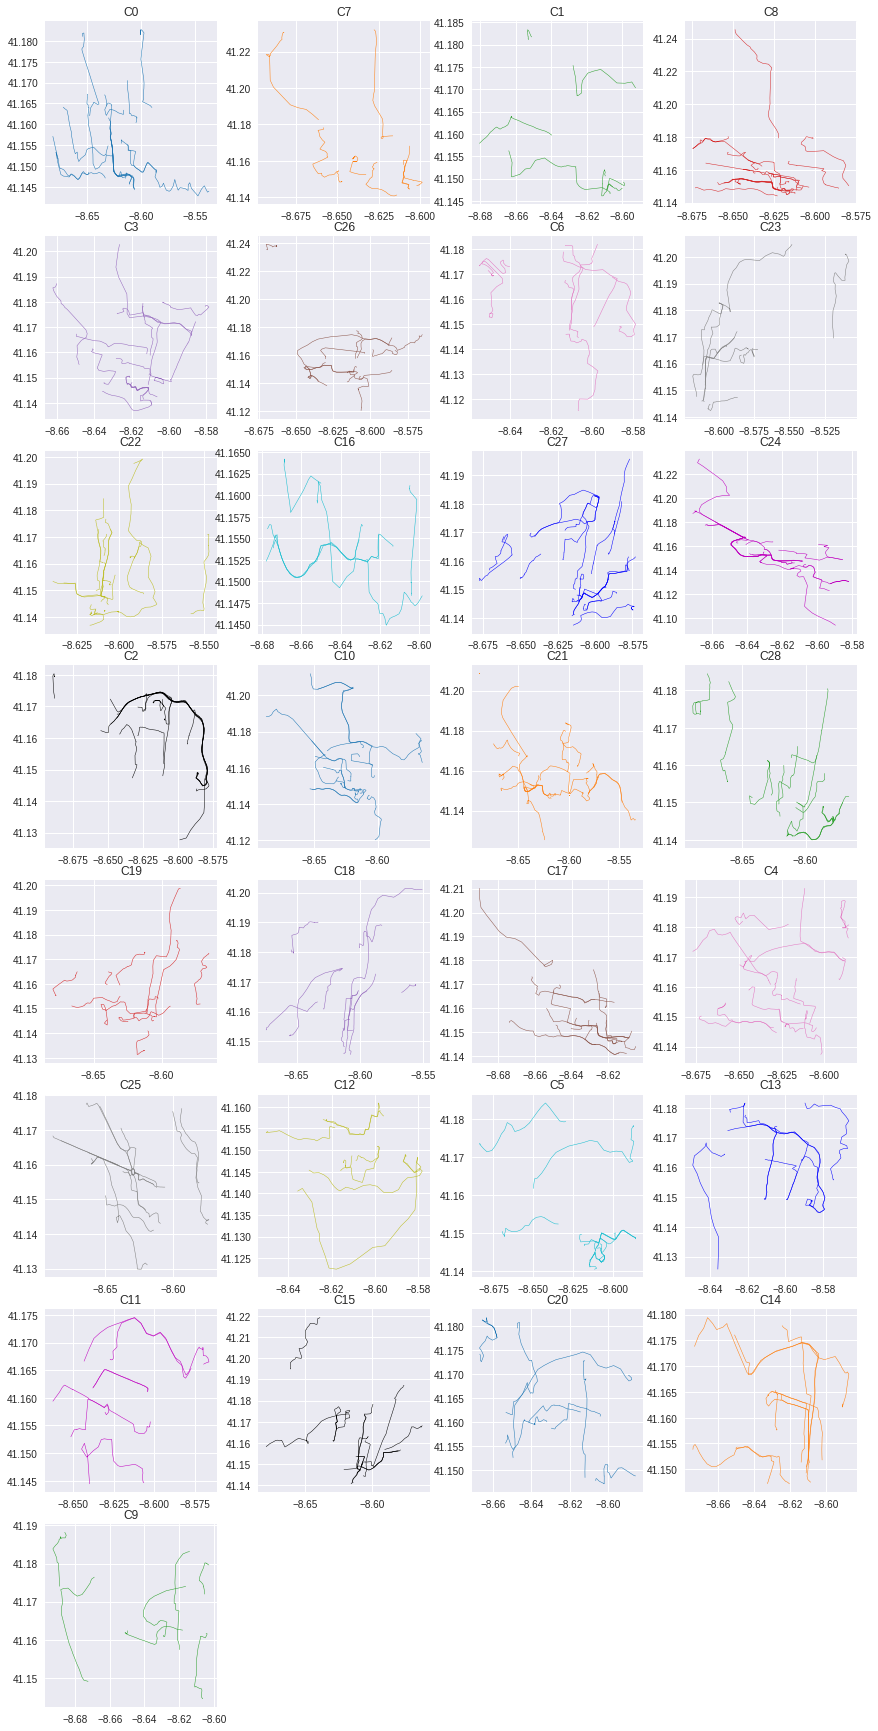
\includegraphics[width=.9\linewidth,height=.9\textheight,keepaspectratio]{figs/clusters/CLU_AP_ALL[SSPD]_REAL.png}
  \caption{Affinity propagation clusters created with SSPD, but showing the raw trajectory locations}
  \label{fig:sspd_loc_real}
\end{figure}


\subsection{Distance Computation and Evaluation}
% Tweaking the format and scale of the data is one thing, but the next line of simplifications mattered more for the evaluations of the measures. 

We tested three measures that required a parameter and we did not do any proper parameter tuning. 
ERP would likely have had more agreement with the other measures in \Cref{tab:top-10-sim-pairs} if different values for the reference point had been tested out. 


% Next, while we did not  the measues 

% The last simplification we would like to bring attention to is also something that potentially affected the final evaluation. 

The application we chose for the similarity distance measures, clustering, is itself an area of active research. 
The interconnectedness of clustering techniques and distance algorithms could have been studied in more detail before settling on affinity propagation and hierarchical clustering analysis as the evaluation basis.
We acknowledge that there may be traits of the selected measures that have been obscured or misrepresented. 


\chapter{Conclusion and Further Work}
\label{ch:8}

\section{Conclusion}

% In this thesis we studied how the data format of trajectories and outlined seven different approaches for quantifying the similarity distance between them. After describing how each of the algorithms were designed, a set up was created so for experimentally comparing them. A data set and an application of similarity scores were chosen so that the effects of the distance measure could be as isolated as possible for a perceptible comparison. 

In this thesis, we studied seven similarity measures for trajectory data, five conventional ones and two recent ones. 
First, we clarified what constitutes a trajectory, and then we discussed how the notion of similarity of them varies.
The measures we reviewed vary in how they defined similarity and we elaborated upon some of their advantages and disadvantages. 

In order to experimentally compare the algorithms, we defined an application wherein the only thing that varied was the similarity distance computation. 
The application we decided on was clustering and we used two techniques for creating them.
The clusters gave us a vantage point for further description of the measures, and from the clusters, we were able to observe the theoretical characteristics of the measures in practice. 
We summarize what has been achieved in this thesis by referring back to the research objectives:



\subsubsection*{Research Objectives 1 and 2:} 
The conventional similarity measures we examined were the Euclidean distance, Dynamic Time Warping, Hausdorff Distance, Edit Distance on Real Sequence, and Edit distance with Real Penalty. 
The latter two are newer than the other ones, however, their prominence in the literature establishes them as conventional methods. 
A commonality between these measures is that they are not context-aware. 
In terms of noise tolerance, there was no consistency, and as for elasticity all but Ed are could adapt to local time shifts. 

Both Move-Split-Merge and Symmetric Segment Path Distance are methods that were developed in order to address the shortcomings of the conventional methods.
Based on this we categorized them as the newer distance measures. 


\clearpage
The development of MSM was a response to DTW and ERP while SSPD was an advancement of Hd.
A feature that is shared between MSM and SSPD is that they both were designed to account for whole trajectory similarity.
Additionally, they are more tolerant to noise than their respective conventional method inspirations.
We saw this experimentally as MSM producing crisper clusterings than DTW and ERP and SSPD producing crisper clusterings than Hd.

We were not able to determine any effects of metricity, neither for the conventional methods nor for the newer ones. 
For the visual representation of how trajectory features were treated by the we refer to \Cref{app:ap-clu,app:h-clu}  


\subsubsection*{Research Objective 3:}
In our set up, there was only one application that tested the algorithms’ performance against each other. 
The lack of diverse applications and their removal from real-world observations are limiting how much insight we could gain regarding broader uses for the measures. Nevertheless, the variance of the cluster we generated demonstrates that similarity distance measure choice matters.

 We could have constructed arguments that would have framed a given measure as the most suited one for shape-based clustering. However, we reiterate could not have generalized its applicability to other tasks.

Optimizing for global shape-similarity should be prioritized if the intended application is computer vision or migration analysis.  
On the other hand, locally shifted similarities are needed for database management tasks such as outlier detection and trajectory uncertainty. An outlier in this context could be either a trajectory element that stands out from its surrounding elements or a trajectory that stands out from the rest. Trajectory uncertainty management seeks to increase the utility of trajectories by approximating locations between observations. 
In both cases, a reference model of local resemblance is more apt.  

Consequently, we remark that the accuracy and reliability of analysis or management tasks depend on whether or not an appropriate algorithm was chosen. 



% In terms of usage for different applications here was only one application in this thesis. While being limiting for the insight we gathered it was enough to demonstrate that choice matters. All methods described were supposedly spatial-only trajectory similarity but the results they gave varied a lot – this point further supports the theory of there not being a ground truth of what similarity is for time-series. 
% e
% Algorithm selection had a substantial influence over the results, even in this scaled down experiment. We argue that one should not picking a method purely on the basis of it being prominent in the literature as it may biases that are not evident from the description resulting in misleading findings. 

\clearpage
\section{Further Work}

% The work done in thesis a good foundation for more experiment.
The work we have done for this thesis explored just one class of trajectory similarity and one particular application for similarity measures.
There are aspects of trajectory similarity we did not inquire into. 
Thus we suggest two extensions of our experiment which would facilitate a more comprehensive study. 


% Larger data set, longer trajectories (trajectories that have not been arifically shortened), both.
As we noted in \Cref{ch:5}, our set up was not conducive to examining the differences in computational complexity. 
If it were possible, we would have liked to include an evaluation of measures’ performances; both for the data set used here and sets where the lengths of the trajectories had not been artificially shortened. 
As with most algorithms, it is good to be informed about how they will perform as the size of the data or the data set increases.



% There are are would be conductive to a more comprehensive study of trajectory similarly.
It would make sense to include more applications for the measures.
Along with clustering, classification is a commonly selected application for testing the measures. 
However, we argue it would be interesting to run either an outlier detection or noise removal task. 
This could hopefully highlight peculiarities of how the measures distinguish the trajectories.




% \subsection{Thematic Areas for Continued Research}




\chapter*{\bibname}
\printbibliography[heading=none]

\appendix

\chapter{Most Similar Trajectory Pairs }
\label{app:simtab}

\begin{landscape}
{
\scriptsize
\tabcolsep=2.5pt  % hold it local
\renewcommand{\arraystretch}{1.1}

\begin{longtable}{ccccccccccc}

% 'ccccccccccc' lllllllllll
\caption{Raking of most similar trajectory pairs}                                
\label{app:tab:top50}\\
\toprule
  \textbf{Rank} & 
  \textbf{Euclidean} &
  \textbf{DTW} &
  \textbf{SSPD} &
  \textbf{Hausdorff} &
  \textbf{ERP} &
  \textbf{MSM; cost=1} &
  \textbf{MSM; cost=.1} &
  \textbf{MSM; cost=.01} &
  \textbf{EDR; $\epsilon=.203$} &
  \textbf{EDR; $\epsilon=.101$} \\
\hline          
\endhead
% \midrule
\multicolumn{11}{c}{{}} \\
\midrule
\multicolumn{11}{c}{{Continued on next page}} \\
\midrule
\endfoot
% \bottomrule
\endlastfoot
1  &  QREOR-IHNMX &  LFQDH-ACJIG &  LFQDH-ACJIG &  NVZCQ-TGKDX &  QREOR-IHNMX &  QREOR-IHNMX &  QREOR-IHNMX &  LFQDH-ACJIG &  LFQDH-ACJIG &  LFQDH-ACJIG \\
2  &  LFQDH-ACJIG &  NVZCQ-TGKDX &  KQQUG-OVNBK &  QREOR-IHNMX &  LFQDH-ACJIG &  LFQDH-ACJIG &  LFQDH-ACJIG &  NVZCQ-TGKDX &  WBTAG-QMRPP &  QREOR-IHNMX \\
3  &  BZCYT-VXLBC &  QREOR-IHNMX &  QREOR-IHNMX &  LFQDH-ACJIG &  BZCYT-VXLBC &  BZCYT-VXLBC &  NVZCQ-TGKDX &  KQQUG-OVNBK &  BLHVW-ATPTV &  KQQUG-OVNBK \\
4  &  LHTXJ-TGKDX &  KQQUG-OVNBK &  NVZCQ-TGKDX &  KQQUG-OVNBK &  LHTXJ-TGKDX &  LHTXJ-TGKDX &  BZCYT-VXLBC &  QREOR-IHNMX &  TNPJQ-LRZLR &  NVZCQ-TGKDX \\
5  &  PSVVR-XSJJE &  LHTXJ-TGKDX &  LHTXJ-TGKDX &  OVNBK-GRPNX &  PSVVR-XSJJE &  PSVVR-XSJJE &  KQQUG-OVNBK &  LHTXJ-TGKDX &  UHLAI-WFZIE &  PSVVR-XSJJE \\
6  &  NVZCQ-TGKDX &  BZCYT-VXLBC &  LVFYZ-SYVIQ &  OKPGU-FZIOY &  NVZCQ-TGKDX &  NVZCQ-TGKDX &  LHTXJ-TGKDX &  LVFYZ-SYVIQ &  XXVQK-LOBQA &  BZCYT-VXLBC \\
7  &  TNPJQ-LRZLR &  OVNBK-GRPNX &  BZCYT-VXLBC &  PSVVR-XSJJE &  TNPJQ-LRZLR &  TNPJQ-LRZLR &  PSVVR-XSJJE &  PSVVR-XSJJE &  XLLLQ-OKPGU &  HUSJF-UHLAI \\
8  &  HUSJF-UHLAI &  LVFYZ-SYVIQ &  OVNBK-GRPNX &  WBTAG-QMRPP &  HUSJF-UHLAI &  HUSJF-UHLAI &  HUSJF-UHLAI &  BZCYT-VXLBC &  OKPGU-FZIOY &  LHTXJ-TGKDX \\
9  &  ZQZSA-NVZCQ &  PSVVR-XSJJE &  HUSJF-UHLAI &  BZCYT-VXLBC &  ZQZSA-NVZCQ &  ZQZSA-NVZCQ &  OVNBK-GRPNX &  NVZCQ-LHTXJ &  HUSJF-UHLAI &  IQXOG-LENWX \\
10 &  NVZCQ-TNPJQ &  HUSJF-UHLAI &  PSVVR-XSJJE &  HUSJF-UHLAI &  NVZCQ-TNPJQ &  NVZCQ-TNPJQ &  NVZCQ-LHTXJ &  OVNBK-GRPNX &  NKEGR-VXLBC &  OVNBK-GRPNX \\
11 &  OVNBK-GRPNX &  LRZLR-BFFJE &  LRZLR-BFFJE &  UHLAI-WFZIE &  OVNBK-GRPNX &  OVNBK-GRPNX &  NVZCQ-TNPJQ &  LRZLR-BFFJE &  LHTXJ-TGKDX &  GELAB-TVLNM \\
12 &  BLHVW-ATPTV &  NVZCQ-LHTXJ &  NVZCQ-LHTXJ &  IQXOG-LENWX &  BLHVW-ATPTV &  BLHVW-ATPTV &  ZKNAC-QMRPP &  HUSJF-UHLAI &  QREOR-IHNMX &  BLHVW-ATPTV \\
13 &  BZCYT-NKEGR &  ZKNAC-QMRPP &  ZKNAC-QMRPP &  NVZCQ-LRZLR &  BZCYT-NKEGR &  BZCYT-NKEGR &  BLHVW-ATPTV &  NVZCQ-LRZLR &  PSVVR-XSJJE &  ZKNAC-QMRPP \\
14 &  IQXOG-LENWX &  NVZCQ-BFFJE &  IQXOG-LENWX &  LHTXJ-TGKDX &  IQXOG-LENWX &  IQXOG-LENWX &  LVFYZ-SYVIQ &  NVZCQ-TNPJQ &  LRZLR-JKBML &  NVZCQ-LHTXJ \\
15 &  UHLAI-WFZIE &  NVZCQ-TNPJQ &  NVZCQ-TNPJQ &  NVZCQ-LHTXJ &  UHLAI-WFZIE &  UHLAI-WFZIE &  IQXOG-LENWX &  LDASI-HUSJF &  OVNBK-GRPNX &  ZQZSA-NVZCQ \\
16 &  XLLLQ-OKPGU &  IQXOG-LENWX &  LDASI-HUSJF &  NVZCQ-BFFJE &  XLLLQ-OKPGU &  XLLLQ-OKPGU &  NVZCQ-LRZLR &  ZKNAC-QMRPP &  GPQBK-JBHAY &  NVZCQ-LRZLR \\
17 &  IXPBX-QQOCG &  NVZCQ-LRZLR &  NVZCQ-BFFJE &  XXVQK-LOBQA &  IXPBX-QQOCG &  IXPBX-QQOCG &  ZQZSA-NVZCQ &  BZCYT-NKEGR &  VZJTC-PEICU &  LDASI-UHLAI \\
18 &  LRZLR-JKBML &  BLHVW-ATPTV &  BLHVW-ATPTV &  ZKNAC-QMRPP &  LRZLR-JKBML &  LRZLR-JKBML &  LDASI-HUSJF &  NVZCQ-BFFJE &  BZCYT-VXLBC &  GPQBK-JBHAY \\
19 &  KQQUG-OVNBK &  WBTAG-QMRPP &  XXVQK-LOBQA &  VZJTC-PEICU &  KQQUG-OVNBK &  KQQUG-OVNBK &  GPQBK-JBHAY &  IQXOG-LENWX &  MSSZC-GNPOB &  LVFYZ-SYVIQ \\
20 &  WBTAG-QMRPP &  BZCYT-NKEGR &  NVZCQ-LRZLR &  LRZLR-JKBML &  WBTAG-QMRPP &  WBTAG-QMRPP &  TNPJQ-LRZLR &  HUSJF-WFZIE &  ZQZSA-TGKDX &  LRZLR-JKBML \\
21 &  VZJTC-PEICU &  TNPJQ-LRZLR &  MSSZC-GNPOB &  BLHVW-ATPTV &  VZJTC-PEICU &  VZJTC-PEICU &  IXPBX-QQOCG &  OKPGU-FZIOY &  BZCYT-NKEGR &  NVZCQ-TNPJQ \\
22 &  BXHSU-DRZGY &  GPQBK-JBHAY &  ZJFVA-VXLBC &  LVFYZ-SYVIQ &  BXHSU-DRZGY &  BXHSU-DRZGY &  BZCYT-NKEGR &  ZQZSA-NVZCQ &  NVZCQ-LRZLR &  TNPJQ-LRZLR \\
23 &  GPQBK-JBHAY &  IXPBX-QQOCG &  HUSJF-WFZIE &  MSSZC-GNPOB &  GPQBK-JBHAY &  GPQBK-JBHAY &  LDASI-UHLAI &  VZJTC-PEICU &  NVZCQ-LHTXJ &  LDASI-HUSJF \\
24 &  NVZCQ-LRZLR &  XXVQK-LOBQA &  TNPJQ-LRZLR &  XLLLQ-OKPGU &  NVZCQ-LRZLR &  NVZCQ-LRZLR &  XLLLQ-OKPGU &  XLLLQ-OKPGU &  HUSJF-WFZIE &  VZJTC-PEICU \\
25 &  MSSZC-GNPOB &  LDASI-HUSJF &  IXPBX-QQOCG &  WBTAG-VIBJH &  MSSZC-GNPOB &  MSSZC-GNPOB &  UHLAI-WFZIE &  NKEGR-VXLBC &  LDASI-UHLAI &  XLLLQ-OKPGU \\
26 &  LDASI-UHLAI &  UHLAI-WFZIE &  WBTAG-QMRPP &  IQXOG-LVFYZ &  LDASI-UHLAI &  LDASI-UHLAI &  LRZLR-BFFJE &  IXPBX-QQOCG &  ZKNAC-QMRPP &  WBTAG-QMRPP \\
27 &  GELAB-TVLNM &  ZQZSA-NVZCQ &  ZBJPA-BMJXU &  NKEGR-VXLBC &  GELAB-TVLNM &  GELAB-TVLNM &  HUSJF-WFZIE &  WBTAG-VIBJH &  TSOBU-MIRVW &  IXPBX-QQOCG \\
28 &  ZQZSA-TGKDX &  XLLLQ-OKPGU &  UHLAI-WFZIE &  ZQZSA-NVZCQ &  ZQZSA-TGKDX &  ZQZSA-TGKDX &  NVZCQ-BFFJE &  BXHSU-DRZGY &  IXPBX-QQOCG &  ZBJPA-BMJXU \\
29 &  WBTAG-VIBJH &  MSSZC-GNPOB &  BZCYT-NKEGR &  LRZLR-BFFJE &  WBTAG-VIBJH &  WBTAG-VIBJH &  XXVQK-LOBQA &  XXVQK-LOBQA &  WBTAG-VIBJH &  UTNLD-XSJJE \\
30 &  IQXOG-LVFYZ &  HUSJF-WFZIE &  LDASI-UHLAI &  TNPJQ-LRZLR &  IQXOG-LVFYZ &  IQXOG-LVFYZ &  VZJTC-PEICU &  UHLAI-WFZIE &  BXHSU-DRZGY &  HUSJF-WFZIE \\
31 &  OKPGU-FZIOY &  OKPGU-FZIOY &  OKPGU-FZIOY &  BXHSU-DRZGY &  OKPGU-FZIOY &  OKPGU-FZIOY &  BXHSU-DRZGY &  TNPJQ-LRZLR &  IQXOG-LVFYZ &  BZCYT-NKEGR \\
32 &  LDASI-HUSJF &  VZJTC-PEICU &  BZCYT-ZJFVA &  BZCYT-NKEGR &  LDASI-HUSJF &  LDASI-HUSJF &  LRZLR-JKBML &  BLHVW-ATPTV &  NVZCQ-TNPJQ &  BXHSU-DRZGY \\
33 &  XXVQK-LOBQA &  LRZLR-JKBML &  GPQBK-JBHAY &  HUSJF-WFZIE &  XXVQK-LOBQA &  XXVQK-LOBQA &  MSSZC-GNPOB &  ZBJPA-BMJXU &  IQXOG-LENWX &  UHLAI-WFZIE \\
34 &  ZJFVA-VXLBC &  LDASI-UHLAI &  VKGQV-BLHVW &  AEPAP-XLLLQ &  ZJFVA-VXLBC &  ZJFVA-VXLBC &  ZQZSA-TGKDX &  WBTAG-QMRPP &  NVZCQ-TGKDX &  ZQZSA-TGKDX \\
35 &  ZKNAC-QMRPP &  WBTAG-VIBJH &  XLLLQ-OKPGU &  VKGQV-BLHVW &  ZKNAC-QMRPP &  ZKNAC-QMRPP &  WBTAG-QMRPP &  LDASI-UHLAI &  LRZLR-BFFJE &  MSSZC-GNPOB \\
36 &  NKEGR-VXLBC &  ZBJPA-BMJXU &  WBTAG-VIBJH &  BZCYT-ZJFVA &  NKEGR-VXLBC &  NKEGR-VXLBC &  ZBJPA-BMJXU &  QQOCG-FIJTA &  KQQUG-OVNBK &  TSOBU-MIRVW \\
37 &  VKGQV-BLHVW &  NKEGR-VXLBC &  VZJTC-PEICU &  GPQBK-JBHAY &  VKGQV-BLHVW &  VKGQV-BLHVW &  WBTAG-VIBJH &  LRZLR-JKBML &  LVFYZ-SYVIQ &  NVZCQ-BFFJE \\
38 &  NVZCQ-LHTXJ &  BXHSU-DRZGY &  ZQZSA-NVZCQ &  IXPBX-QQOCG &  NVZCQ-LHTXJ &  NVZCQ-LHTXJ &  VKGQV-BLHVW &  GPQBK-JBHAY &  ZQZSA-NVZCQ &  VKGQV-BLHVW \\
39 &  LRZLR-BFFJE &  ZQZSA-TGKDX &  AEPAP-XLLLQ &  ZQZSA-TGKDX &  LRZLR-BFFJE &  LRZLR-BFFJE &  GELAB-TVLNM &  MSSZC-GNPOB &  NVZCQ-BFFJE &  AEPAP-XLLLQ \\
40 &  AEPAP-XLLLQ &  VKGQV-BLHVW &  LRZLR-JKBML &  GELAB-TVLNM &  AEPAP-XLLLQ &  AEPAP-XLLLQ &  BZCYT-ZJFVA &  ZJFVA-VXLBC &  QQOCG-FIJTA &  BZCYT-ZJFVA \\
41 &  HUSJF-WFZIE &  BZCYT-ZJFVA &  BLHVW-VPCTJ &  QQOCG-FIJTA &  HUSJF-WFZIE &  HUSJF-WFZIE &  OKPGU-FZIOY &  AEPAP-XLLLQ &  AEPAP-XLLLQ &  XXVQK-LOBQA \\
42 &  NVZCQ-BFFJE &  UTNLD-XSJJE &  BXHSU-DRZGY &  BLHVW-VPCTJ &  NVZCQ-BFFJE &  NVZCQ-BFFJE &  UTNLD-XSJJE &  VKGQV-BLHVW &  LDASI-HUSJF &  LRZLR-BFFJE \\
43 &  QQOCG-FIJTA &  AEPAP-XLLLQ &  NKEGR-VXLBC &  NVZCQ-TNPJQ &  QQOCG-FIJTA &  QQOCG-FIJTA &  BLHVW-VPCTJ &  BZCYT-ZJFVA &  GELAB-TVLNM &  WBTAG-VIBJH \\
44 &  TSOBU-MIRVW &  ZJFVA-VXLBC &  ZQZSA-TGKDX &  ZJFVA-VXLBC &  TSOBU-MIRVW &  TSOBU-MIRVW &  NKEGR-VXLBC &  ZQZSA-TGKDX &  BZCYT-LPNRG &  BLHVW-VPCTJ \\
45 &  BZCYT-ZJFVA &  BLHVW-VPCTJ &  QQOCG-FIJTA &  BZCYT-LPNRG &  LVFYZ-SYVIQ &  BZCYT-ZJFVA &  IQXOG-LVFYZ &  IQXOG-LVFYZ &  ZBJPA-BMJXU &  ZJFVA-VXLBC \\
46 &  LVFYZ-SYVIQ &  QQOCG-FIJTA &  GELAB-TVLNM &  LDASI-UHLAI &  BZCYT-ZJFVA &  LVFYZ-SYVIQ &  ZJFVA-VXLBC &  BLHVW-VPCTJ &  UTNLD-XSJJE &  IQXOG-LVFYZ \\
47 &  BZCYT-LPNRG &  IQXOG-LVFYZ &  IQXOG-LVFYZ &  TSOBU-MIRVW &  BZCYT-LPNRG &  BZCYT-LPNRG &  TSOBU-MIRVW &  GELAB-TVLNM &  VKGQV-BLHVW &  OKPGU-FZIOY \\
48 &  UTNLD-XSJJE &  GELAB-TVLNM &  UTNLD-XSJJE &  ZBJPA-BMJXU &  UTNLD-XSJJE &  UTNLD-XSJJE &  QQOCG-FIJTA &  BZCYT-LPNRG &  BZCYT-ZJFVA &  QQOCG-FIJTA \\
49 &  BLHVW-VPCTJ &  TSOBU-MIRVW &  TSOBU-MIRVW &  LDASI-HUSJF &  BLHVW-VPCTJ &  BLHVW-VPCTJ &  AEPAP-XLLLQ &  TSOBU-MIRVW &  BLHVW-VPCTJ &  BZCYT-LPNRG \\
50 &  ZBJPA-BMJXU &  BZCYT-LPNRG &  BZCYT-LPNRG &  UTNLD-XSJJE &  ZBJPA-BMJXU &  ZBJPA-BMJXU &  BZCYT-LPNRG &  UTNLD-XSJJE &  ZJFVA-VXLBC &  NKEGR-VXLBC \\
\end{longtable}
}
\end{landscape}

\chapter{Affinity Propagation Clusters}
\label{app:ap-clu}

\begin{figure}[h]
  \centering
  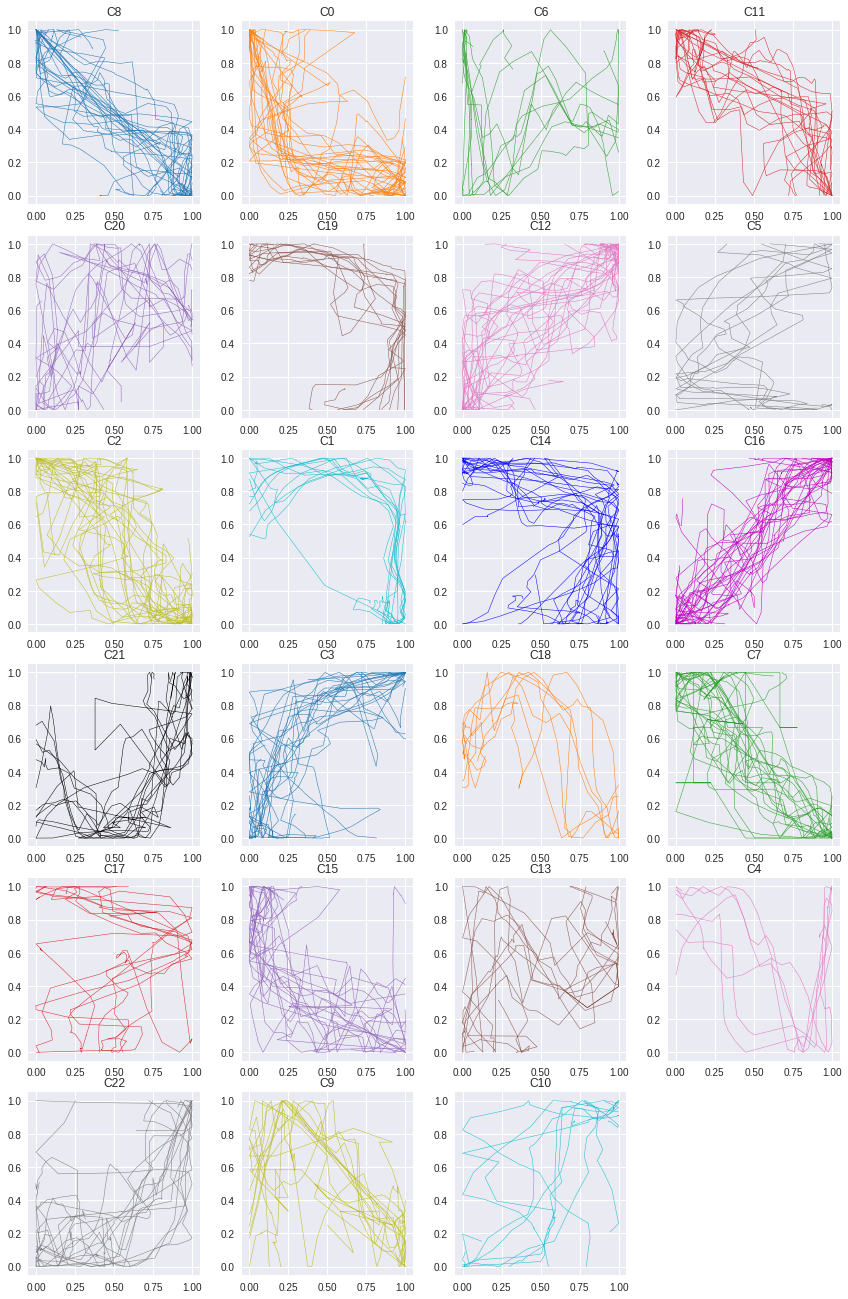
\includegraphics[width=\linewidth,height=\textheight,keepaspectratio]{figs/clusters/CLU_AP_ALL[DTW].png}
  \caption{Affinity Propagation: Dynamic Time Warping}
\end{figure}

\begin{figure}[h]
  \centering
  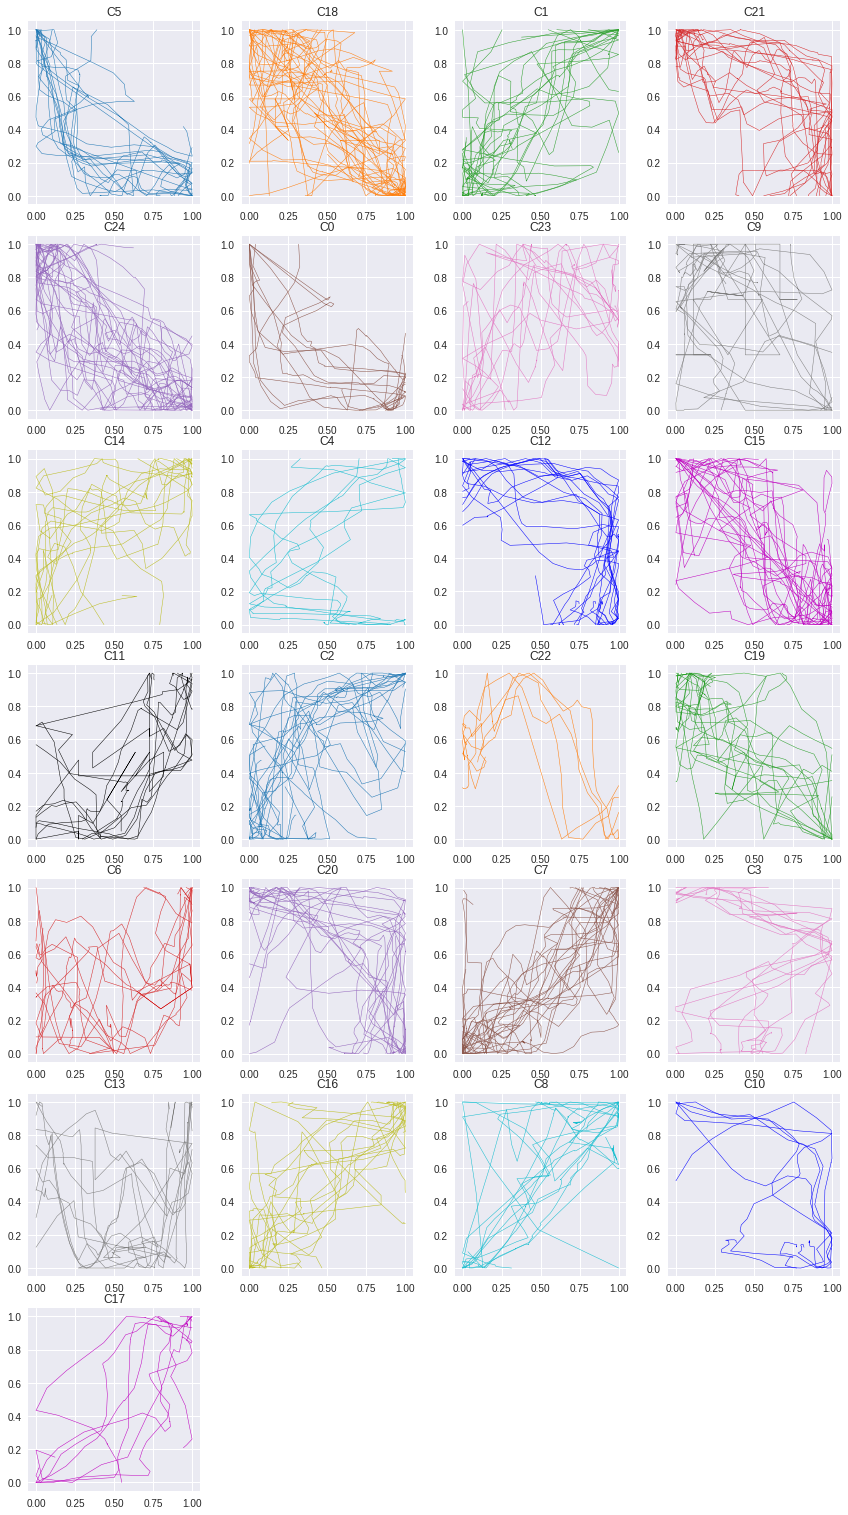
\includegraphics[width=\linewidth,height=\textheight,keepaspectratio]{figs/clusters/CLU_AP_ALL[Ed].png}
  \caption{Affinity Propagation: Euclidean Distance}
\end{figure}

\begin{figure}[h]
  \centering
  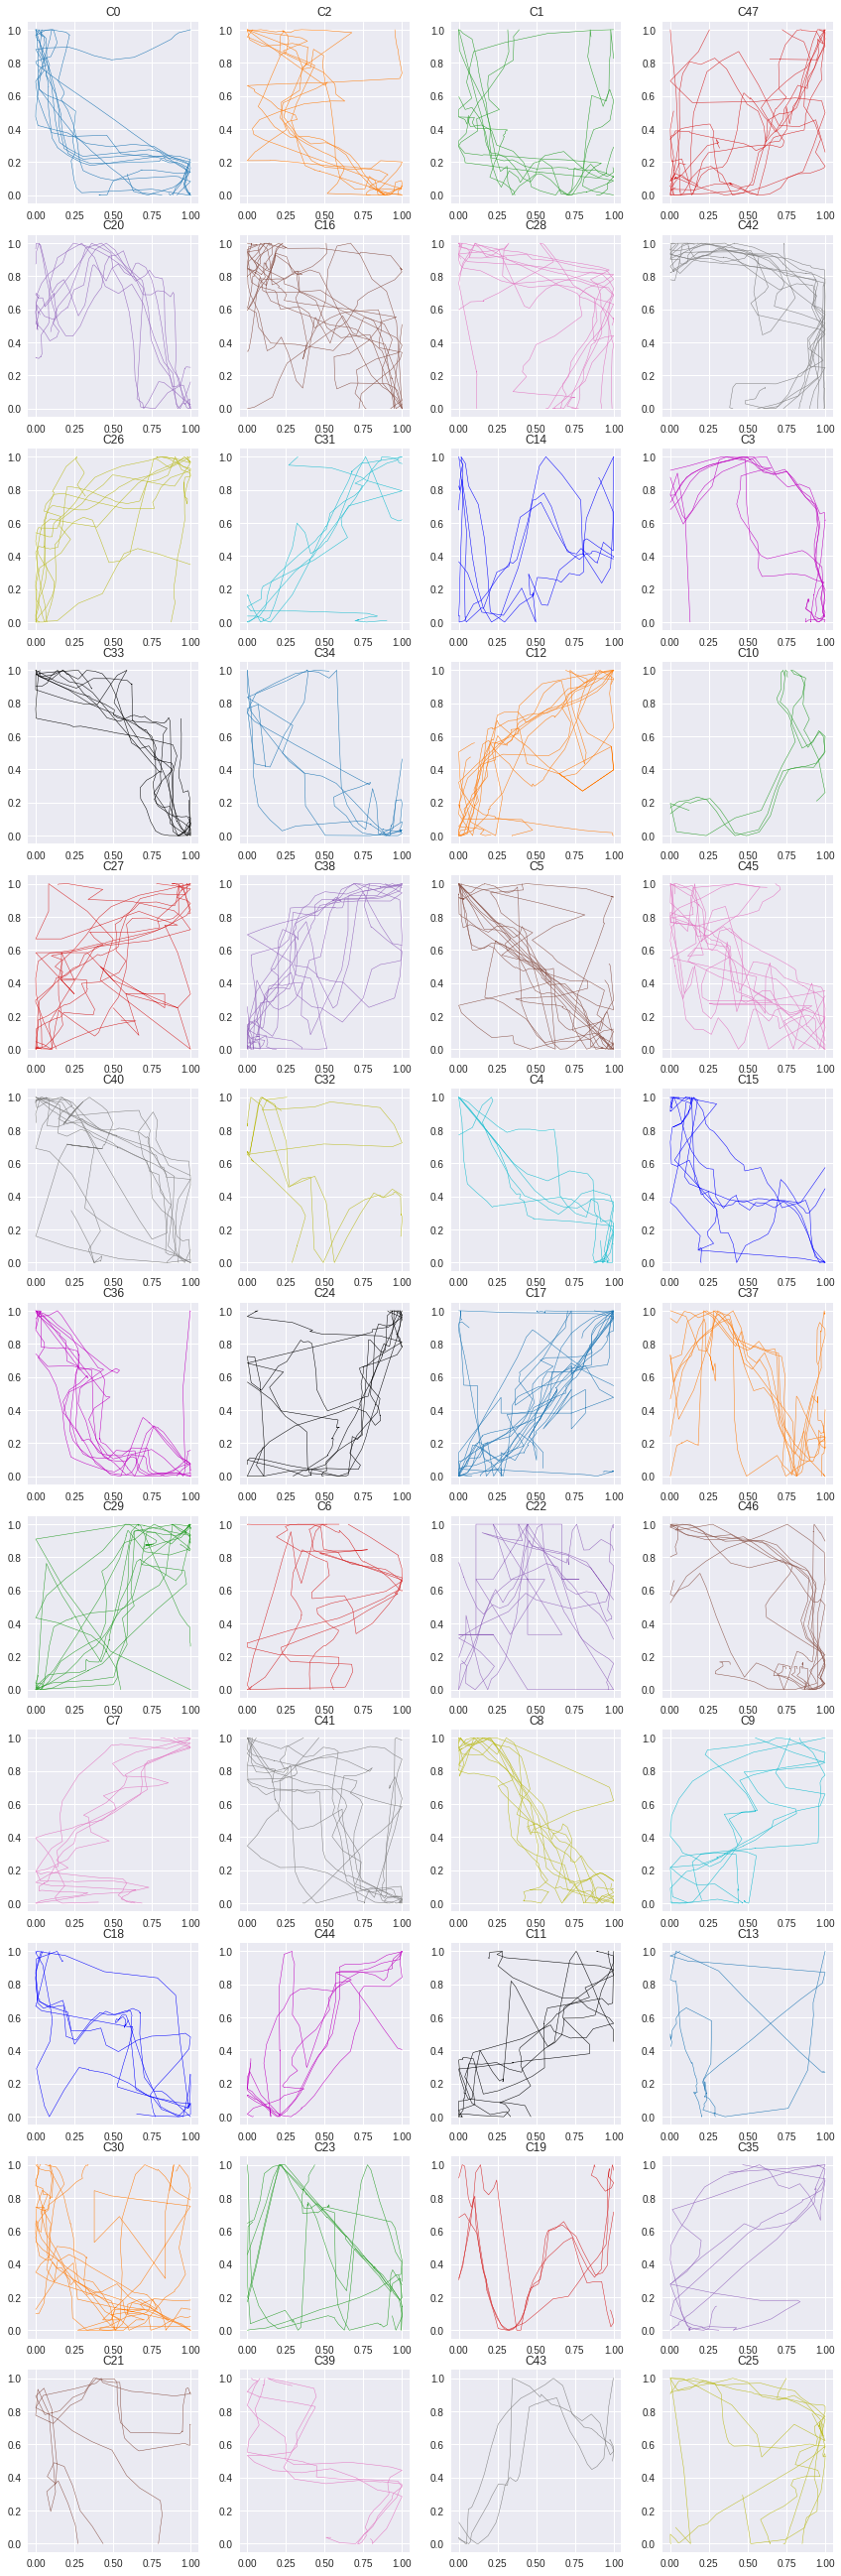
\includegraphics[width=\linewidth,height=\textheight,keepaspectratio]{figs/clusters/CLU_AP_ALL[EDR;e=.101].png}
  \caption{Affinity Propagation: Edit Distance on Real Sequence, $\epsilon=0.101$}
\end{figure}

\begin{figure}[h]
  \centering
  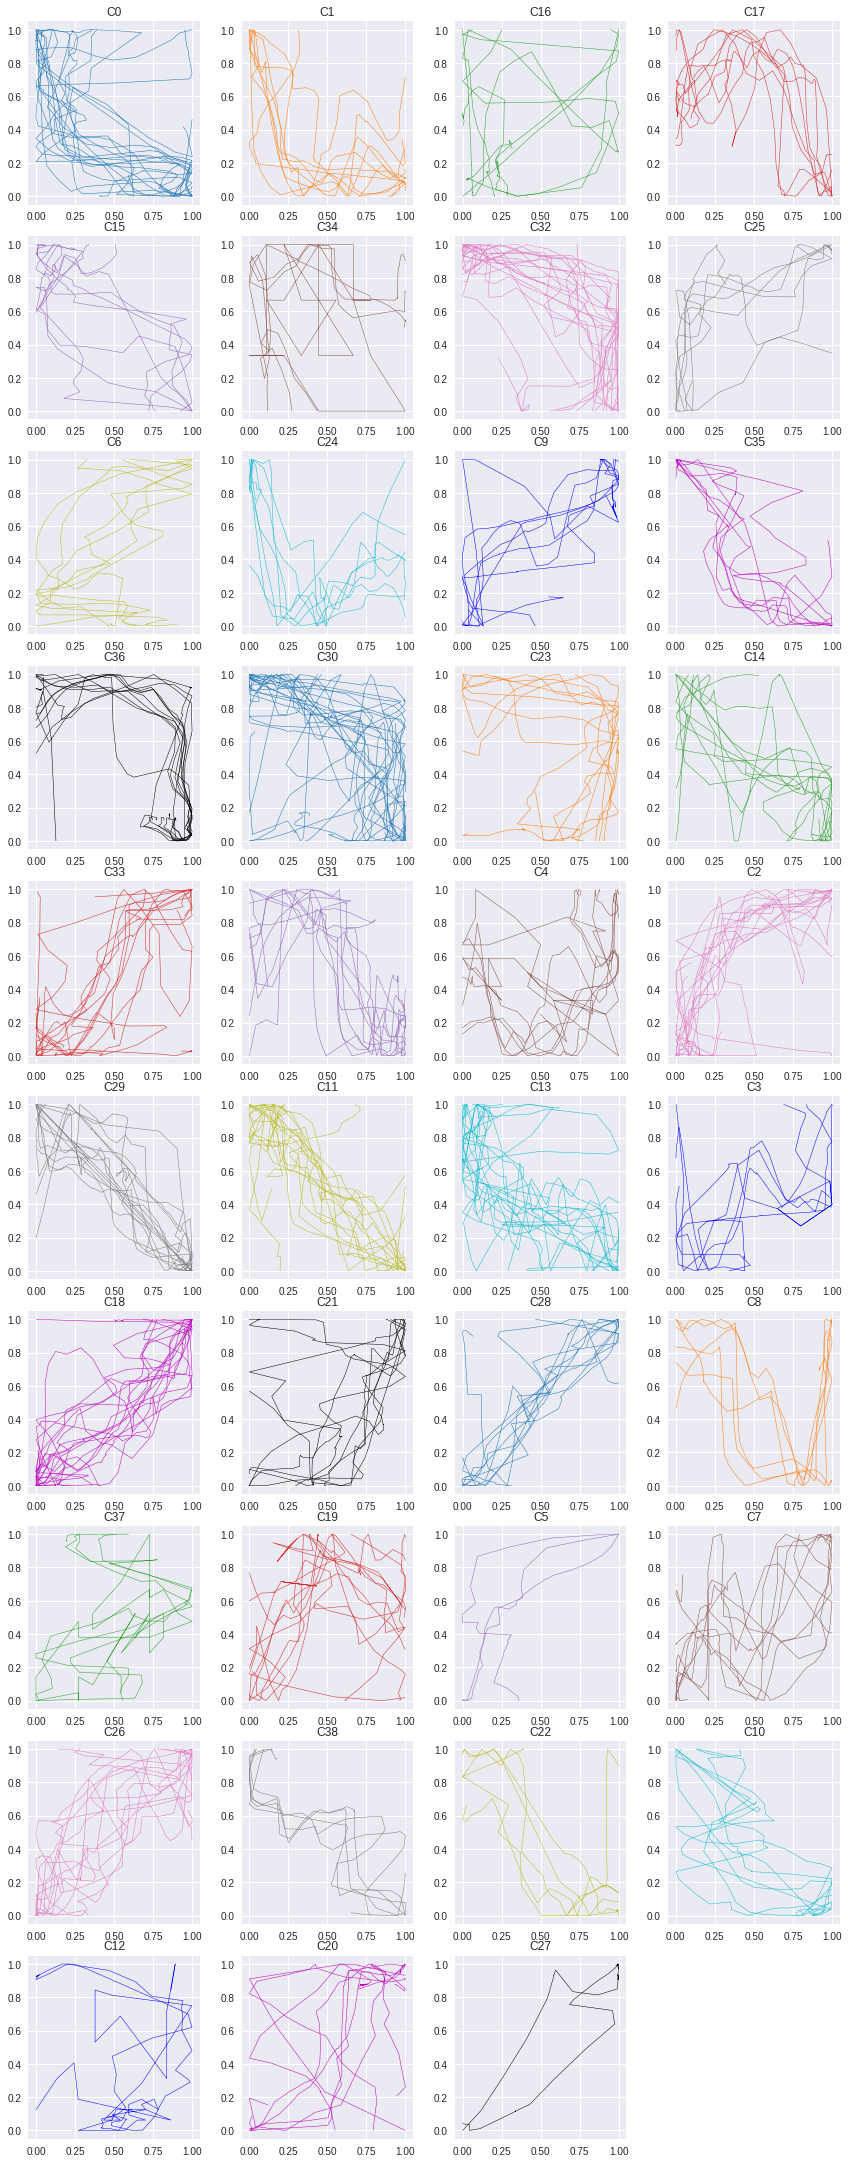
\includegraphics[width=\linewidth,height=\textheight,keepaspectratio]{figs/clusters/CLU_AP_ALL[EDR;e=.203].png}
  \caption{Affinity Propagation: Edit Distance on Real Sequence, $\epsilon=0.203$}
\end{figure}

\begin{figure}[h]
  \centering
  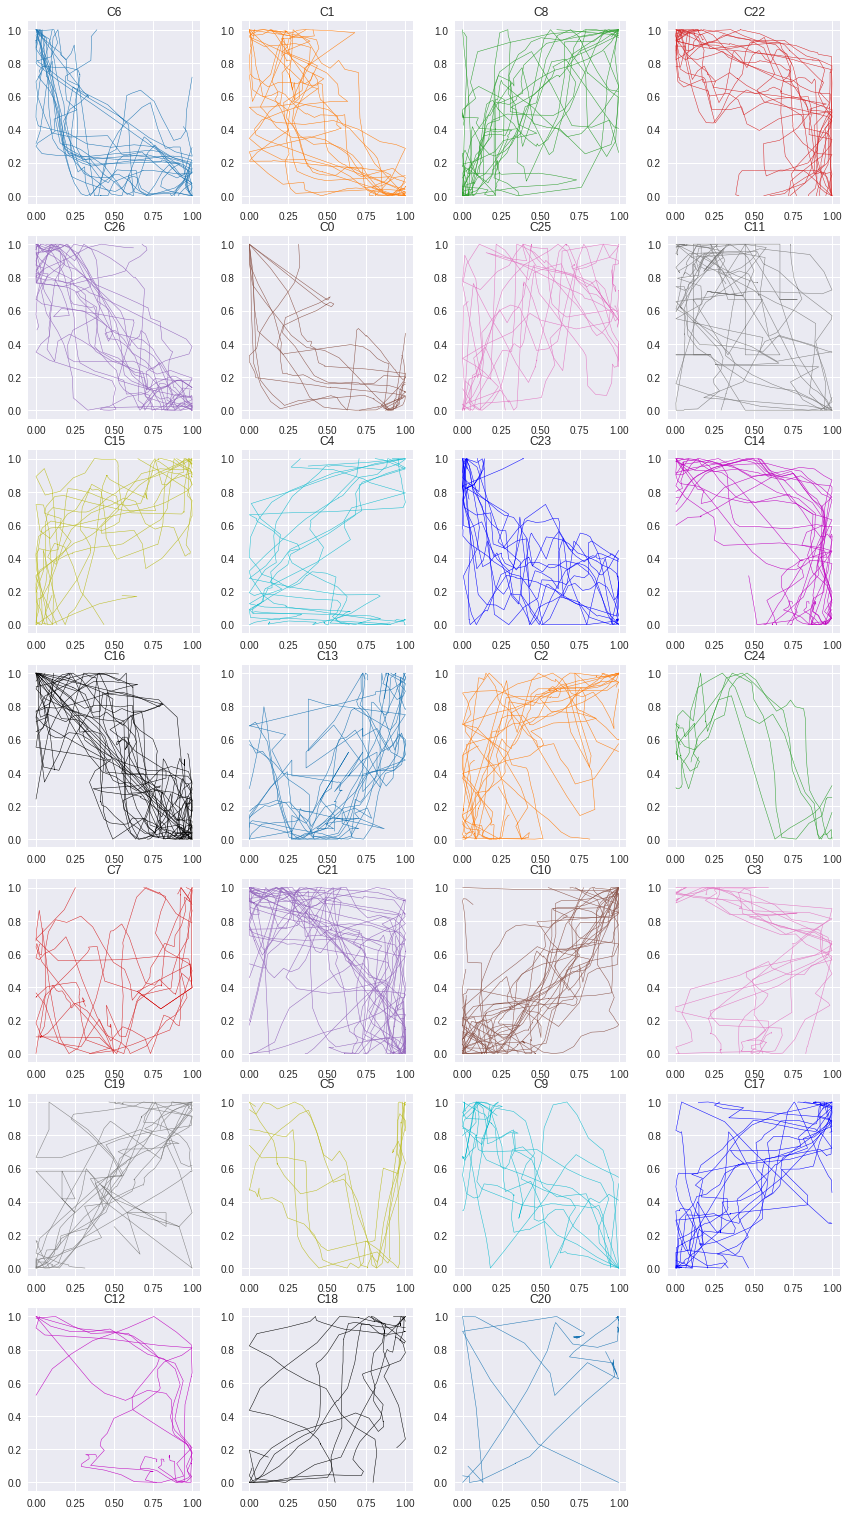
\includegraphics[width=\linewidth,height=\textheight,keepaspectratio]{figs/clusters/CLU_AP_ALL[ERP;g=0,0].png}
  \caption{Affinity Propagation: Edit Distance with Real Penalty}
\end{figure}

\begin{figure}[h]
  \centering
  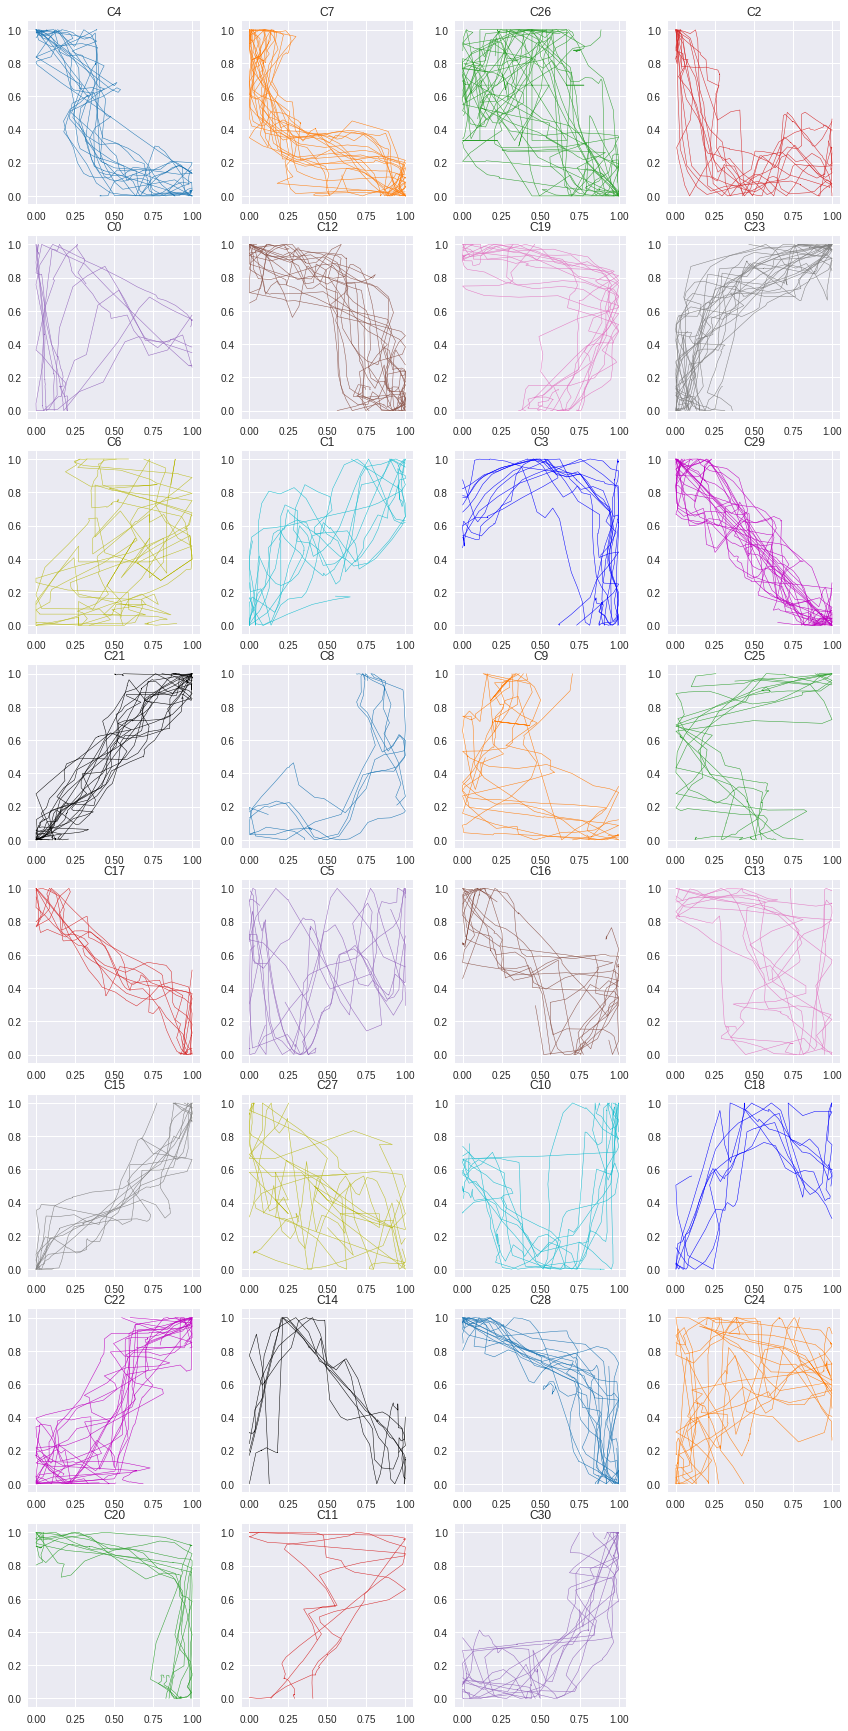
\includegraphics[width=\linewidth,height=\textheight,keepaspectratio]{figs/clusters/CLU_AP_ALL[Hd].png}
  \caption{Affinity Propagation: Hausdorff Distance}
\end{figure}

\begin{figure}[h]
  \centering
  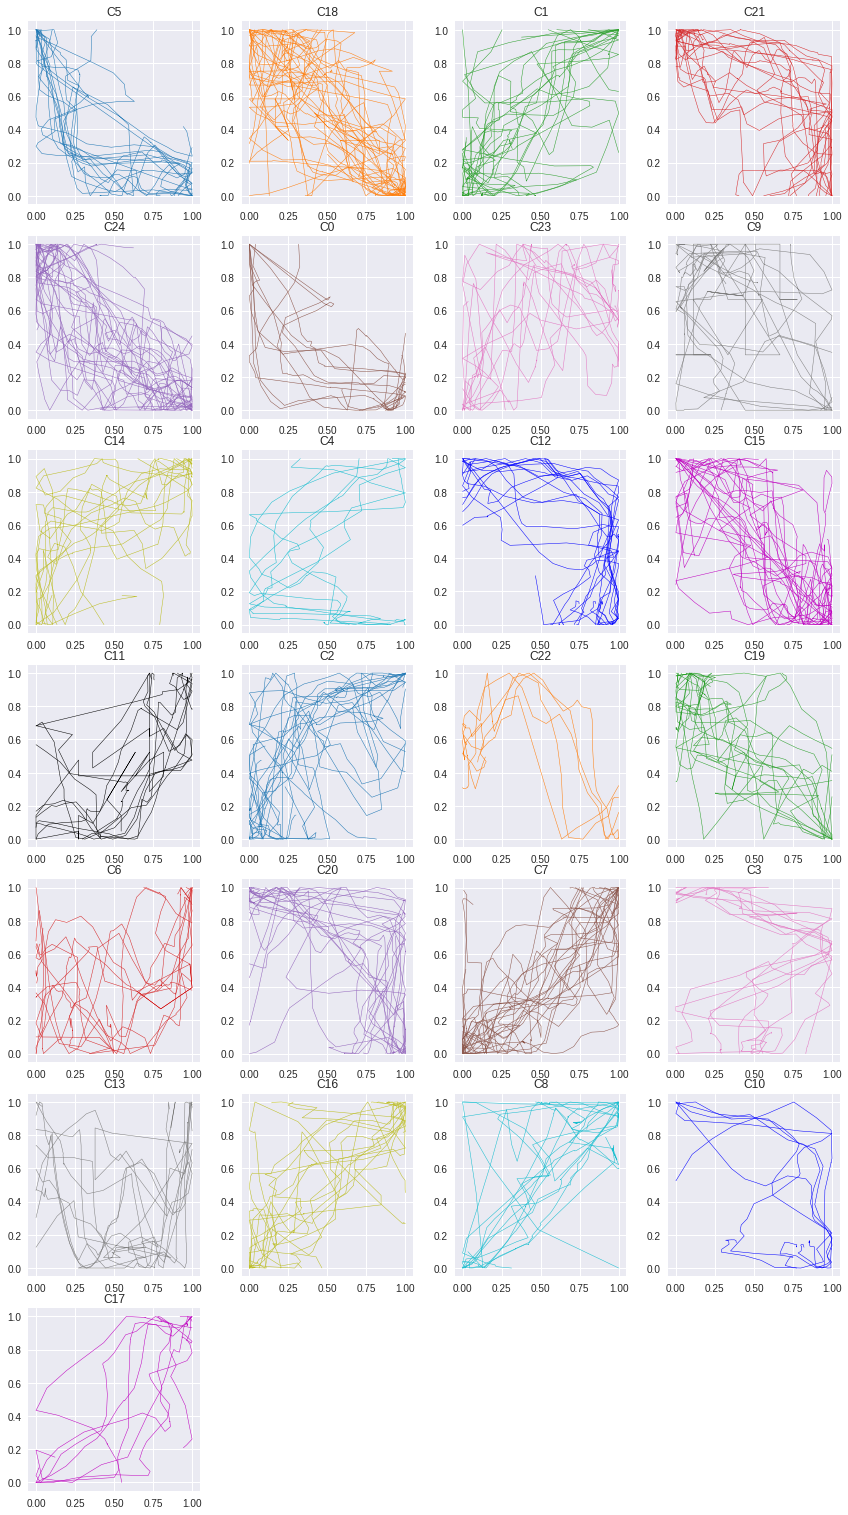
\includegraphics[width=\linewidth,height=\textheight,keepaspectratio]{figs/clusters/CLU_AP_ALL[MSM;c=1].png}
  \caption{Affinity Propagation: Move-Split-Merge, cost$=1$}
\end{figure}

\begin{figure}[h]
  \centering
  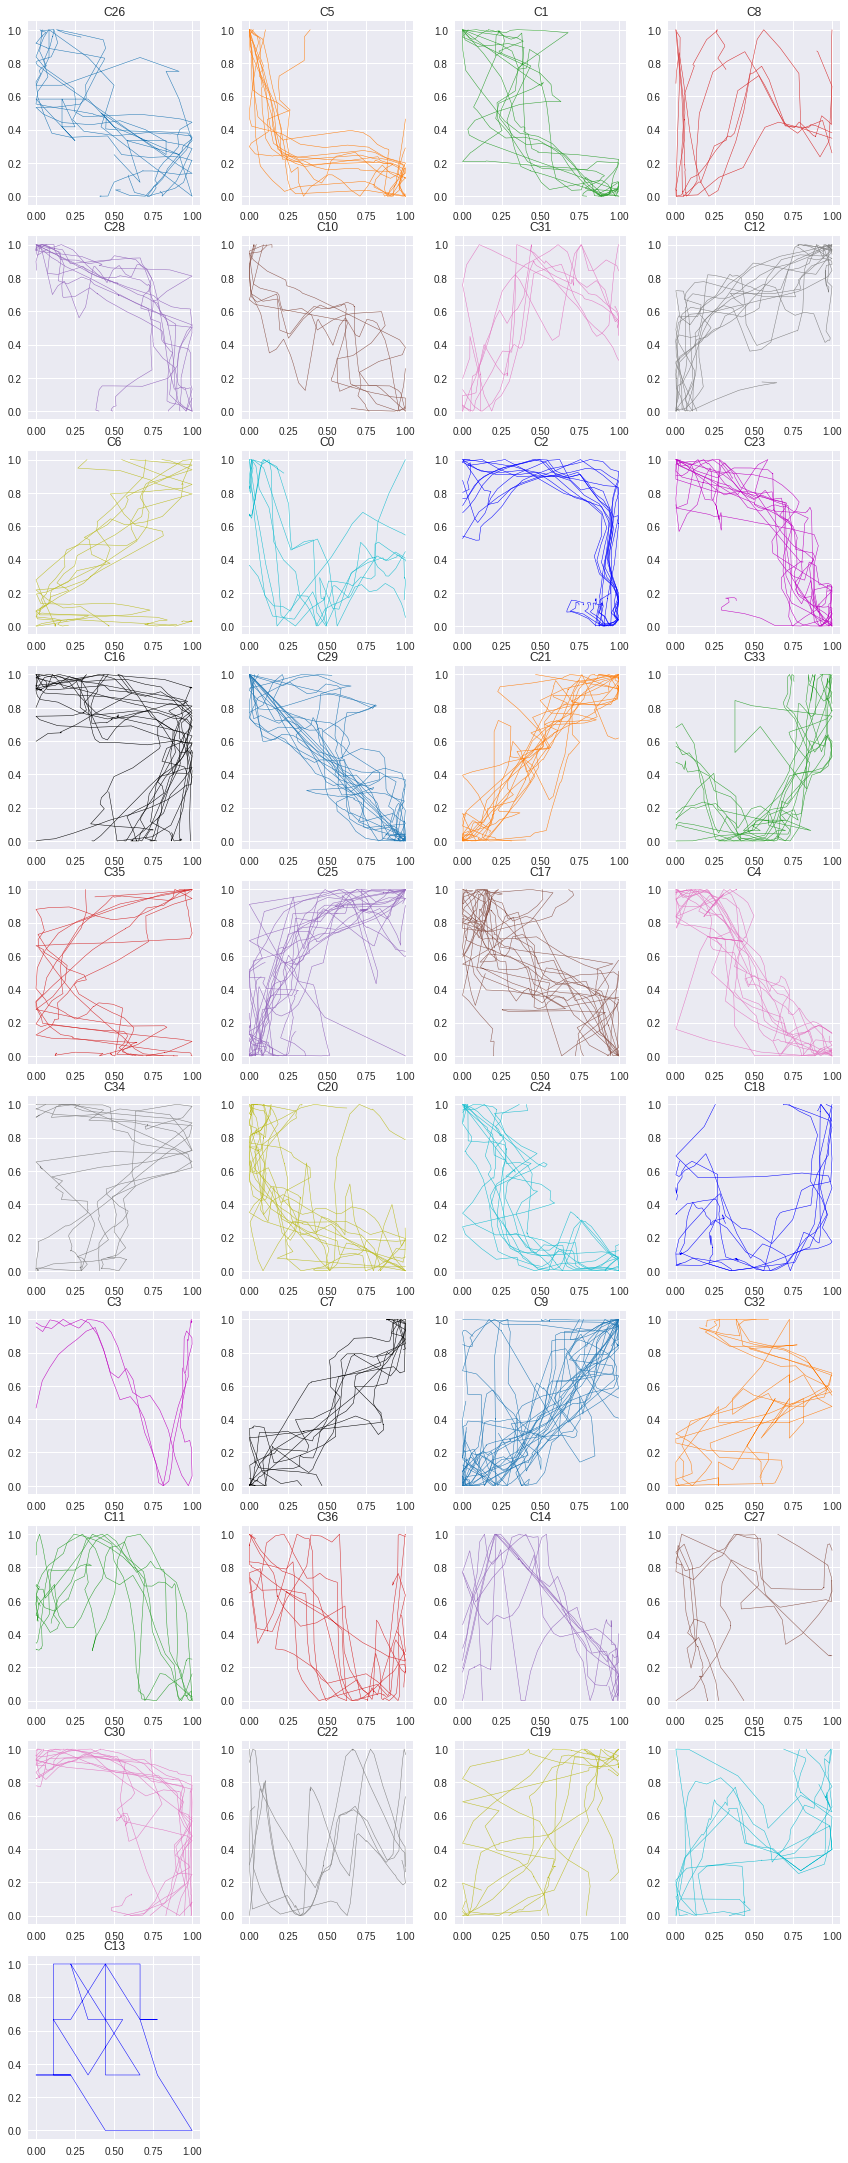
\includegraphics[width=\linewidth,height=\textheight,keepaspectratio]{figs/clusters/CLU_AP_ALL[MSM;c=.1].png}
  \caption{Affinity Propagation:Move-Split-Merge, cost$=0.1$}
\end{figure}

\begin{figure}[h]
  \centering
  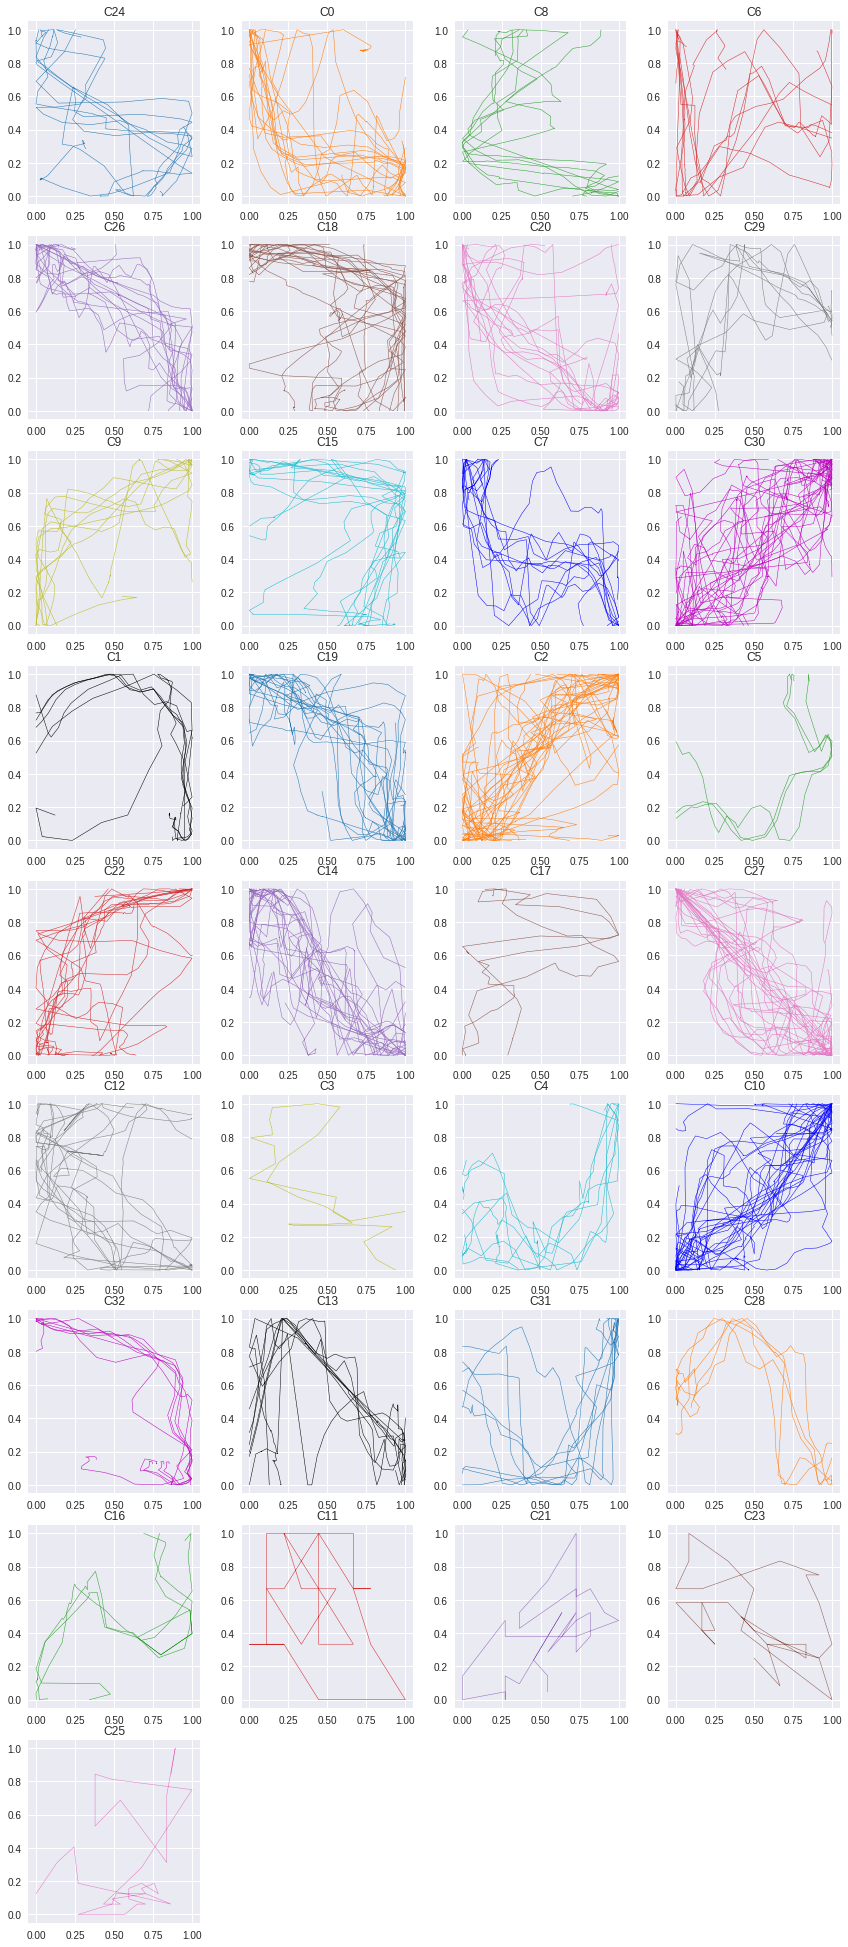
\includegraphics[width=\linewidth,height=\textheight,keepaspectratio]{figs/clusters/CLU_AP_ALL[MSM;c=.01].png}
  \caption{Affinity Propagation:Move-Split-Merge, cost$=0.01$}
\end{figure}

\begin{figure}[h]
  \centering
  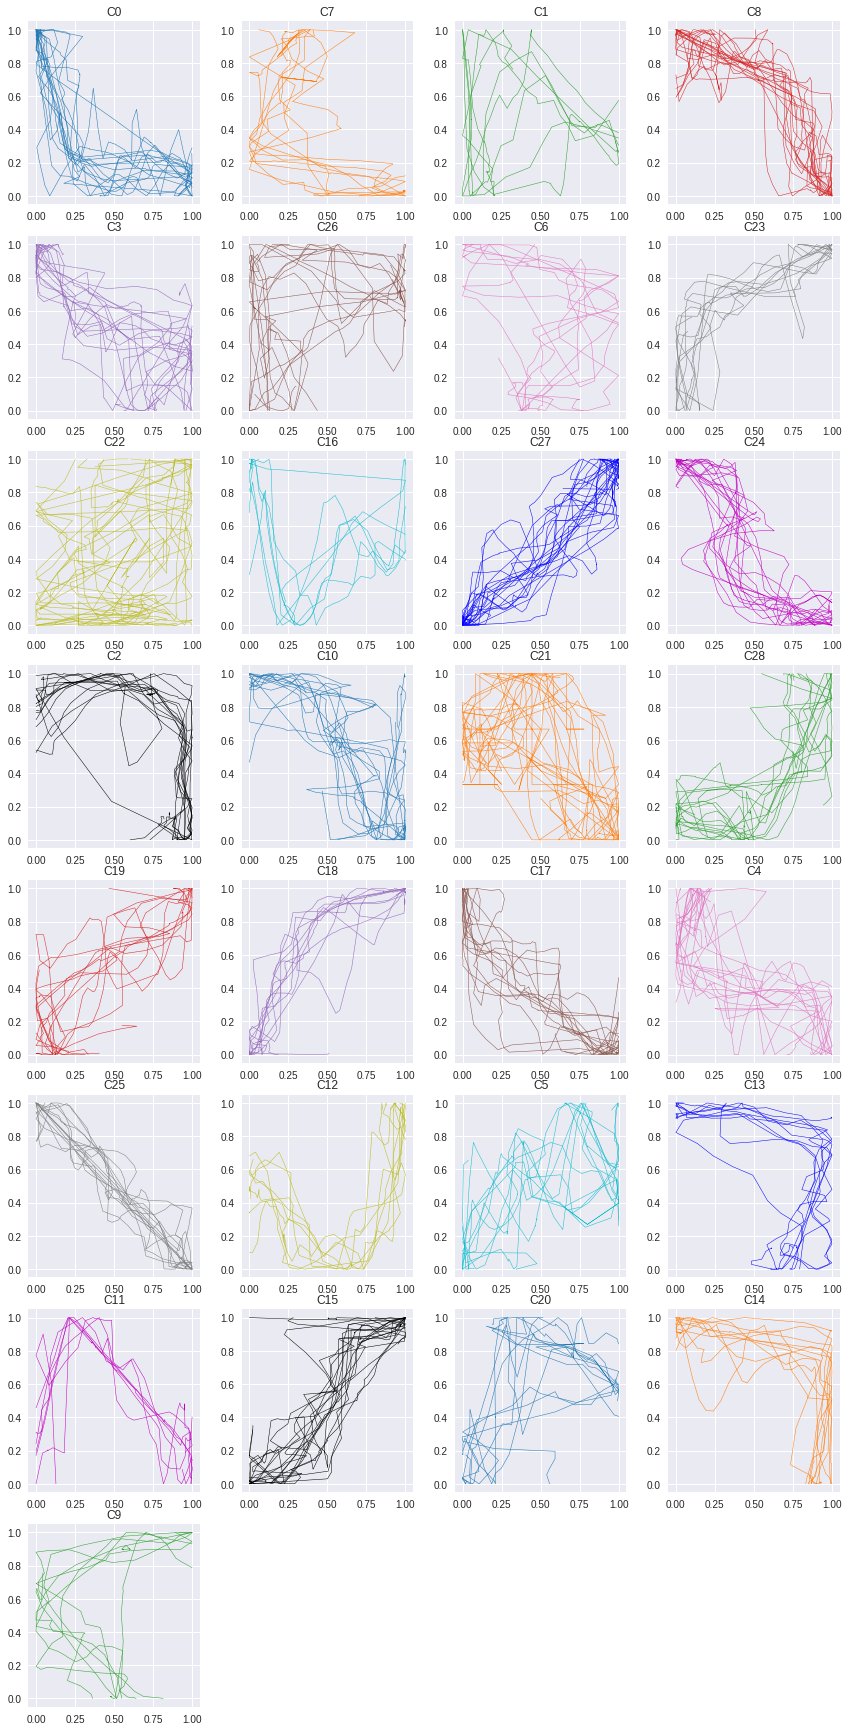
\includegraphics[width=\linewidth,height=\textheight,keepaspectratio]{figs/clusters/CLU_AP_ALL[SSPD].png}
  \caption{Affinity Propagation: Symmetrized Segment-Path Distance }
\end{figure}

\chapter{Agglomerative Hierarchical Clusters}
\label{app:h-clu}

\begin{figure}[h]
  \centering
  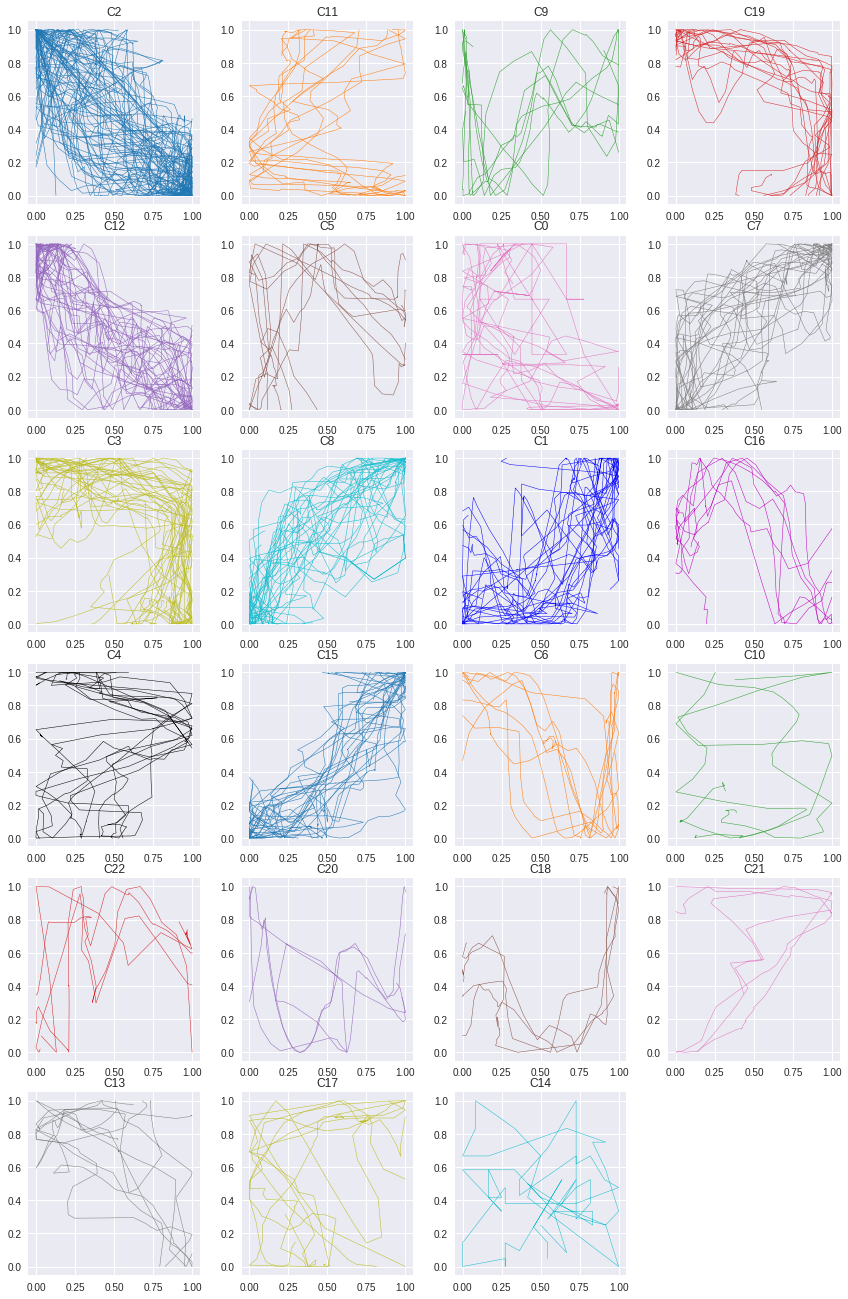
\includegraphics[width=\linewidth,height=\textheight,keepaspectratio]{figs/clusters/CLU_H_ALL[DTW].png}
  \caption{ Hierarchical Clusters: Dynamic Time Warping}
\end{figure}

\begin{figure}[h]
  \centering
  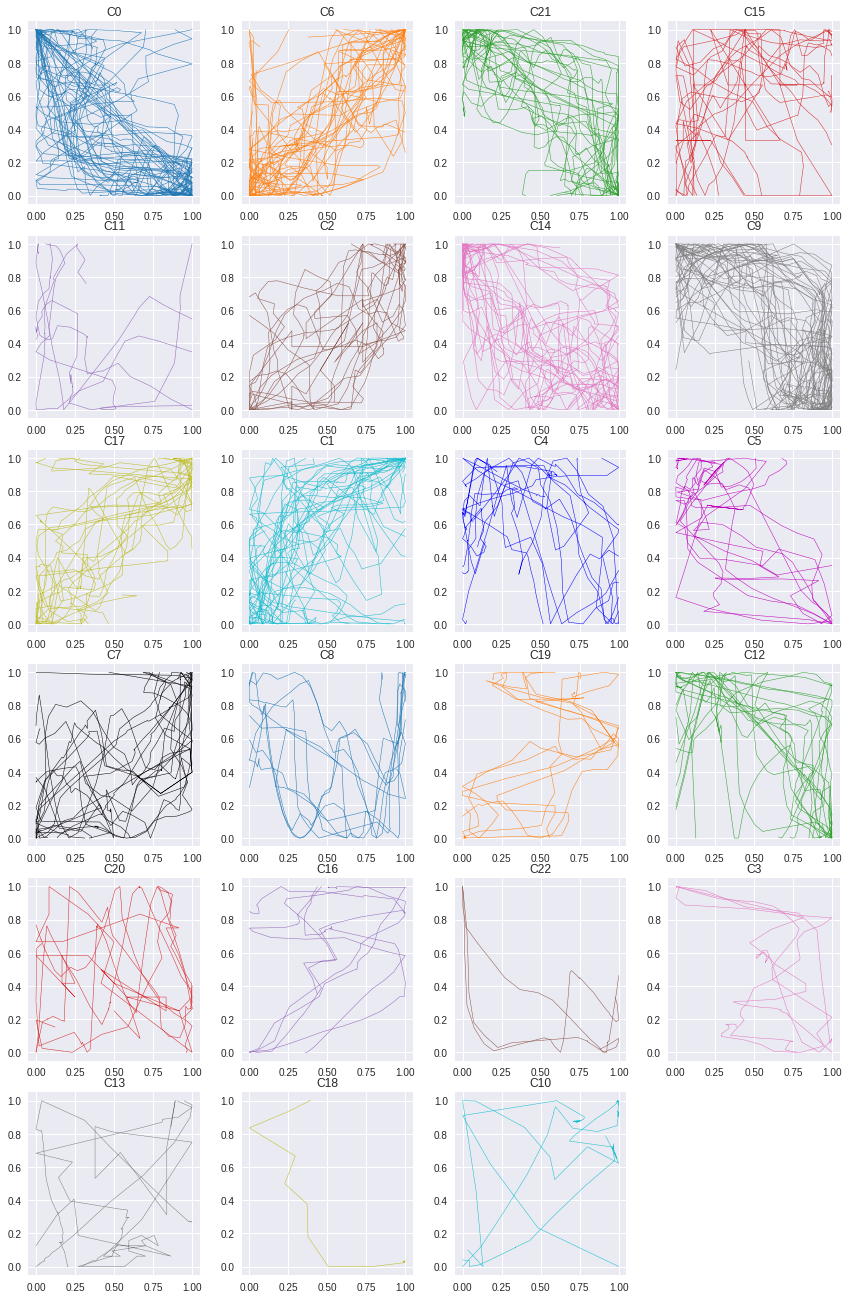
\includegraphics[width=\linewidth,height=\textheight,keepaspectratio]{figs/clusters/CLU_H_ALL[Ed].png}
  \caption{ Hierarchical Clusters: Euclidean Distance}
\end{figure}

\begin{figure}[h]
  \centering
  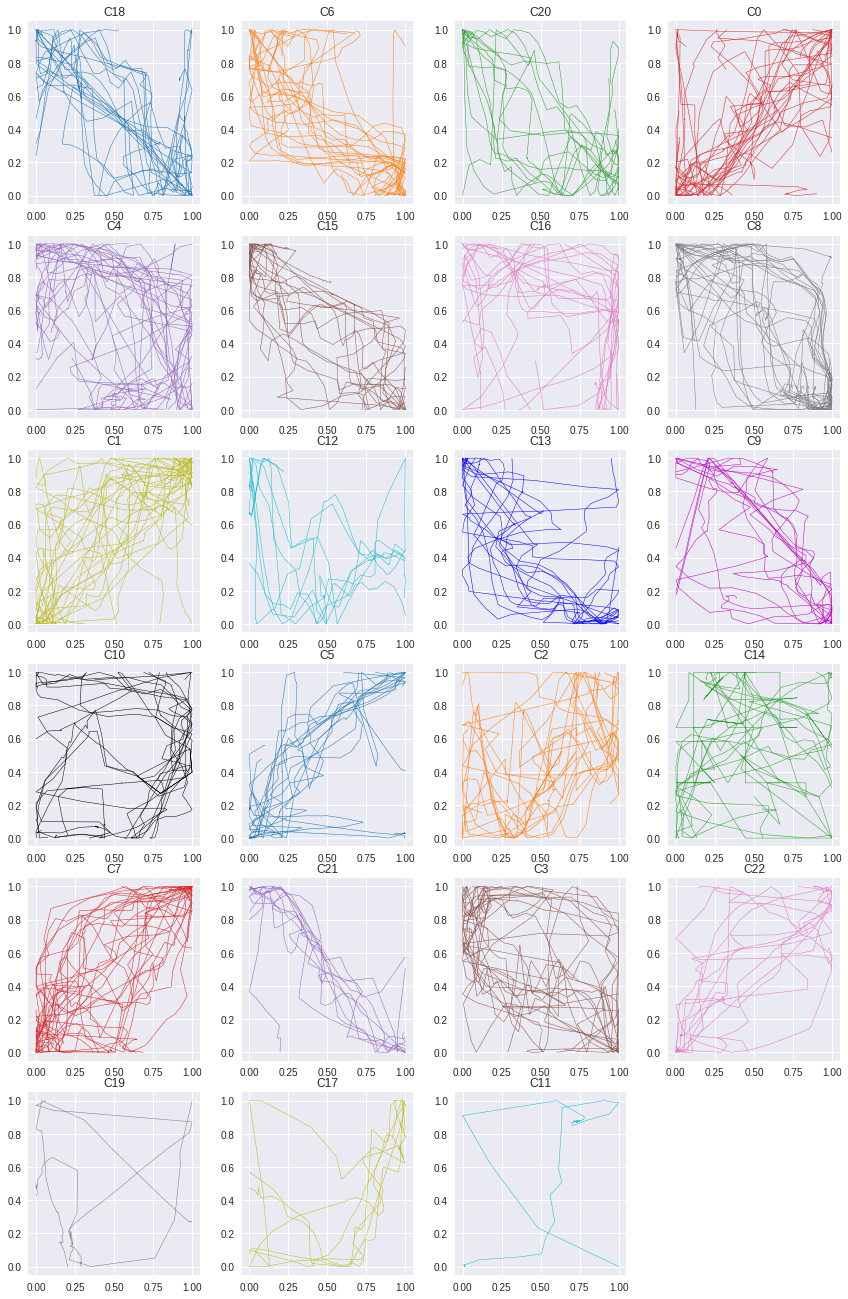
\includegraphics[width=\linewidth,height=\textheight,keepaspectratio]{figs/clusters/CLU_H_ALL[EDR;e=.101].png}
  \caption{ Hierarchical Clusters: Edit Distance on Real Sequence, $\epsilon=0.101$}
\end{figure}

\begin{figure}[h]
  \centering
  \includegraphics[width=\linewidth,height=\textheight,keepaspectratio]{figs/clusters/CLU_H_ALL[EDR;e=.203].png}
  \caption{ Hierarchical Clusters: Edit Distance on Real Sequence, $\epsilon=0.203$}
\end{figure}

\begin{figure}[h]
  \centering
  \includegraphics[width=\linewidth,height=\textheight,keepaspectratio]{figs/clusters/CLU_H_ALL[ERP;g=0,0].png}
  \caption{ Hierarchical Clusters: Edit Distance with Real Penalty}
\end{figure}

\begin{figure}[h]
  \centering
  \includegraphics[width=\linewidth,height=\textheight,keepaspectratio]{figs/clusters/CLU_H_ALL[Hd].png}
  \caption{ Hierarchical Clusters: Hausdorff Distance}
\end{figure}

\begin{figure}[h]
  \centering
  \includegraphics[width=\linewidth,height=\textheight,keepaspectratio]{figs/clusters/CLU_H_ALL[MSM;c=1].png}
  \caption{ Hierarchical Clusters: Move-Split-Merge, cost$=1$}
\end{figure}

\begin{figure}[h]
  \centering
  \includegraphics[width=\linewidth,height=\textheight,keepaspectratio]{figs/clusters/CLU_H_ALL[MSM;c=.1].png}
  \caption{ Hierarchical Clusters:Move-Split-Merge, cost$=0.1$}
\end{figure}

\begin{figure}[h]
  \centering
  \includegraphics[width=\linewidth,height=\textheight,keepaspectratio]{figs/clusters/CLU_H_ALL[MSM;c=.01].png}
  \caption{ Hierarchical Clusters:Move-Split-Merge, cost$=0.01$}
\end{figure}

\begin{figure}[h]
  \centering
  \includegraphics[width=\linewidth,height=\textheight,keepaspectratio]{figs/clusters/CLU_H_ALL[SSPD].png}
  \caption{ Hierarchical Clusters: Symmetrized Segment-Path Distance }
\end{figure}

\end{document}
